\chapter{Case Study thực tế (phần 2)}

\section{\textbf{Dự án 1: Tạo RAG system - hệ thống trả lời câu hỏi bằng tài liệu người dùng}}

\href{https://drive.google.com/file/d/1SwPcQe6HypodnICqbvVpzWVUKQA8_PLI/view?usp=sharing}{\textbf{\underline {Link tải workflow}}}

\begin{figure}[H]
    \centering
    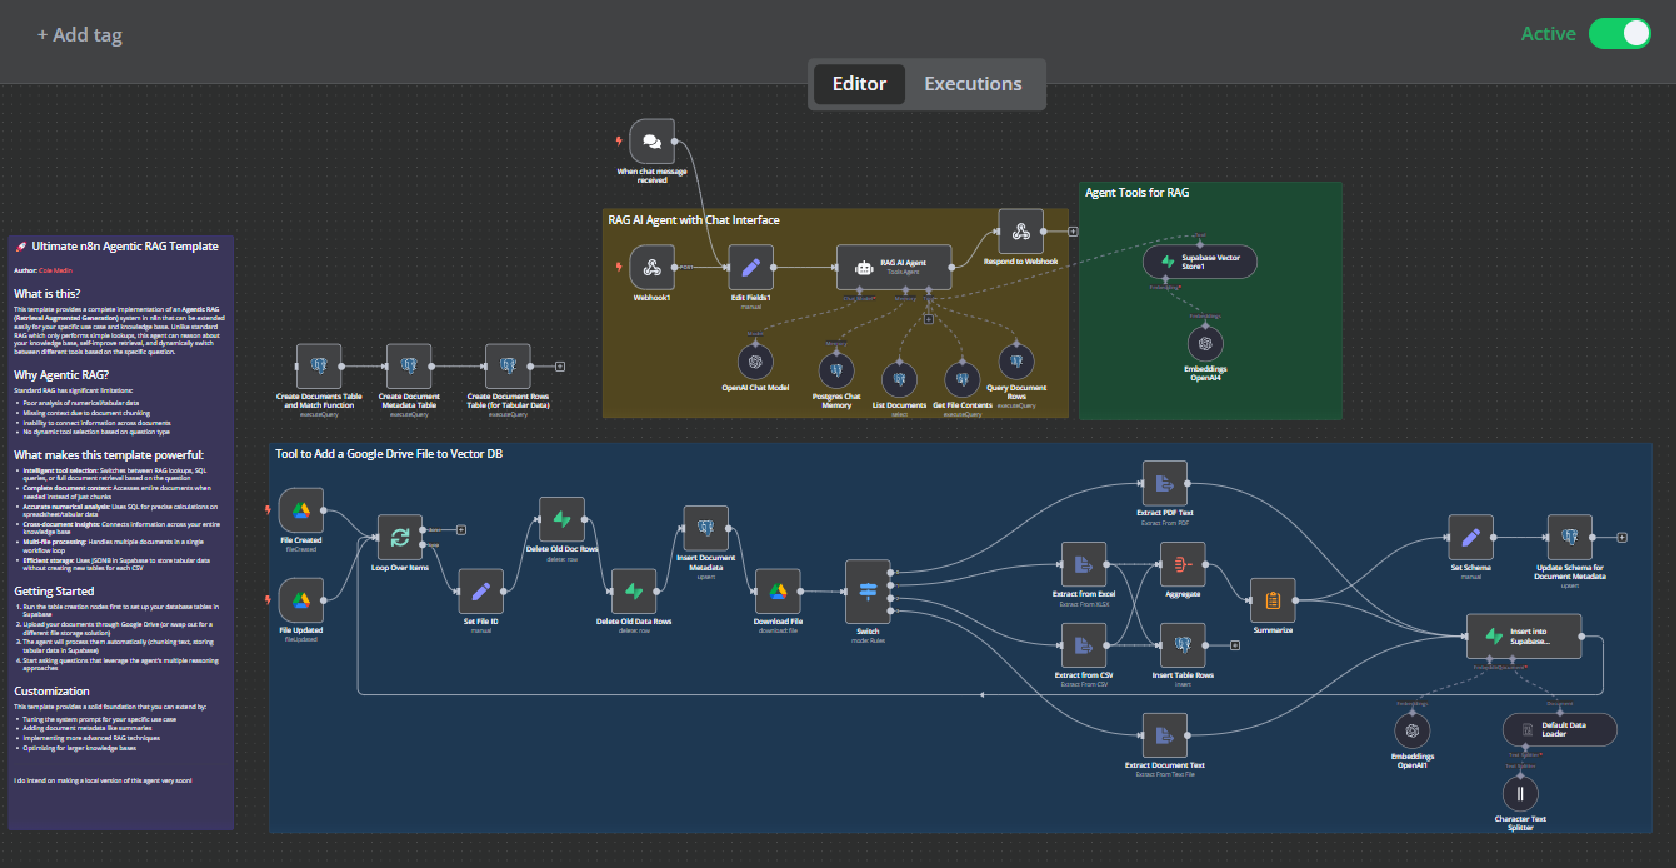
\includegraphics[width=1\textwidth]{images/1rag01.pdf}
    \caption{Workflow kết quả dự án 1}

\end{figure}

Workflow trong mã nguồn được chia sẻ là một hệ thống RAG (Retrieval Augmented Generation) nâng cao được xây dựng trên nền tảng n8n. Đây là một giải pháp toàn diện cho việc xử lý, lưu trữ và truy vấn thông tin từ nhiều loại tài liệu khác nhau.

\textbf{Chức năng chính:}
\begin{itemize}
    \item \textbf{Tự động xử lý tài liệu:} Phát hiện khi tài liệu mới được tạo hoặc cập nhật trong thư mục Google Drive; Hỗ trợ nhiều định dạng tài liệu: PDF, Google Docs, CSV, Excel, và văn bản thông thường; Tự động trích xuất nội dung từ các loại tài liệu khác nhau.
    
    \item \textbf{Xử lý thông minh dựa trên loại tài liệu:} Văn bản và PDF: Chia nhỏ thành các đoạn có nghĩa, tạo embedding và lưu vào Supabase; Dữ liệu bảng (CSV/Excel): Trích xuất cấu trúc và nội dung, lưu trữ thông tin metadata và dữ liệu hàng.
    
    \item \textbf{Lưu trữ dữ liệu hiệu quả:} Sử dụng bảng \texttt{documents} với vectơ embedding thông qua pgvector; Bảng \texttt{document\_metadata} lưu thông tin về tài liệu; Bảng \texttt{document\_rows} lưu dữ liệu từ các tệp CSV/Excel.
    
    \item \textbf{Giao diện trò chuyện AI thông minh:} API webhook để nhận yêu cầu từ người dùng; Agent AI có thể sử dụng nhiều công cụ khác nhau để trả lời câu hỏi; Hỗ trợ bộ nhớ trò chuyện qua PostgreSQL.
    
    \item \textbf{Khả năng truy vấn đa dạng:} Tìm kiếm tương tự ngữ nghĩa (RAG); Truy vấn SQL trực tiếp trên dữ liệu bảng; Truy xuất toàn bộ nội dung tài liệu khi cần thiết.
\end{itemize}

\textbf{Điểm nổi bật:}
\begin{itemize}
    \item \textbf{Kiến trúc RAG Agent thông minh:} Không chỉ đơn thuần là RAG thông thường, workflow này sử dụng cách tiếp cận "agent" cho phép LLM chọn công cụ phù hợp nhất để trả lời câu hỏi.
    
    \item \textbf{Xử lý tài liệu linh hoạt:} Tự động phát hiện định dạng tài liệu và áp dụng phương pháp xử lý phù hợp, không cần cấu hình riêng cho từng loại tài liệu.
    
    \item \textbf{Tối ưu cho dữ liệu số học:} Sử dụng SQL để thực hiện phân tích chính xác trên dữ liệu bảng, khắc phục hạn chế của RAG tiêu chuẩn với dữ liệu số học.
    
    \item \textbf{Khả năng mở rộng:} Thiết kế dễ dàng mở rộng để hỗ trợ thêm nguồn dữ liệu và công cụ mới.
    
    \item \textbf{Hiệu quả lưu trữ:} Sử dụng JSONB trong Supabase để lưu trữ dữ liệu bảng mà không cần tạo bảng mới cho mỗi tệp CSV.
    
    \item \textbf{Tận dụng công nghệ hiện đại:} Kết hợp pgvector, OpenAI Embeddings, và LLM để tạo hệ thống RAG hoàn chỉnh.
\end{itemize}

\textbf{Hướng dẫn thiết lập:}

\textit{Bước 1: Chuẩn bị cơ sở dữ liệu}
\begin{itemize}
    \item \textbf{Thiết lập Supabase:} Tạo tài khoản Supabase và dự án mới; Lưu thông tin kết nối: URL và API Key.
    \begin{figure}[H]
    \centering
    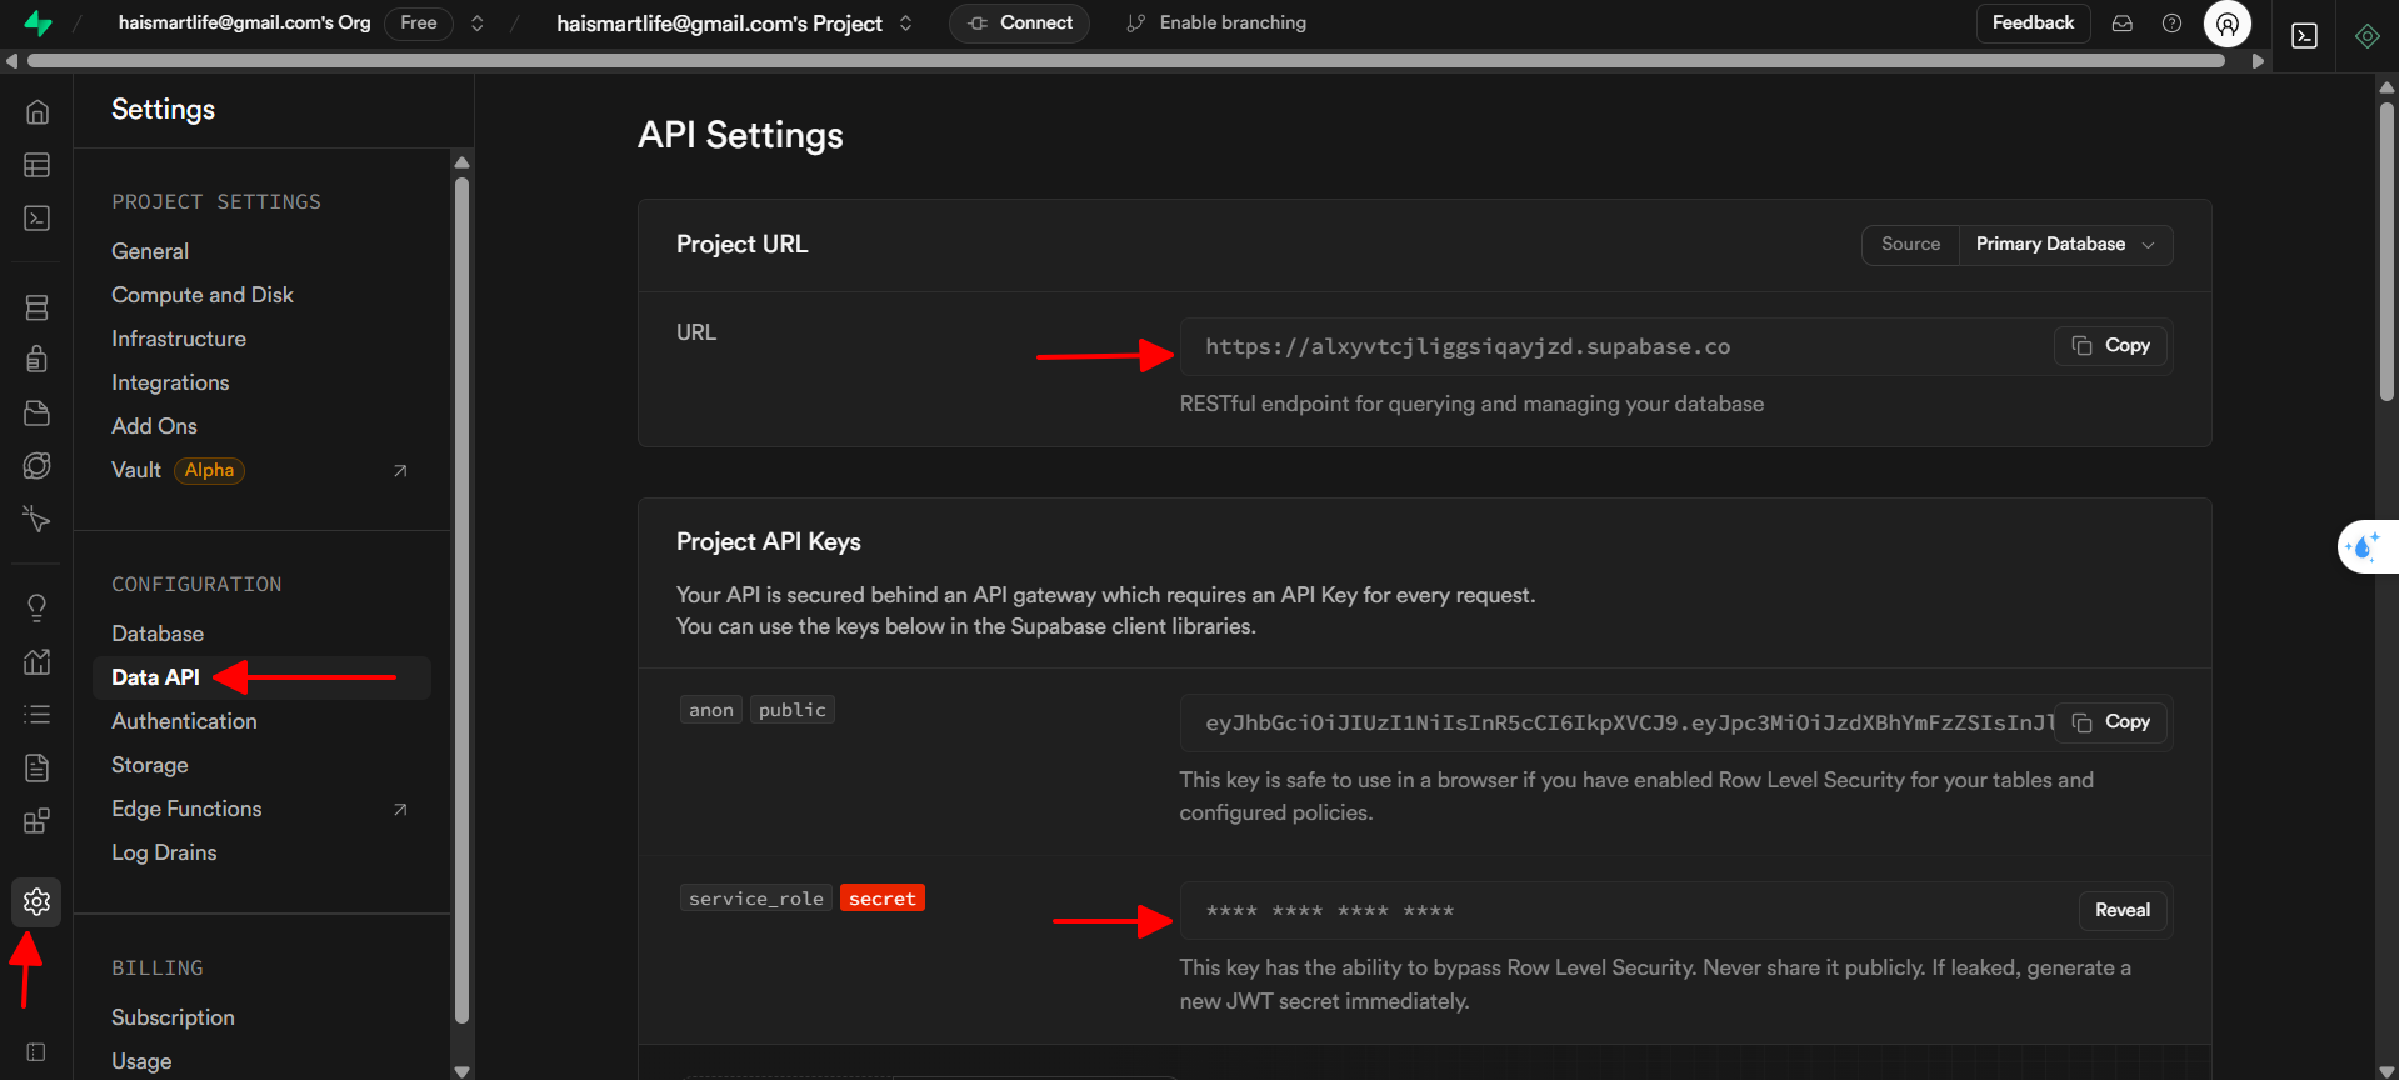
\includegraphics[width=1\textwidth]{images/1rag05.pdf}
    \caption{Thông tin Credential của Supabase}
    \end{figure}
    
    \item \textbf{Thiết lập PostgreSQL:} Đảm bảo PostgreSQL được cài đặt và hỗ trợ pgvector; Chạy các node tạo bảng theo thứ tự: \texttt{Create Documents Table and Match Function}, \texttt{Create Document Metadata Table}, \texttt{Create Document Rows Table}. Chạy 3 node này để tạo bảng và gọi thư viện tạo vector trong Supabase.\\
    \begin{figure}[H]
\centering
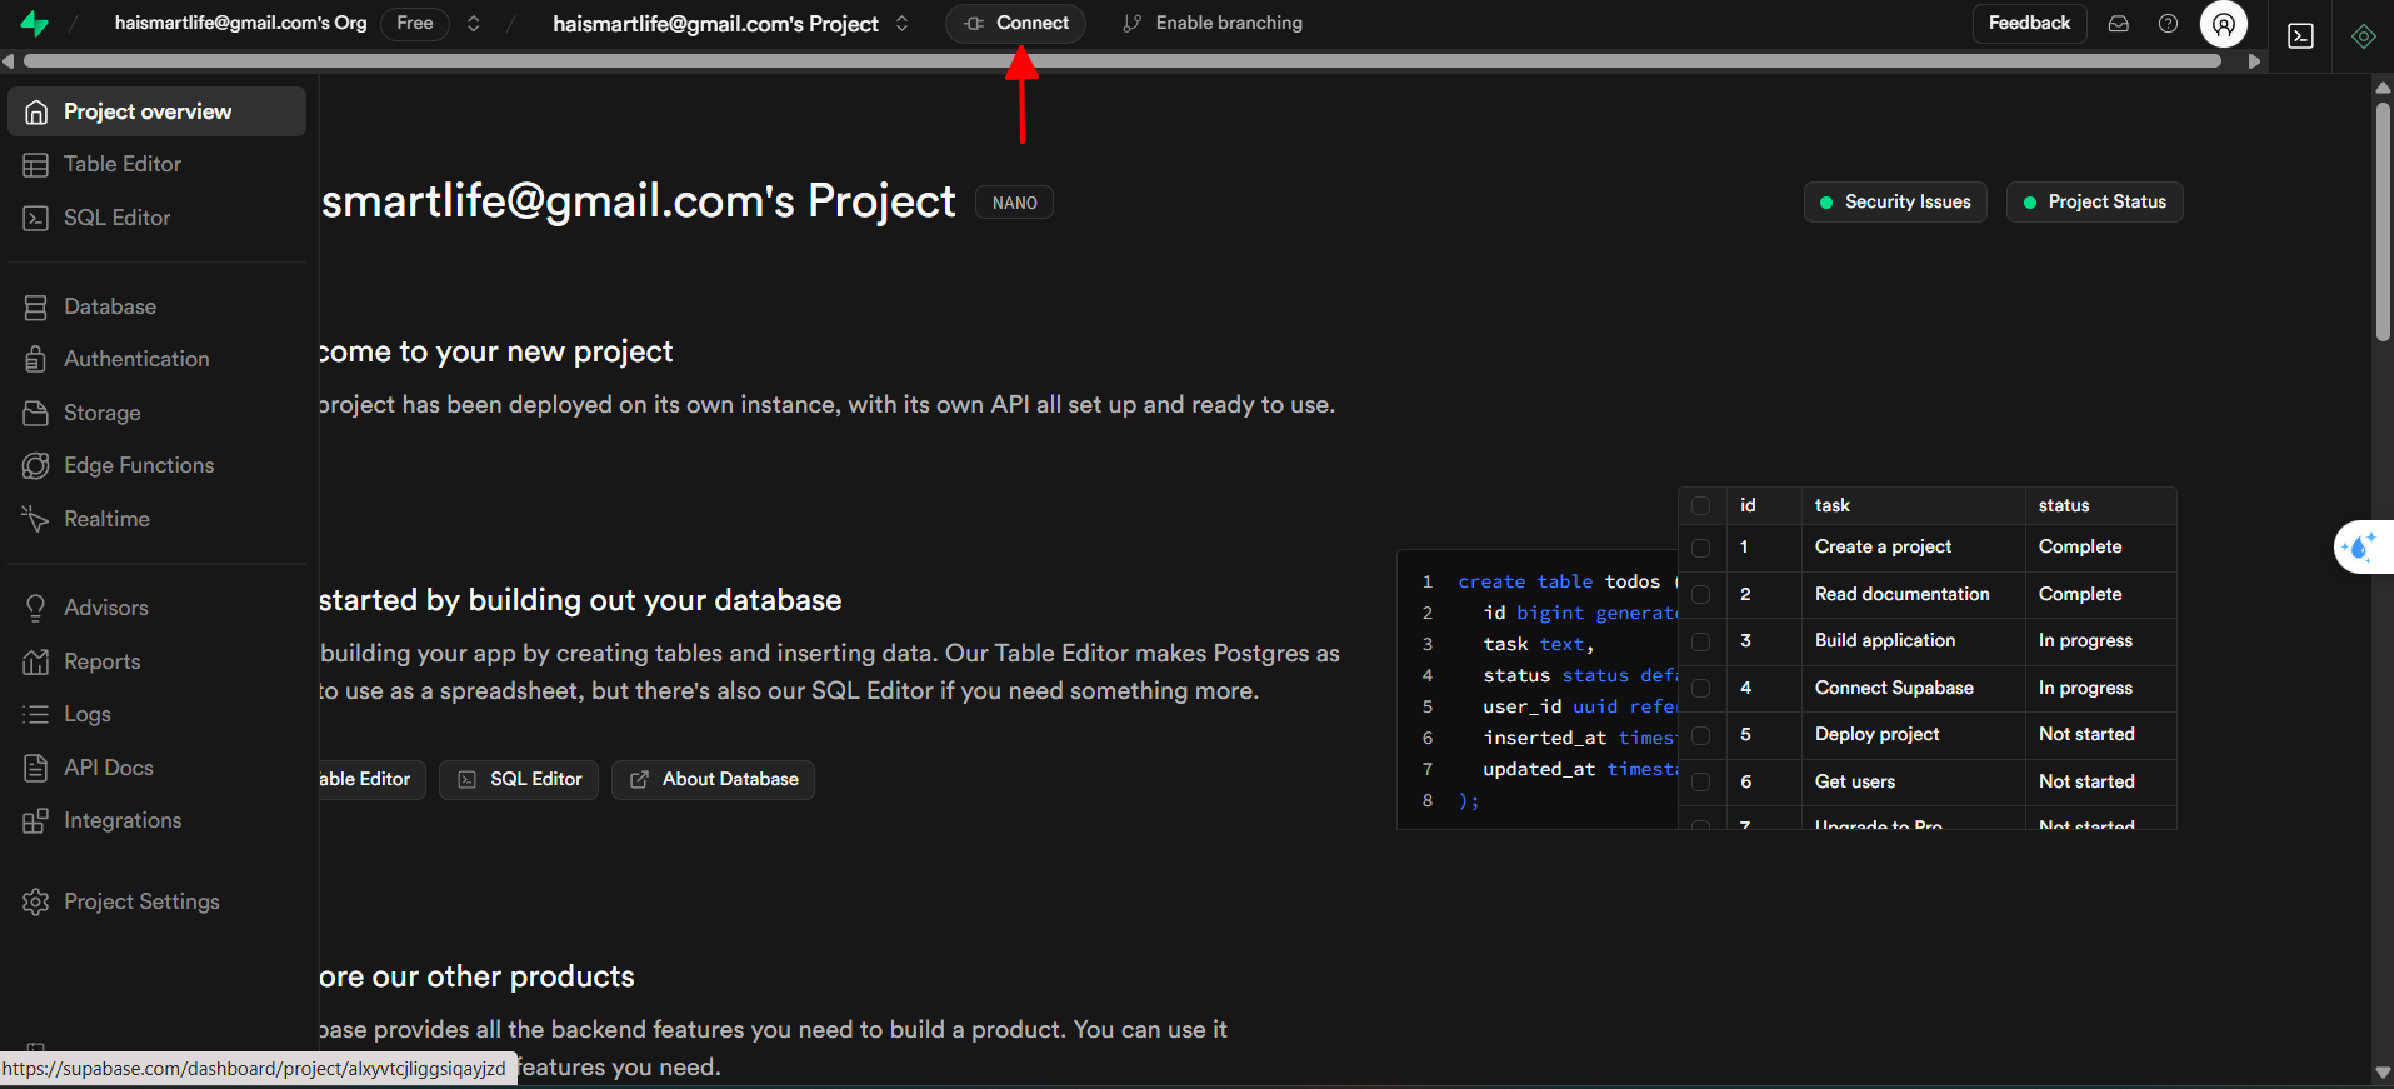
\includegraphics[width=1\textwidth]{images/1rag06.pdf}
\caption{Thông tin Credential của Postgres}
\end{figure}
Password của Postgres chính là mật khẩu lúc khởi tạo dự án. Nếu quên mật khẩu có thể vào cài đặt - Database - Database password và đặt lại. \\

Luu ý: phải chạy 3 node postgres trước khi upload file lên googledrive, để tạo bảng và khởi tạo biến vector trước. Nếu không sẽ bị lỗi và không chạy được\\

\end{itemize}
    

    
\begin{figure}[H]
\centering
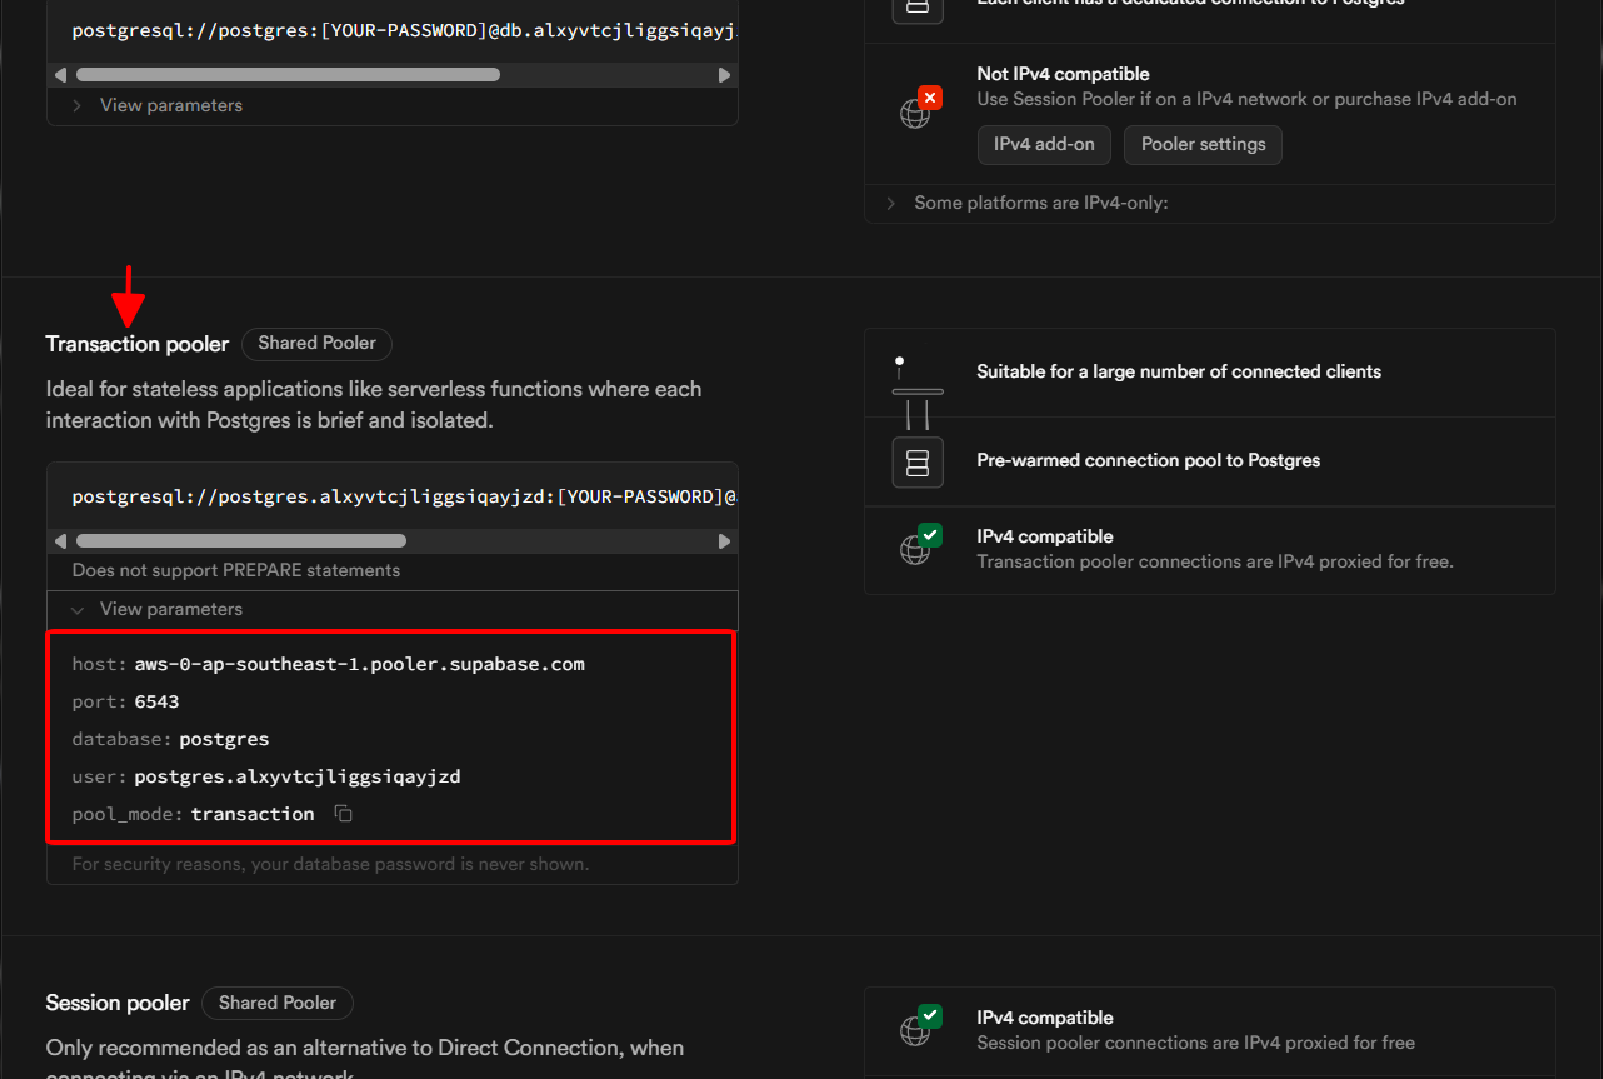
\includegraphics[width=1\textwidth]{images/1rag07.pdf}
\caption{Thông tin Credential của Postgres}
\end{figure}
    
    

\textit{Bước 2: Cấu hình Google Drive}
\begin{itemize}
    \item \textbf{Thiết lập OAuth:} Tạo OAuth credentials trong Google Developer Console; Thêm thông tin xác thực vào n8n.
    
    \item \textbf{Cấu hình thư mục:} Tạo thư mục riêng để chứa tài liệu cho bot; Lấy ID thư mục và cấu hình trong các node \texttt{File Created} và \texttt{File Updated}.
\end{itemize}

\textit{Bước 3: Cấu hình OpenAI API}
\begin{itemize}
    \item \textbf{Tạo API key:} Đăng ký tài khoản và tạo API key từ OpenAI; Thêm thông tin xác thực vào n8n.
    
    \item \textbf{Cấu hình model:} Cấu hình mô hình embeddings (text-embedding-3-small); Cấu hình mô hình chat (gpt-4 hoặc tương tự).
\end{itemize}

\textit{Bước 4: Thiết lập Workflow}
\begin{itemize}
    \item \textbf{Xử lý tài liệu:} Cấu hình node trigger với ID thư mục Google Drive; Thiết lập các node xử lý tài liệu; Cấu hình node \texttt{Switch} để định tuyến luồng dữ liệu.
    
    \item \textbf{Vector embedding:} Cấu hình \texttt{Character Text Splitter} (chunk 1000 ký tự, overlap 100 ký tự); Cấu hình \texttt{Embeddings OpenAI1}; Thiết lập \texttt{Insert into Supabase Vectorstore}.
    
    \item \textbf{Xử lý dữ liệu bảng:} Cấu hình \texttt{Insert Table Rows}; Thiết lập \texttt{Update Schema for Document Metadata}.
    
    \item \textbf{AI Agent:} Cấu hình webhook; Thiết lập \texttt{RAG AI Agent} với system prompt; Cấu hình các công cụ; Thiết lập \texttt{Postgres Chat Memory}.
\end{itemize}

\textit{Bước 5: Tích hợp giao diện người dùng}
\begin{itemize}
    \item \textbf{Thiết lập webhook:} Lấy URL webhook từ node \texttt{Webhook1}; Cấu hình API endpoint trong ứng dụng frontend - Lovable.dev để tạo giao diện frontend.
    
    \begin{figure}[H]
    \centering
    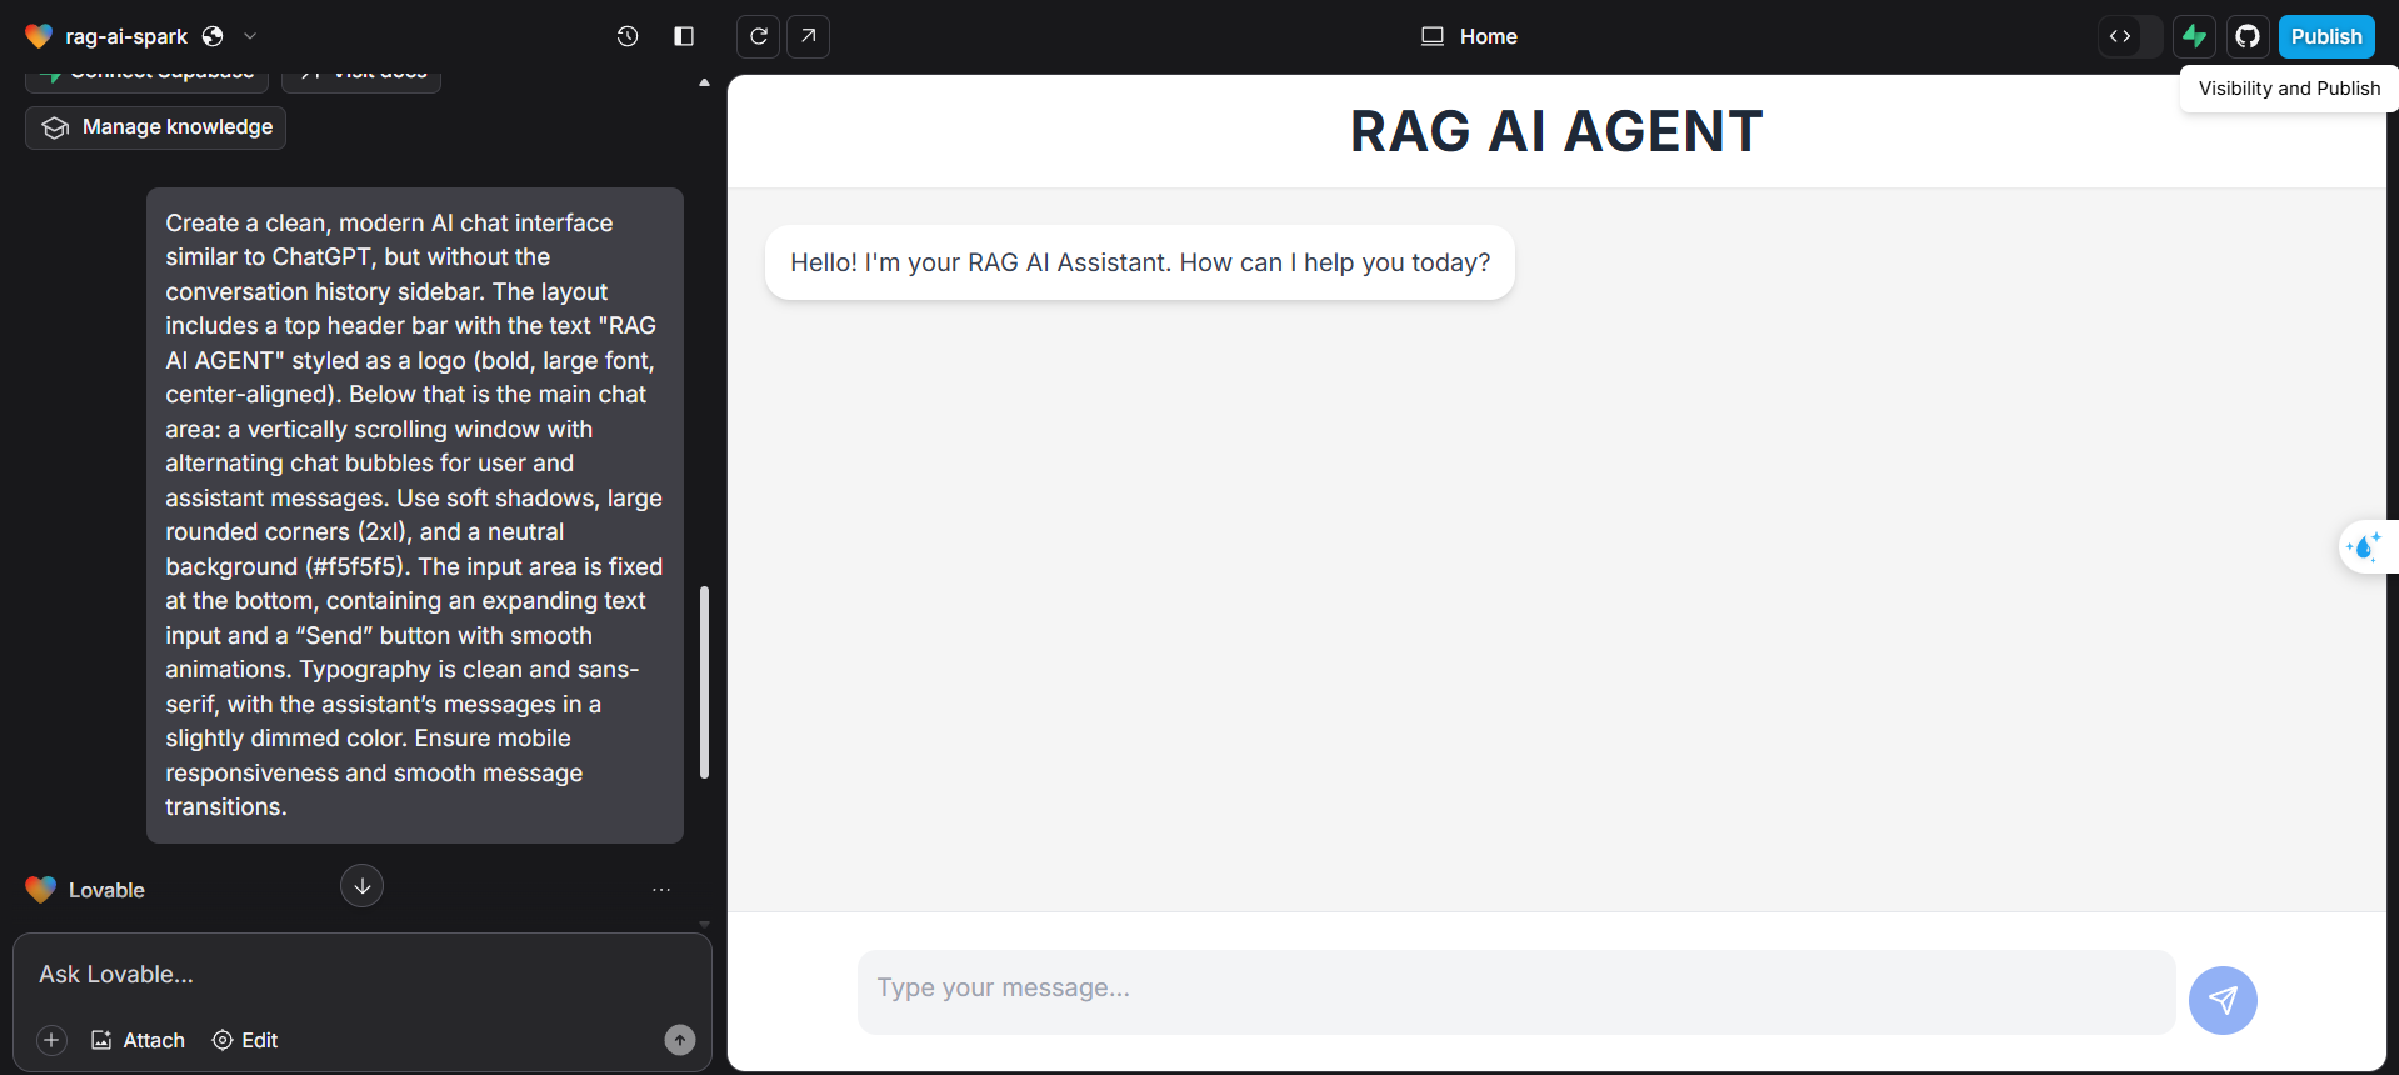
\includegraphics[width=1\textwidth]{images/1rag02.pdf}
    \caption{Workflow giao diện web tương tác}
    \end{figure}
Đây là một kỹ thuật khá hay để tạo giao diện thân thiện với người dùng và cũng rất đơn giản để làm được.\\

\textbf{Step 1:} Truy cập web \url{https://lovable.dev/} - Đăng nhập và paste Prompt sau vào ô thoại của Lovable, trang web sẽ tự tạo frontend cho bạn (có thẻ tự thay đổi đổi có giao diện phù hợp mỗi người.

\textbf{Prompt:} \emph{Create a clean, modern AI chat interface similar to ChatGPT, but without the conversation history sidebar. The layout includes a top header bar with the text \textquotedblleft RAG AI AGENT \textquotedblright{} styled as a logo (bold, large font, center-aligned). Below that is the main chat area: a vertically scrolling window with alternating chat bubbles for user and assistant messages. Use soft shadows, large rounded corners (2xl), and a neutral background (\#f5f5f5). The input area is fixed at the bottom, containing an expanding text input and a \textquotedblleft Send\textquotedblright{} button with smooth animations. Typography is clean and sans-serif, with the assistant’s messages in a slightly dimmed color. Ensure mobile responsiveness and smooth message transitions.}\\

\textbf{Step 2:} Sau khi giao diện ban đầu được tạo thì tiếp tục nhập prompt chứa webhook n8n của bạn vào. Lưu ý URL này là của Production URL. \\

\textbf{Prompt:} \emph{
Khi tôi nhấn nút gửi thì dữ liệu đến webhook as a post request: nhập URL webhook của bạn}

$\Rightarrow$ Sau khi đã tạo xong giao diện web chúng ta cần publish nó lên như hình bên dưới. Như vậy các bạn đã tạo được một giao diện frontend kết nối với backend là n8n để thực hiện lệnh.
\end{itemize}    
    \begin{figure}[H]
    \centering
    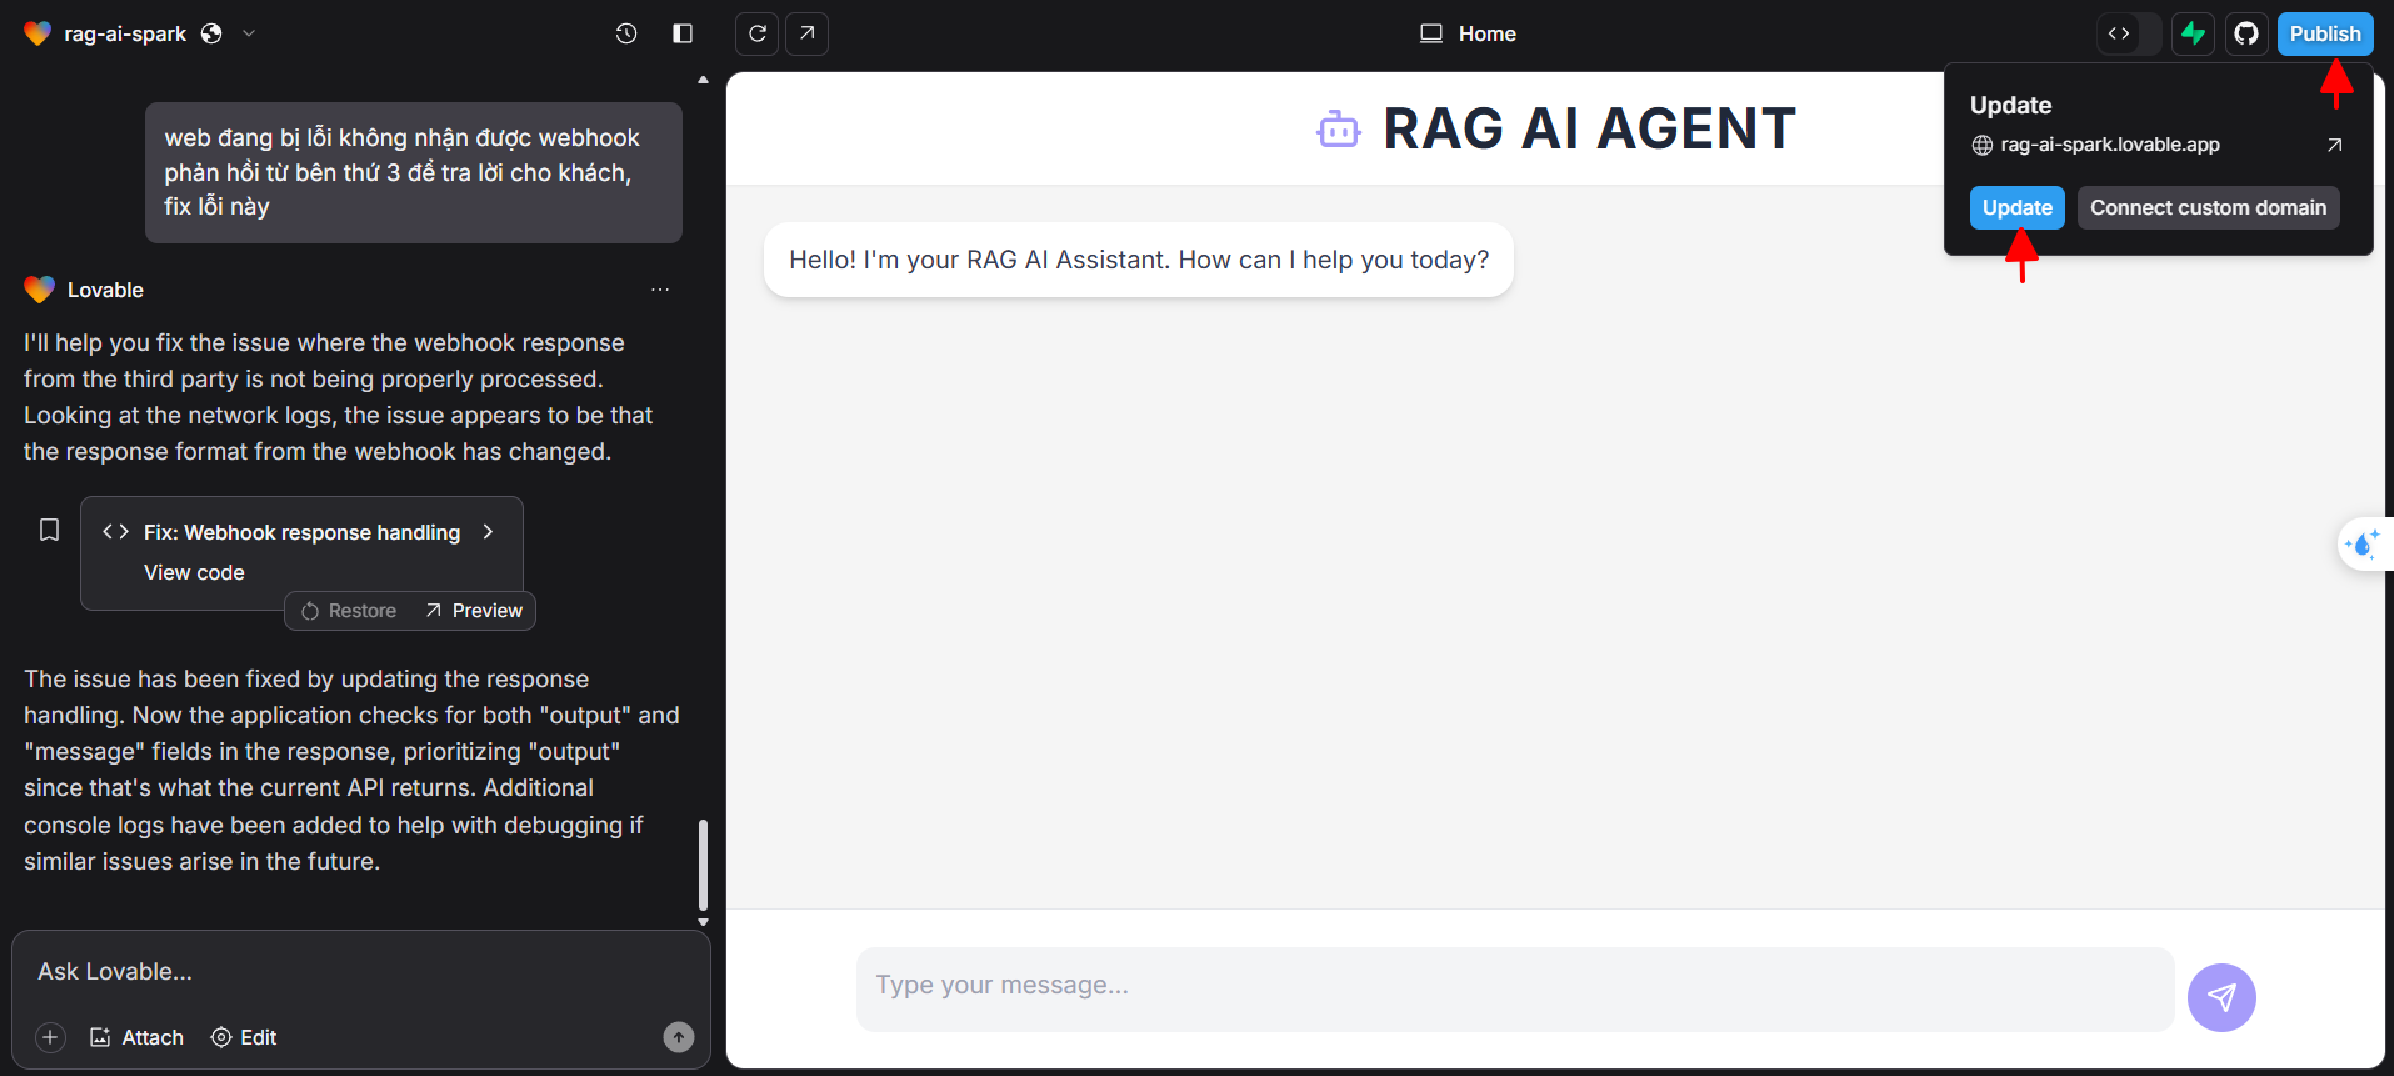
\includegraphics[width=1\textwidth]{images/1rag03.pdf}
    \caption{Publish web để có thể truy cập bằng subdomain}
    \end{figure}
    


\textit{Bước 6: Kiểm thử và tối ưu}
\begin{itemize}
    \item \textbf{Thử nghiệm tài liệu:} Tải lên các loại tài liệu khác nhau; Xác nhận xử lý và lưu trữ chính xác.
    
    \item \textbf{Kiểm tra truy vấn:} Thử nghiệm với các loại câu hỏi; Đánh giá hiệu quả RAG và SQL; Tinh chỉnh system prompt.
    
    \item \textbf{Tối ưu:} Điều chỉnh kích thước chunk và overlap; Tối ưu truy vấn vector; Cải tiến system prompt.
\end{itemize}



Workflow này là một bản mẫu mạnh mẽ cho hệ thống RAG Agent và có thể được tùy chỉnh để phù hợp với nhiều trường hợp sử dụng khác nhau, từ hệ thống hỗ trợ khách hàng đến phân tích dữ liệu nội bộ.\\



\newpage
%-------------------------------------------------------------------------

%-----------------------------------------------------------------------------
\clearpage

\section{\textbf{Dự án 2: Tự tạo tính năng gửi thông báo đến người đăng ký cho Blog cá nhân}}


\begin{figure}[htbp]
    \centering
    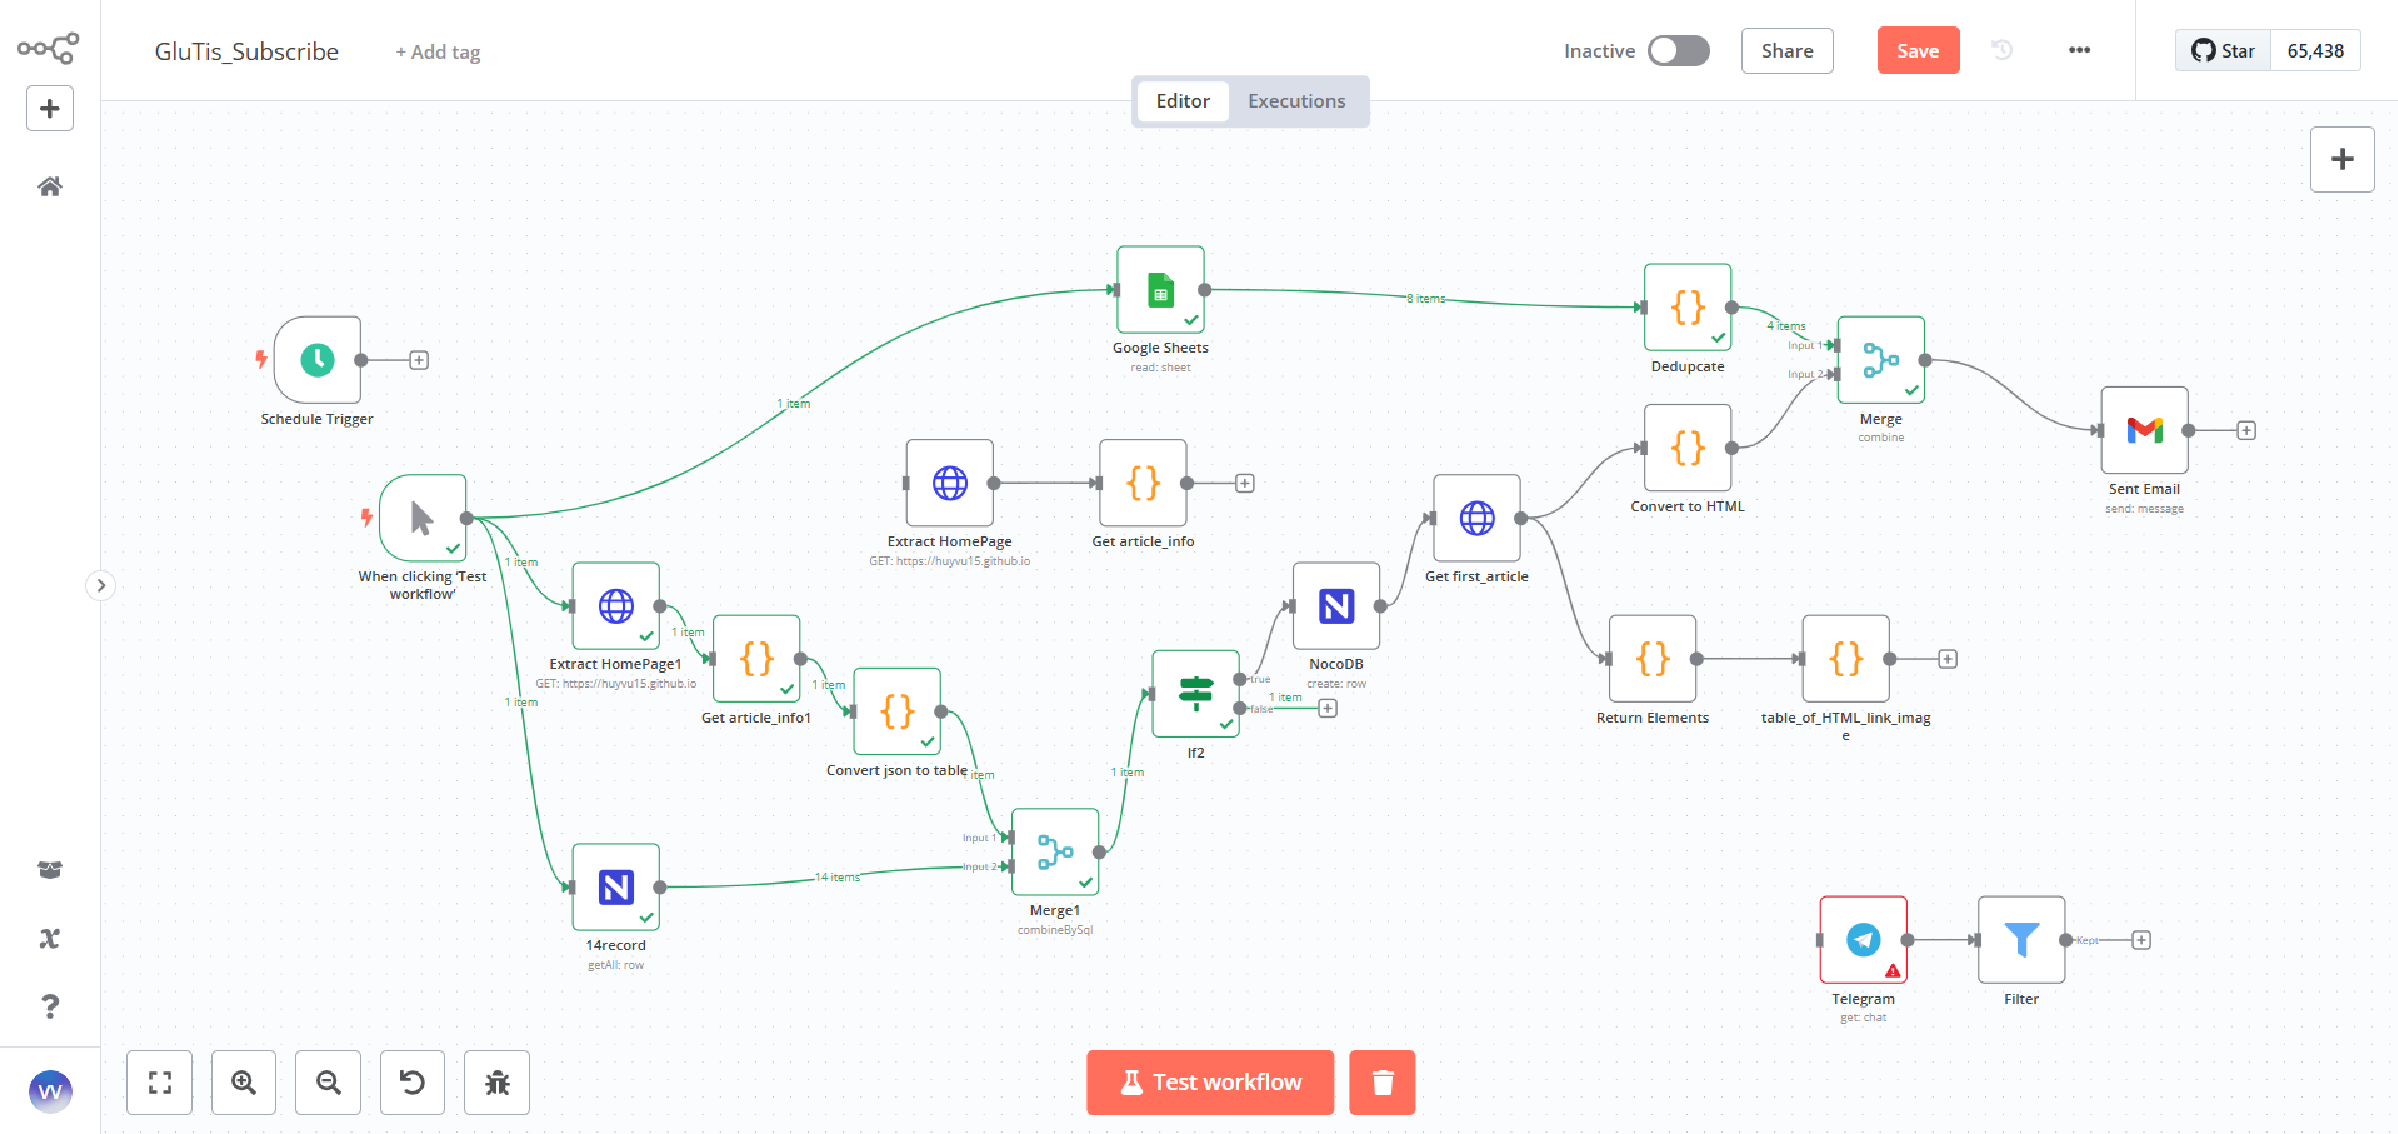
\includegraphics[width=1\linewidth]{Chap1-7/glutis-subscribe.pdf}
    \caption{Workflow subscribe}
\end{figure}


\subsection{Câu chuyện}
Mình có một trang Blog cá nhân là \href{https://glutis.is-a.dev/}{glutis.is-a.dev/}. Trang blog này hoàn toàn dựa trên một framework sẵn có. Một ngày mình nghĩ rằng người đọc cần nhận thông báo mỗi khi trang ra blog mới. 

$\Rightarrow$ Mình đã nghĩ tới việc tạo ra tính năng này cho chính blog cá nhân bằng n8n


\subsection{Tạo trang đăng ký}

\begin{figure}[htbp]
    \centering
    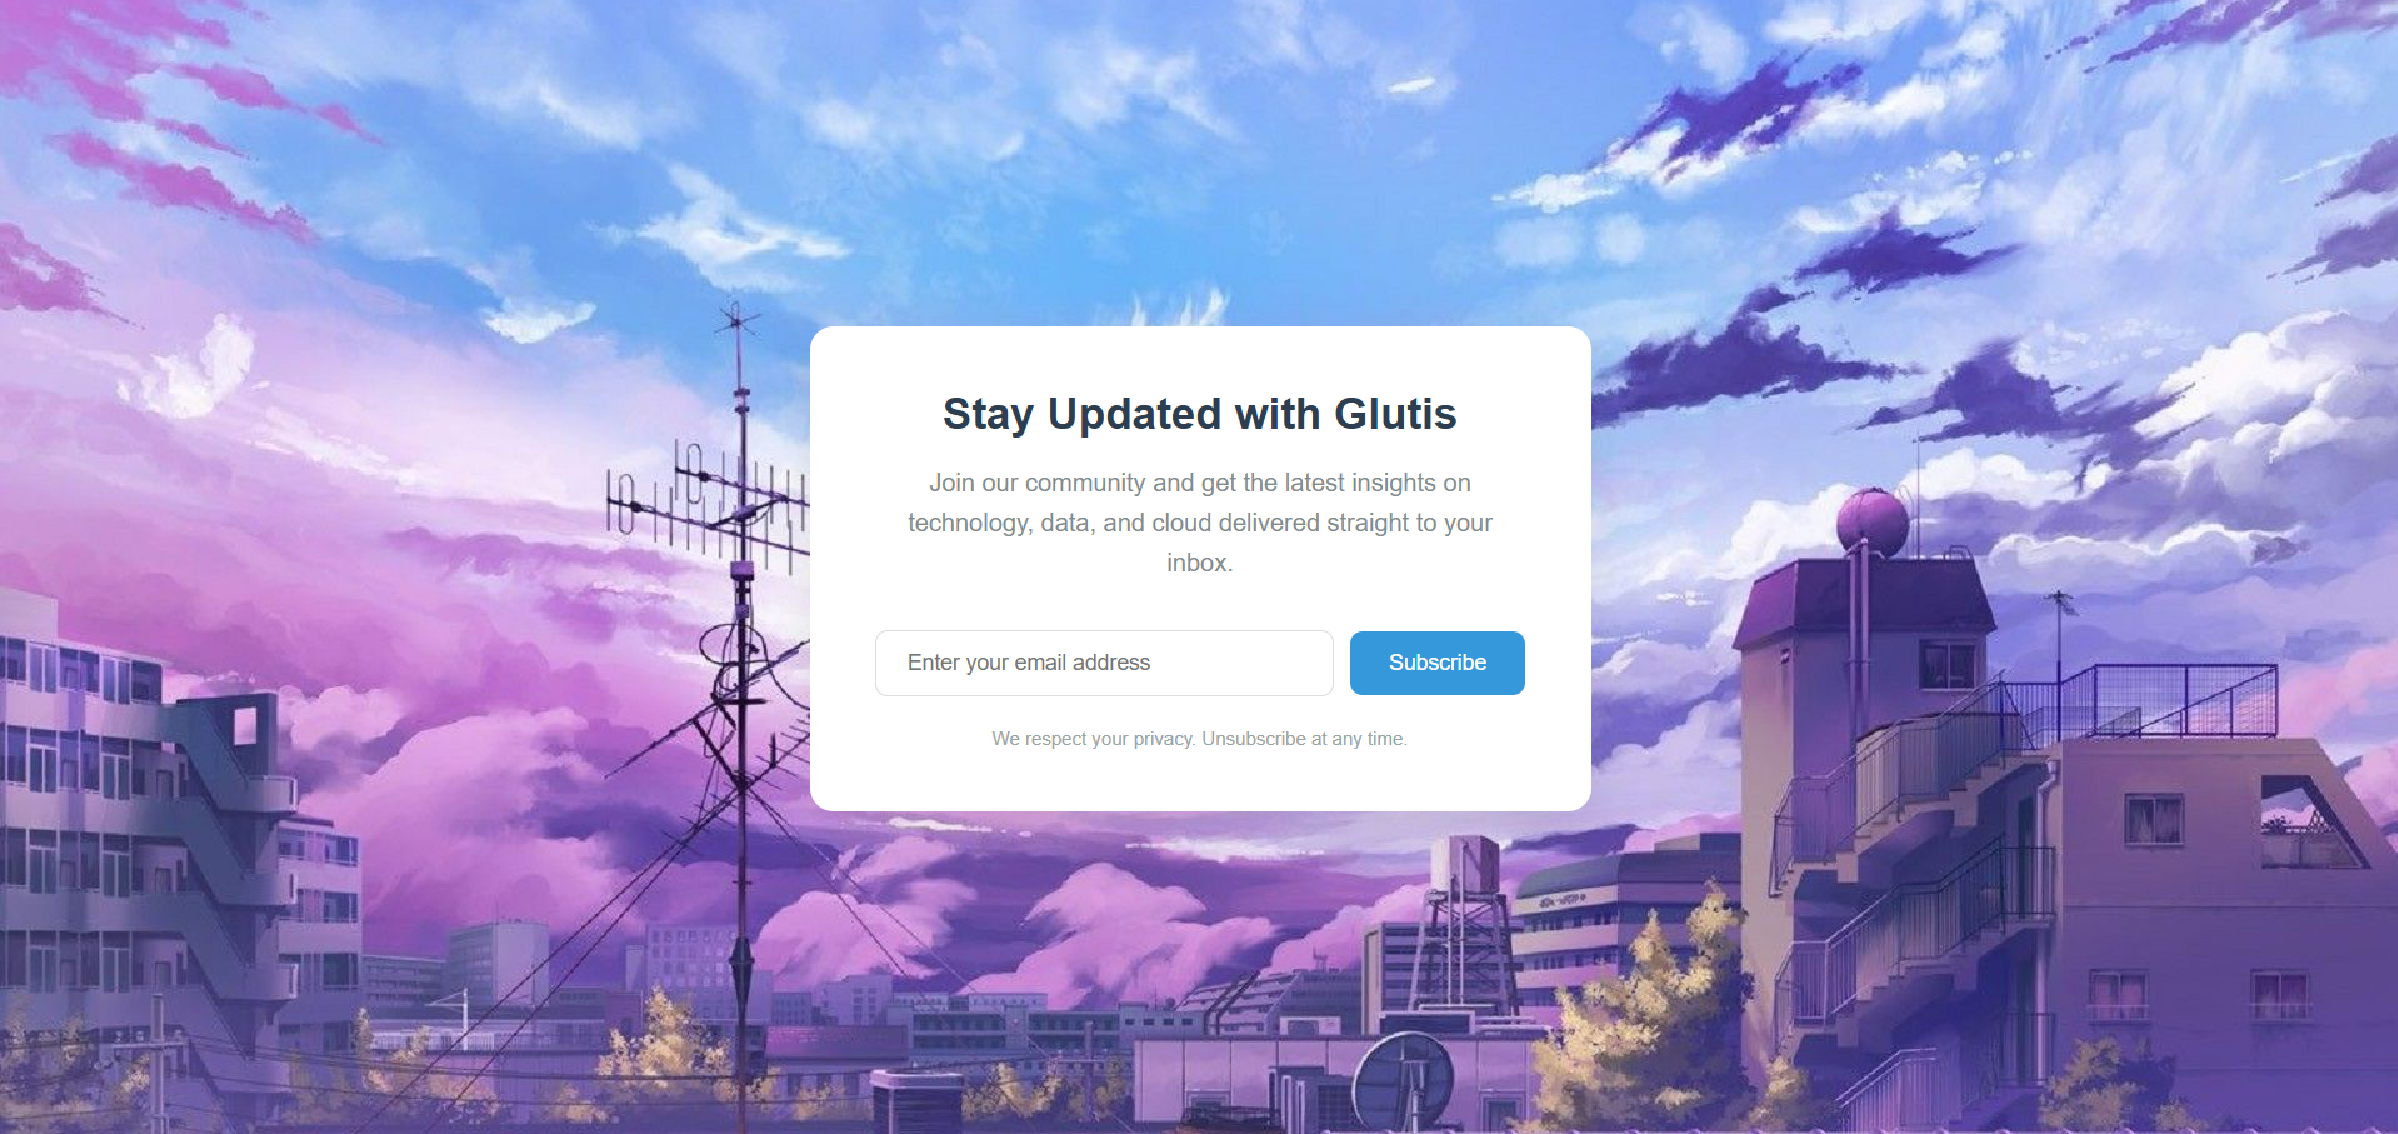
\includegraphics[width=1\linewidth]{Chap1-7/subscribe-page.pdf}
    \caption{Trang hướng người dùng đăng ký nhận thông tin}
\end{figure}

Mình viết một trang cho người dùng đăng ký bằng các nhập email cá nhân của họ. Sau khi người dùng nhập email của người dùng sẽ được điền vào google sheet thông qua App Scripts. Giao diện trang web được thiết kế đơn giản, thân thiện với người dùng, chỉ với một ô nhập liệu cho địa chỉ email và một nút nhấn để gửi thông tin đăng ký.


\newpage

\subsection{Các bước thực hiện}

Bước 1: Tạo Google Sheet

- Mở Google Sheets và tạo một bảng tính mới.

\begin{figure}[htbp]
    \centering
    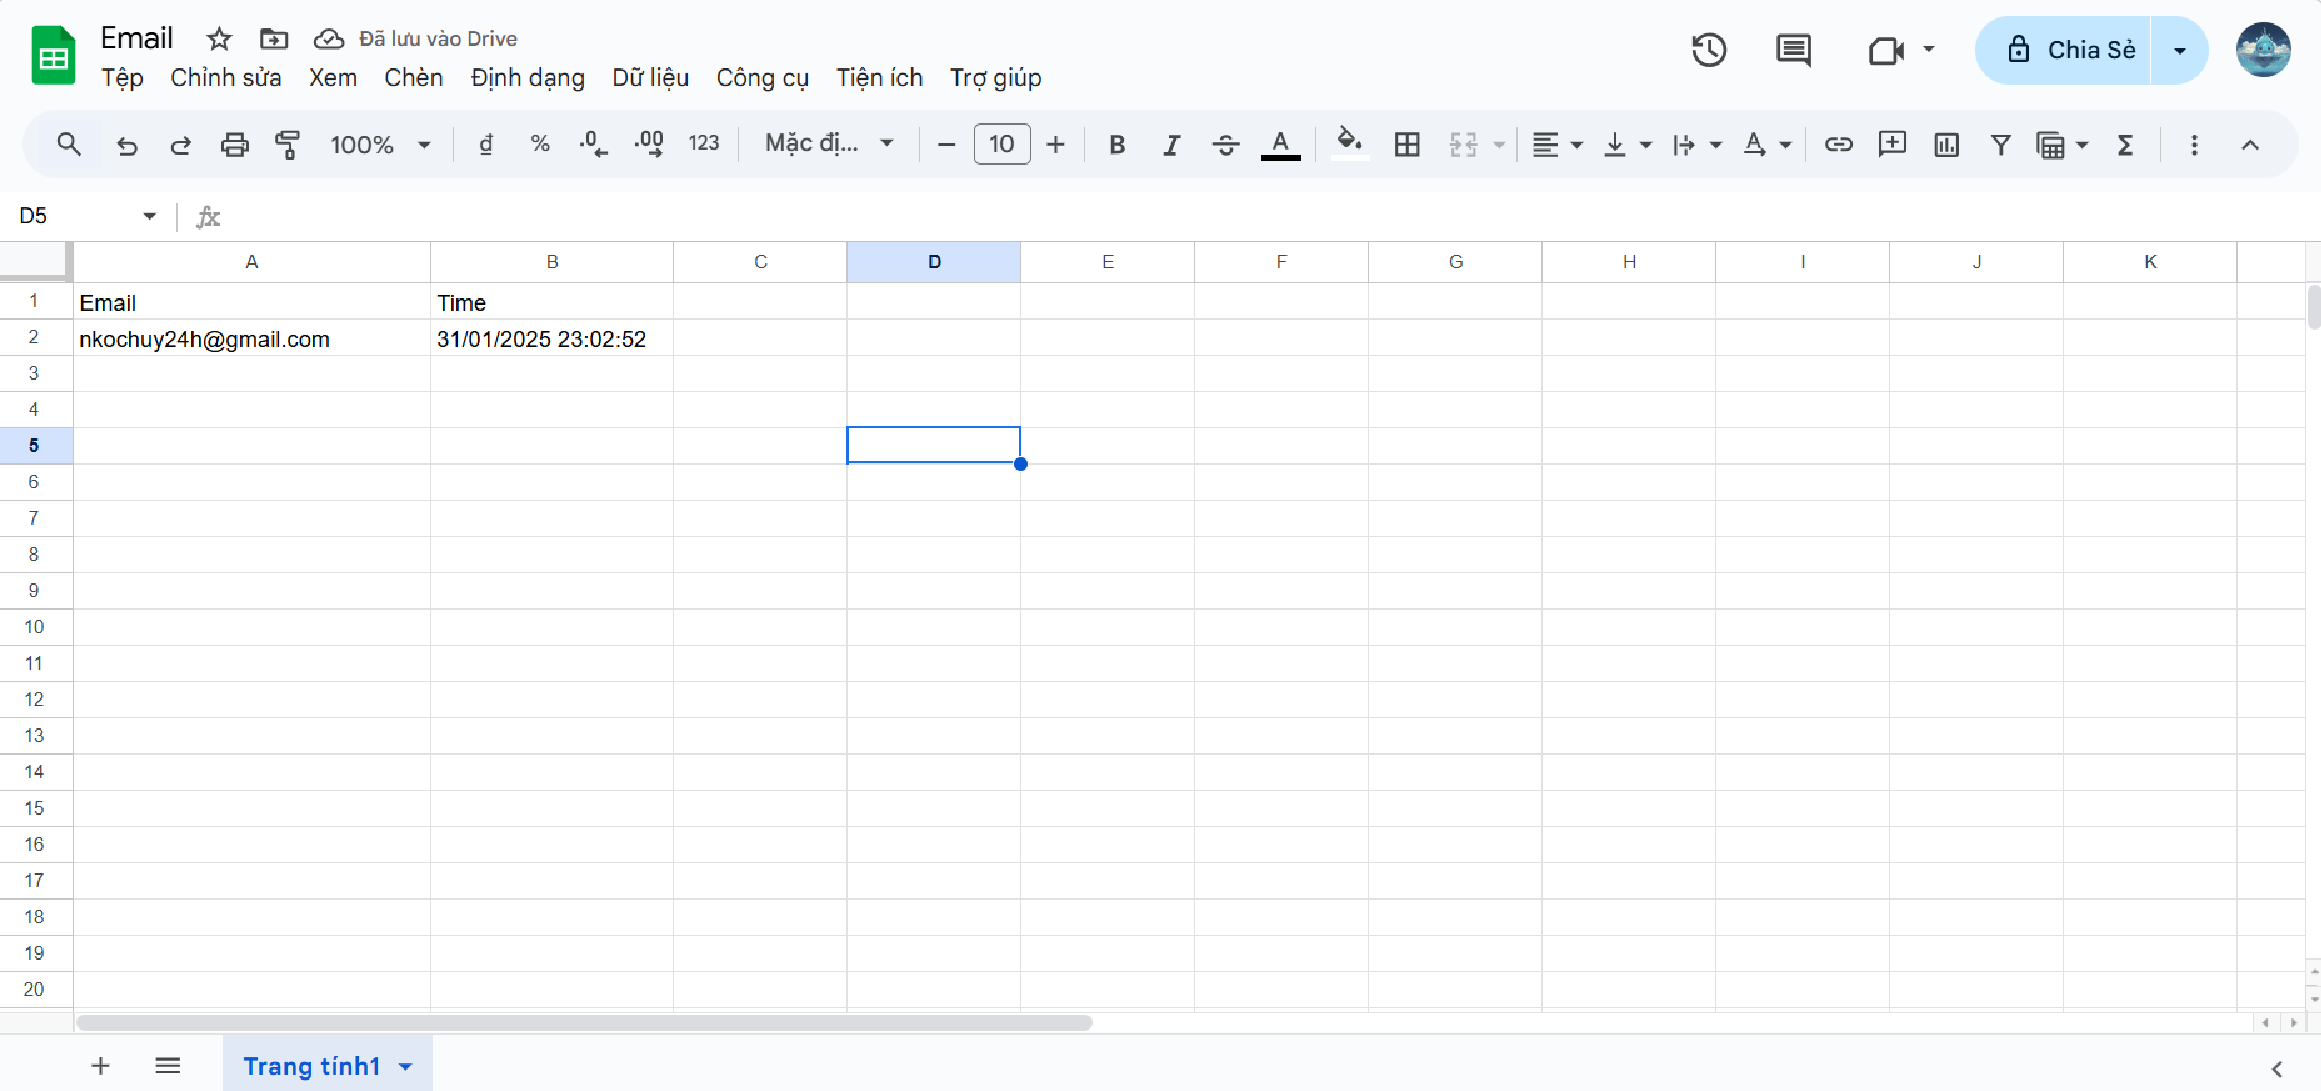
\includegraphics[width=1\linewidth]{Chap1-7/sheet_email.pdf}
\end{figure}

- Đặt tiêu đề cho cột A là Email.

- Chọn tiện ích và mở App Scripts tra một trang mới

- Copy lệnh dưới đây vào

\begin{verbatim}
function doPost(e) {
  const sheet = SpreadsheetApp.getActiveSpreadsheet().getActiveSheet();
  const formData = e.parameter; // Use e.parameter to get form data
  
  // Log the received email
  console.log('Received email:', formData.email);
  
  // Append the email to the sheet
  sheet.appendRow([formData.email, new Date()]); // Optional: also log timestamp
  
  return ContentService.createTextOutput(JSON.stringify({ result: 'success' }))
    .setMimeType(ContentService.MimeType.JSON);
}
\end{verbatim}

Bước 3: Triển khai Google Apps Script

\begin{figure}[htbp]
    \centering
    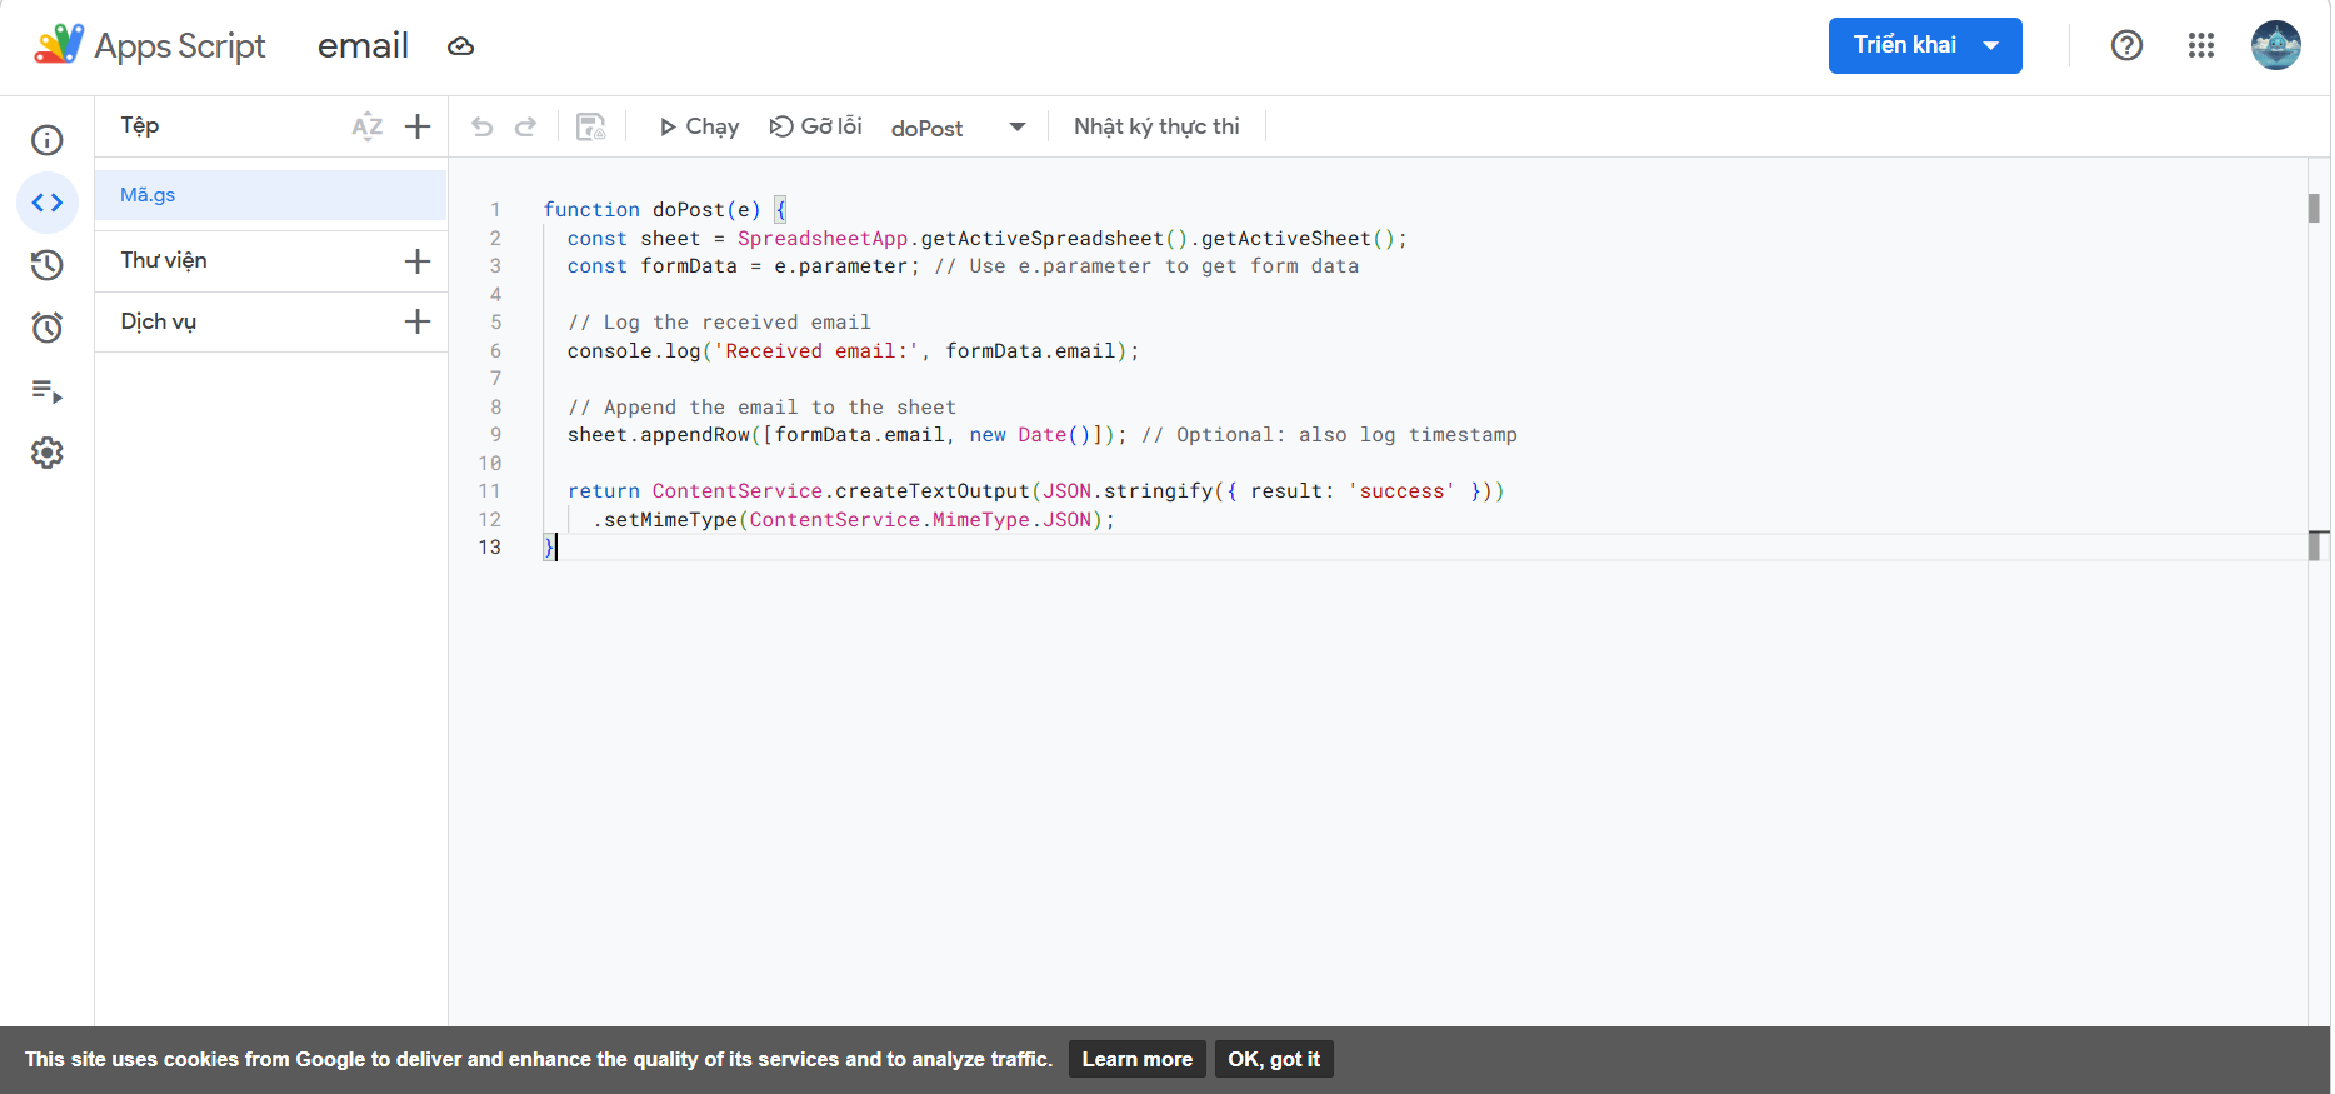
\includegraphics[width=1\linewidth]{Chap1-7/AppScripts.pdf}
\end{figure}

- Trong Google Apps Script, vào Deploy > New Deployment.

- Chọn Type: Web app.

- Chọn Who has access: Anyone (cho phép bên ngoài gửi request).

- Nhấn Deploy, cấp quyền và lấy URL của Web App.

Bước 4: Tạo trang HTML để nhập email

Tạo một file index.html với nội dung sau:

\begin{lstlisting}[language = HTML]
<!DOCTYPE html>
<html lang="en">
<head>
    <meta charset="UTF-8">
    <meta name="viewport" content="width=device-width, initial-scale=1.0">
    <title>Subscribe to Glutis</title>
    <link rel="stylesheet" href="style.css">
    <link rel="icon" type="image/png" href="images/icon-newsSubscribe.pdf">
</head>
<body>
    <div class="subscribe-container">
        <div class="subscribe-content">
            <h1>Stay Updated with Glutis</h1>
            <p class="subtitle">Join our community and get the latest insights on technology, data, and cloud delivered straight to your inbox.</p>
            
            <form name="submit-to-google-sheet">
                <div class="input-group">
                    <input type="email" name="email" placeholder="Enter your email address" required>

                    <button type="submit">Subscribe</button>
                </div>
            </form>

            <p class="disclaimer">We respect your privacy. Unsubscribe at any time.</p>
            <span id="msg" class="message"></span>
        </div>
    </div>

    <script>
        const scriptURL = 'https://script.google.com/macros/s/AKfycbxqYcEJfxatmSPbBaNdiR8XOfWrTJjOYYLiPxeeo4Xton24qq2IQrHCHuEYG8Bgcbm5/exec';
        const form = document.forms['submit-to-google-sheet'];
        const messageDiv = document.getElementById('msg');
        const submitBtn = form.querySelector('button[type="submit"]');

        function showMessage(text, type) {
            messageDiv.textContent = text;
            messageDiv.className = `message ${type}`;
            messageDiv.style.display = 'block';
            
            setTimeout(() => {
                messageDiv.style.display = 'none';
            }, 5000);
        }

        form.addEventListener('submit', async (e) => {
            e.preventDefault();
            
            submitBtn.textContent = 'Submitting...';
            submitBtn.disabled = true;

            try {
                const response = await fetch(scriptURL, {
                    method: 'POST',
                    mode: 'no-cors', 
                    body: new FormData(form)
                });
                showMessage('Success! Check your inbox for confirmation.', 'success');
                form.reset();
            } catch (error) {
                console.error('Error:', error);
                showMessage('Oops! Please try again later.', 'error');
            } finally {
                submitBtn.textContent = 'Subscribe';
                submitBtn.disabled = false;
            }
        });
    </script>
</body>
</html>
\end{lstlisting}

Thay thế scriptURL bằng URL copy ở bước trên, còn CSS thì mọi người tự custom nha :))

Bước 5: Tạo workflow trong n8n

- Tạo node schedule để đặt lịch chạy hăng ngày

- Cào dữ liệu từ trang blog cá nhân có thể sử dụng trực tiếp db của blog nếu muốn tuy nhiên để linh hoạt và tránh ảnh hưởng đến db hiện tại thì nên crawl trực tiếp do cấu trúc web cũng đơn giản

\begin{figure}[htbp]
    \centering
    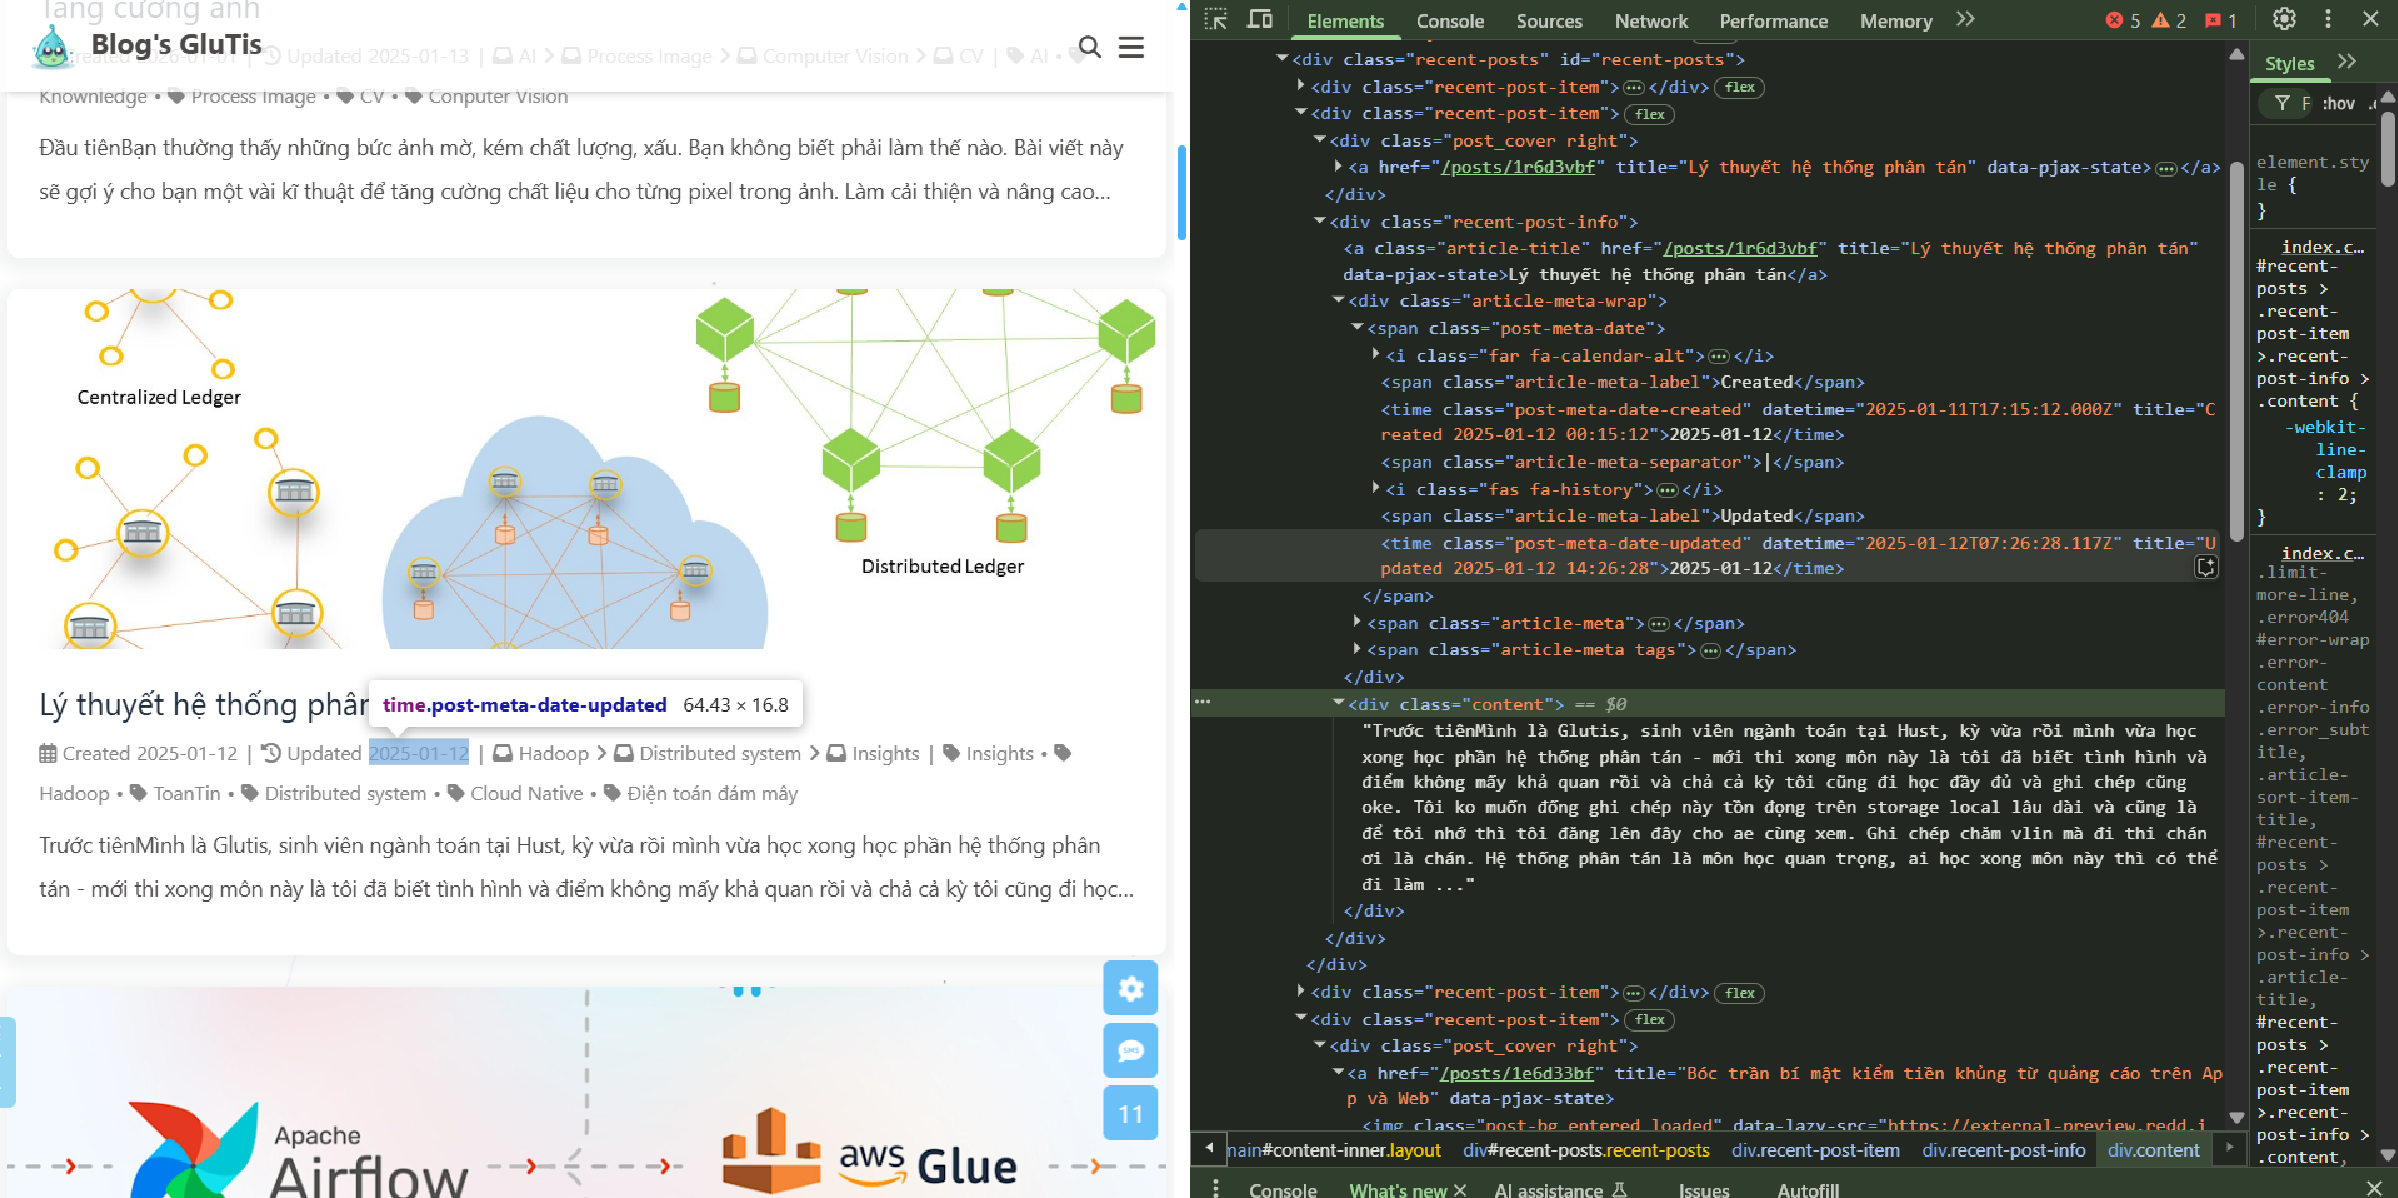
\includegraphics[width=1\linewidth]{Chap1-7/HTML_view.pdf}
    \caption{Xem mã nguồn HTML của trang}
\end{figure}

=> Với các Blog bất kỳ các bạn cứ F12 -> Copy đoạn html của trang xong paste vào cho chatGPT hỏi code để cào data rồi thêm vào node code

\newpage

- Chạy lần đầu để lưu các bài viết ở trang đầu vào nocodb.

\begin{figure}[htbp]
    \centering
    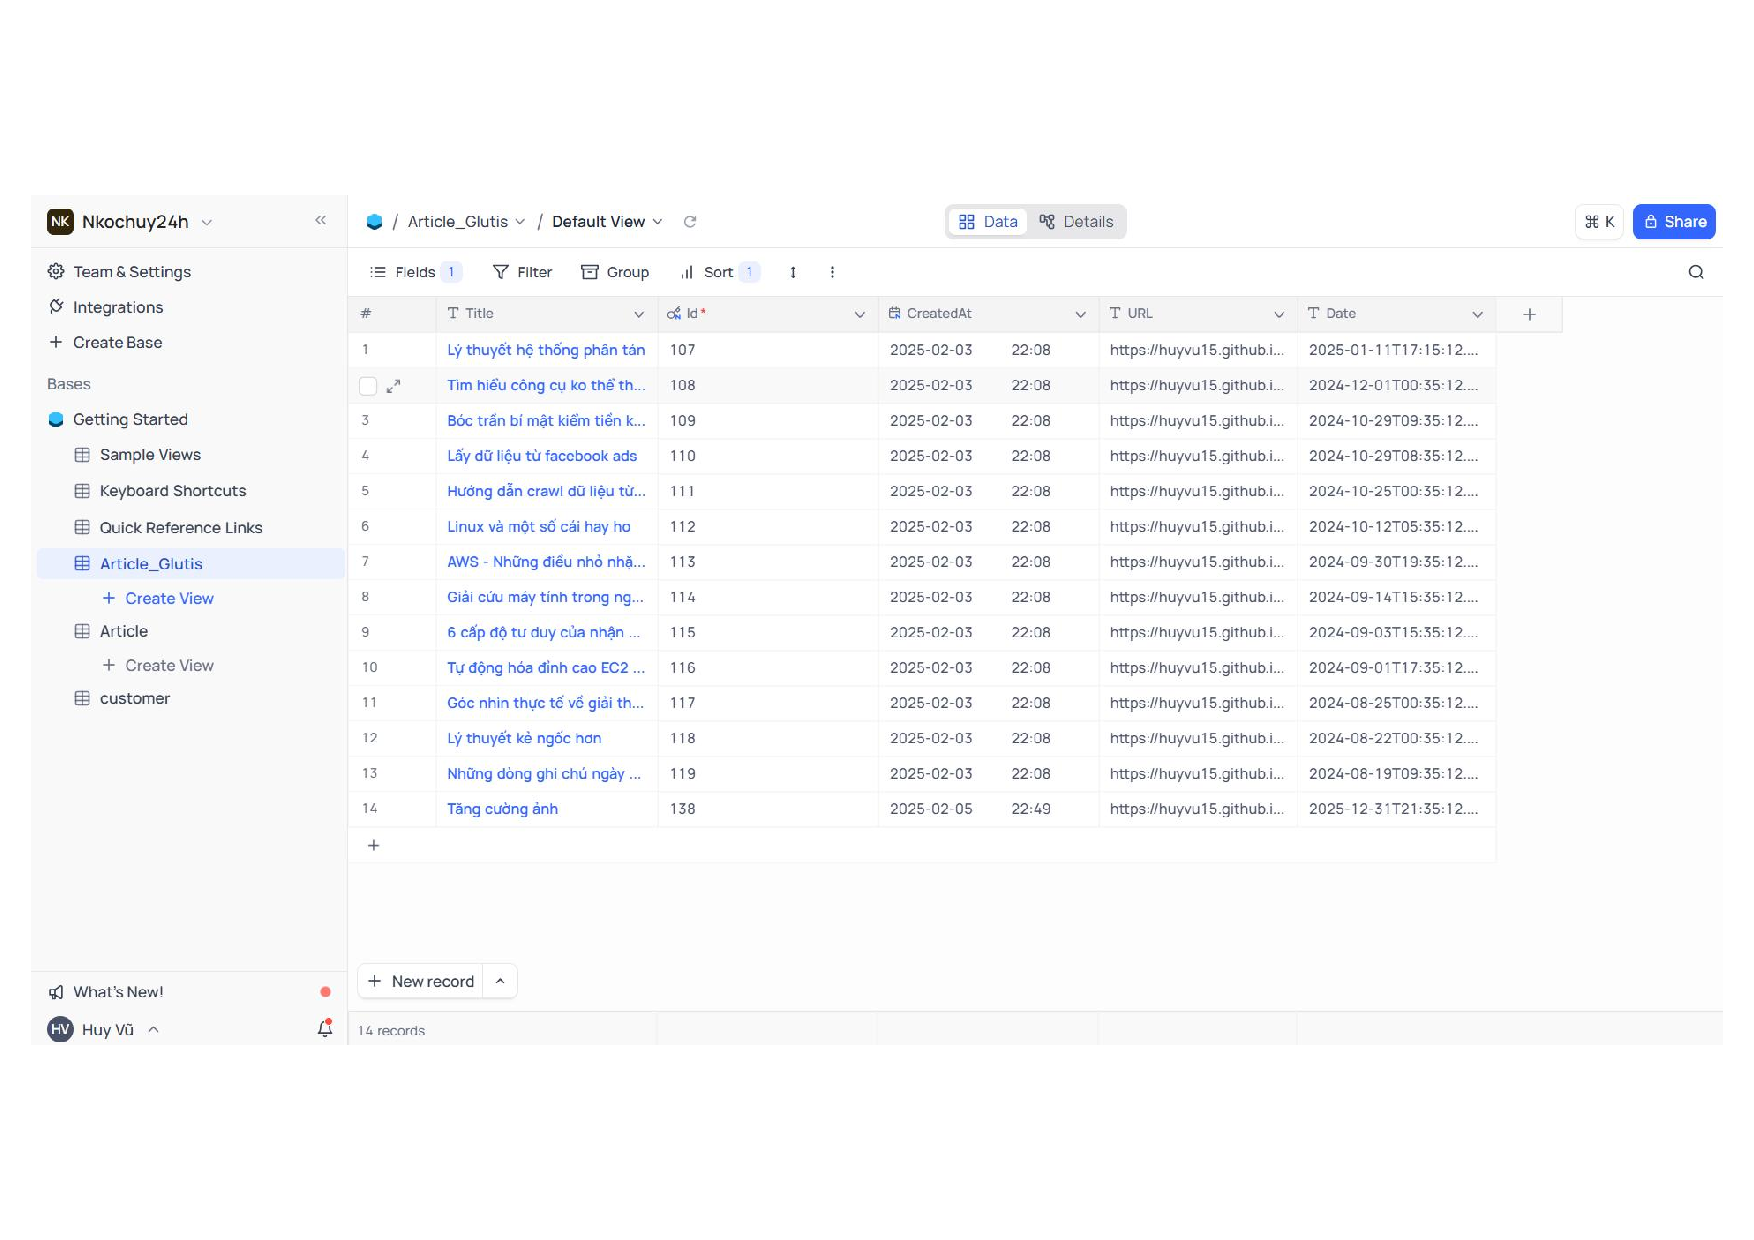
\includegraphics[width=1\linewidth]{Chap1-7/nocodb-article.pdf}
    \caption{Chỉ cào các bản ghi ở trang đầu Blog}
\end{figure}

- Các ngày tiếp theo tiếp tục cào. Thực hiện kiểm tra xem có bài viết mới hay không bằng cách so sánh id của bài viết với các bài viết trong db, nếu bài viết đã tồn tại thì end. Bài viết chưa tồn tại thì thêm bài viết đó vào nocodb sau đó chuyển bài viết đó thành dạng html do bài viết có lưu cả hình ảnh title, section. Mình muốn gửi cả bài viết đó qua email thì phải dùng dạng html và đường dẫn của ảnh cũng lưu vào db. 

\begin{figure}[htbp]
    \centering
    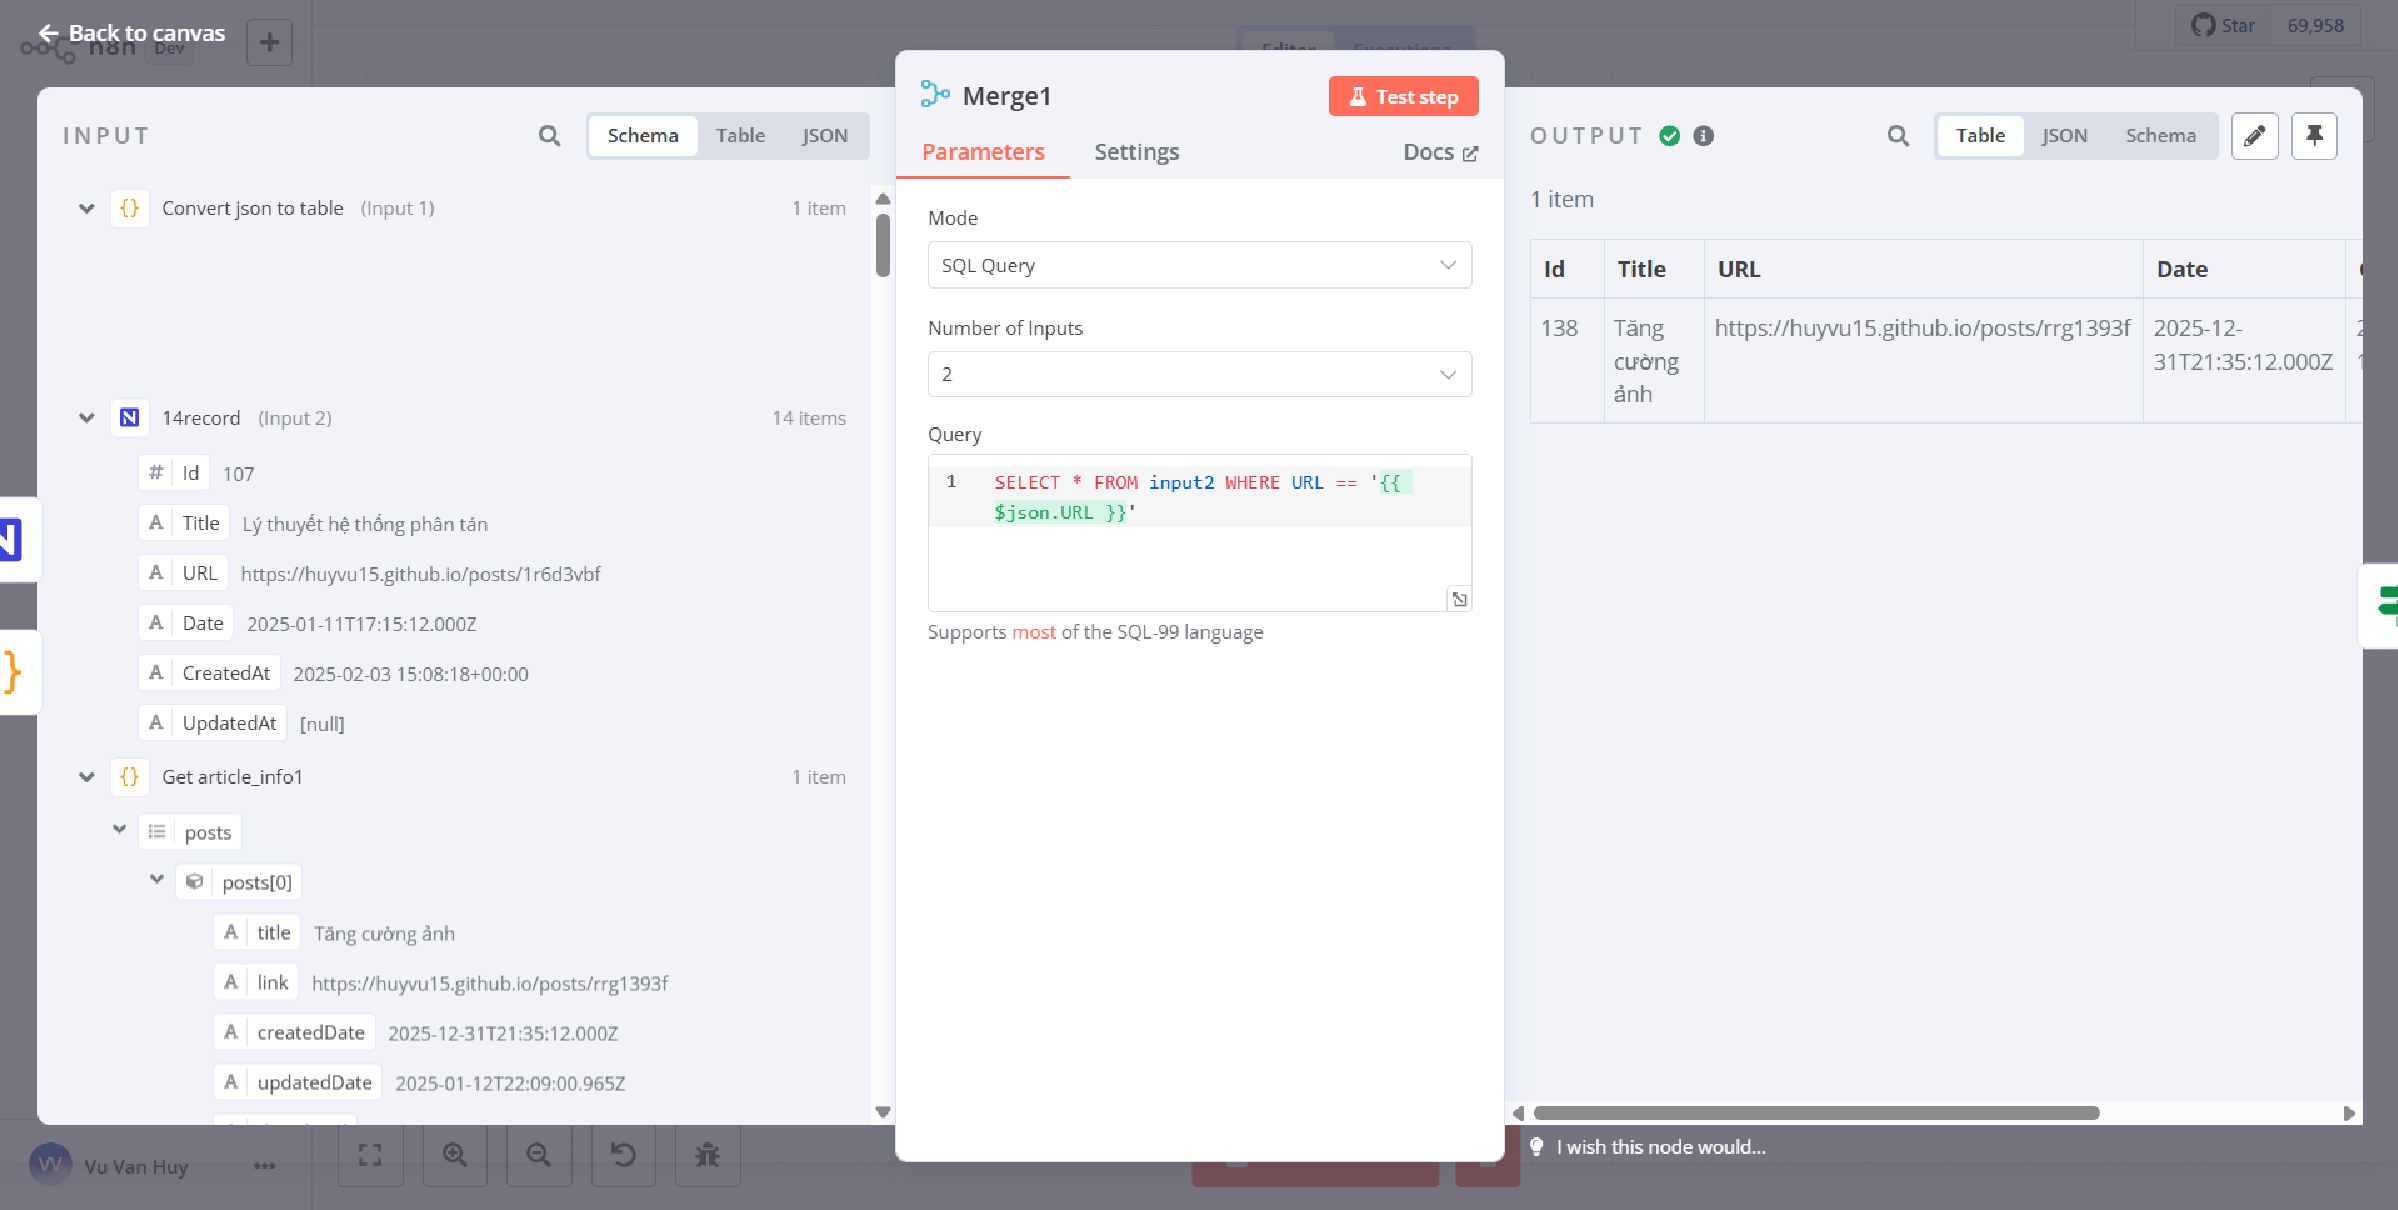
\includegraphics[width=1\linewidth]{Chap1-7/merge-project.pdf}
\end{figure}

\newpage

- Thực hiện tiền xử lý cơ bản, để ra đoạn html sạch sau cùng

- Gọi tới sheet và lấy ra tất cả các email ( bước này bao gồm lọc trùng, count)

- Đưa tất cả email đó cùng với đoạn html vào node Merge để kết hợp nội dung

- Gửi bài viết cho từng email đăng ký bằng node "Send Email"

Hoàn hoàn có thể cải tiến bằng cách gửi qua telegram bằng webhook. Tuy nhiên đây là một dạng marketing nên mình nghĩ dùng Gmail sẽ hợp hơn

\newpage

\textbf{Kết quả: }

\begin{figure}[htbp]
    \centering
    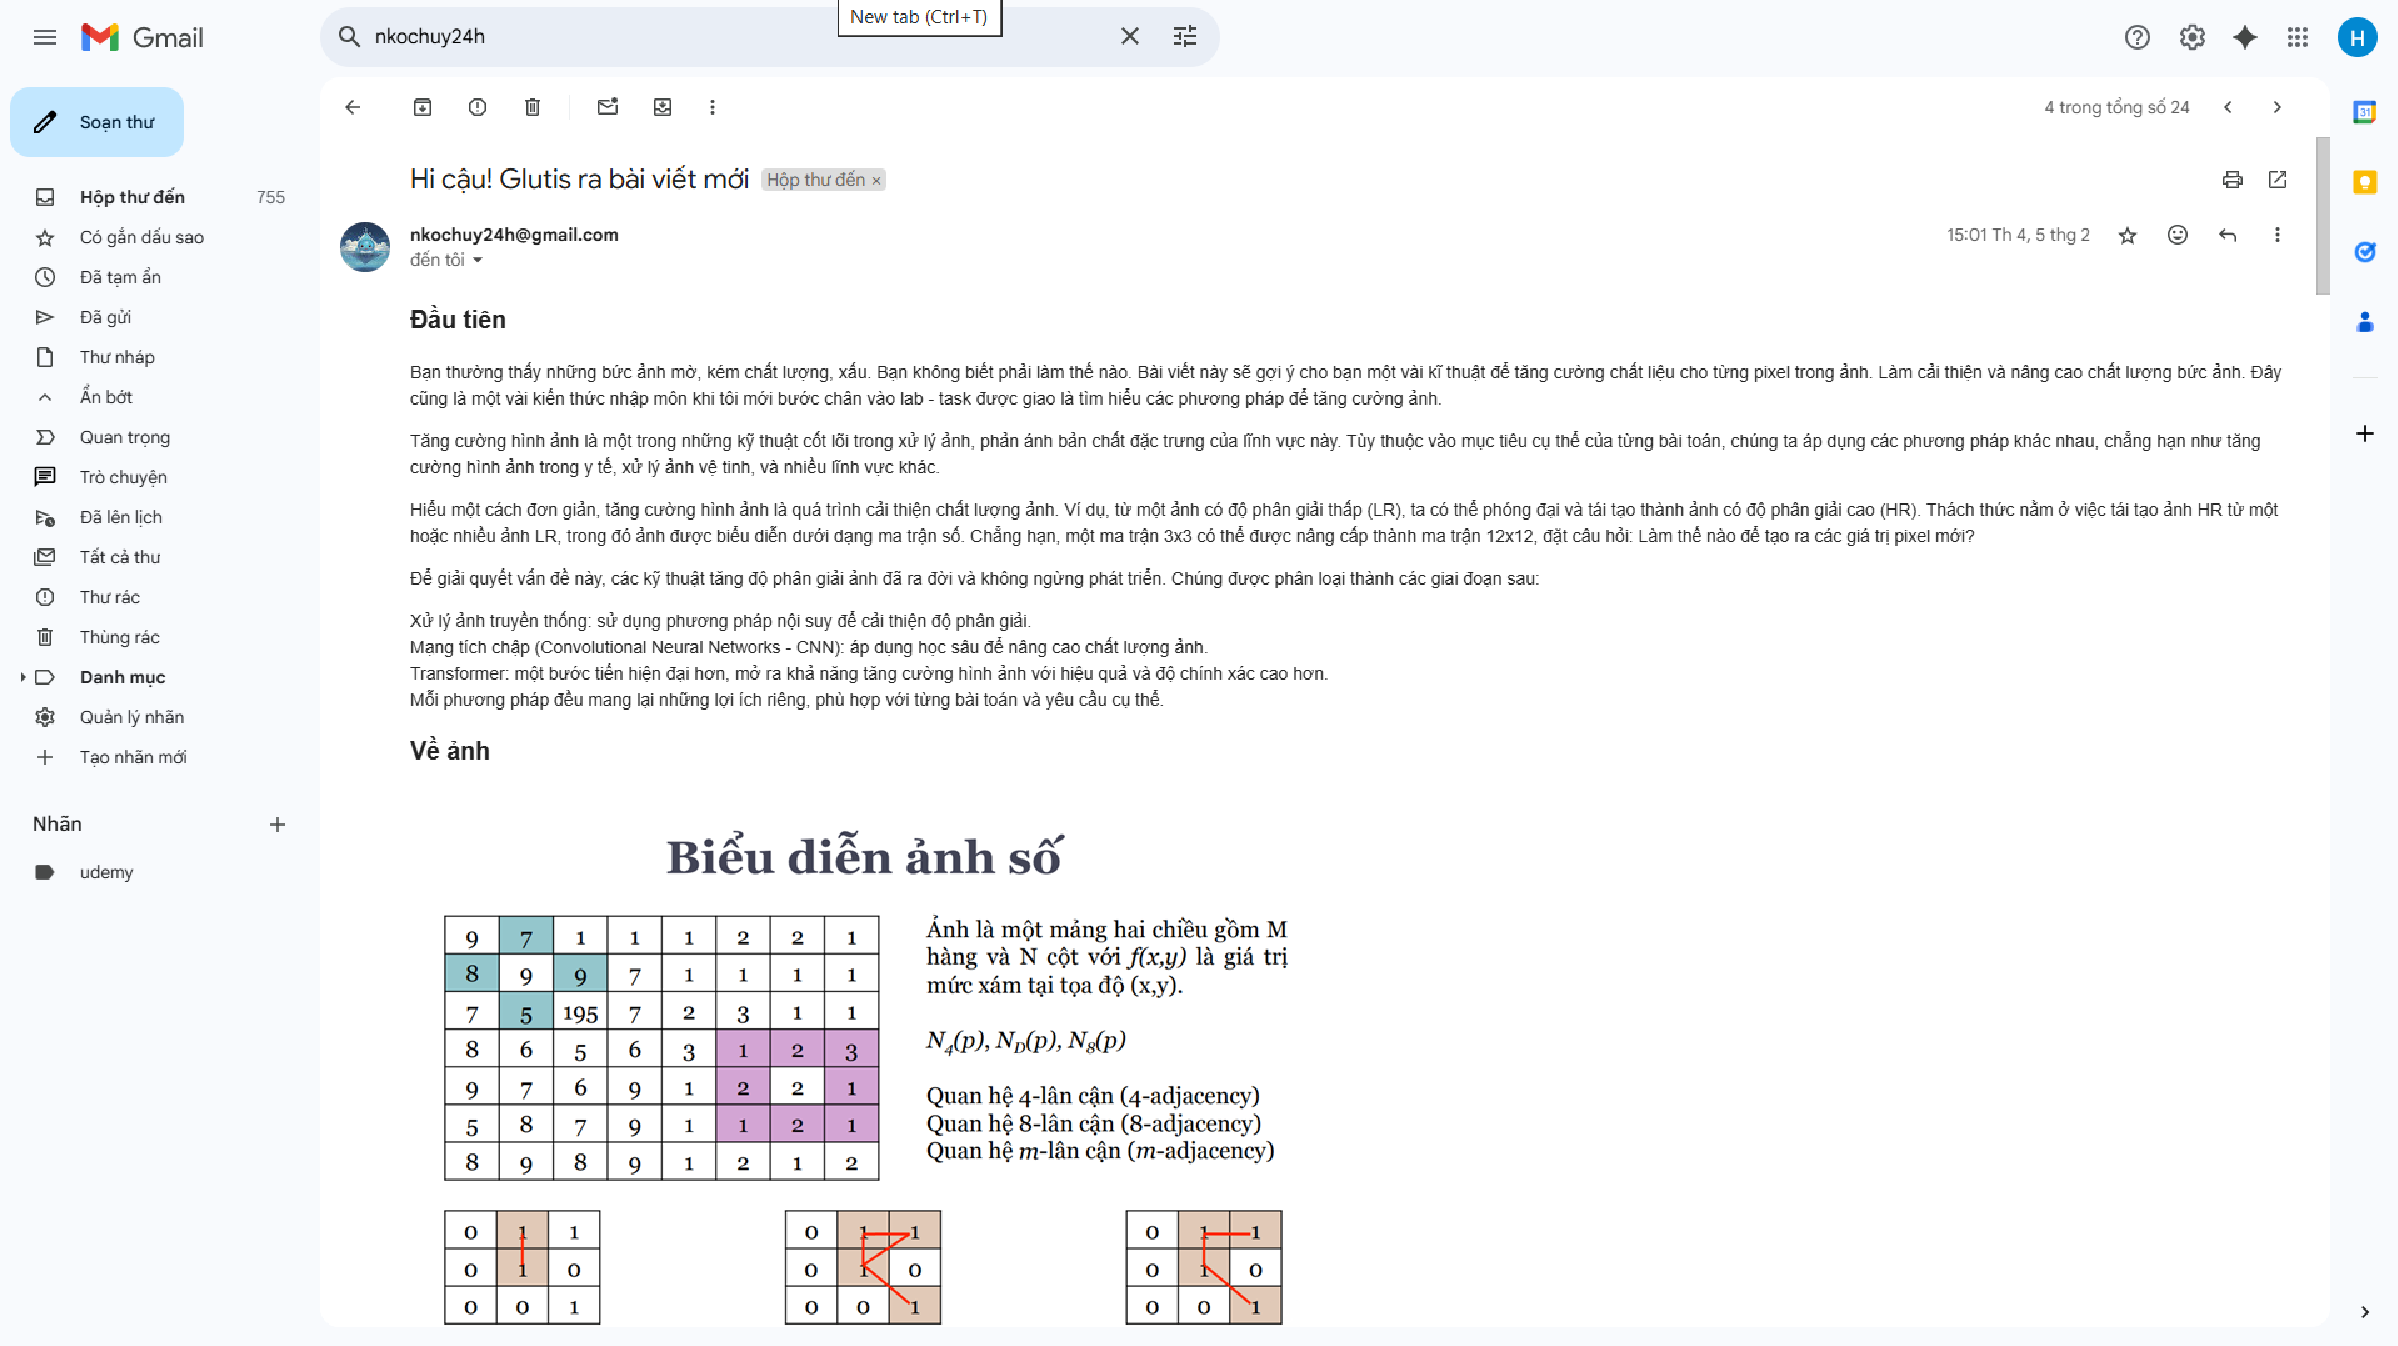
\includegraphics[width=1\linewidth]{Chap1-7/glutis-subcriber-results.pdf}
    \caption{Người đăng ký nhận được tin nhắn thông báo mỗi khi có bài viết mới}
\end{figure}

Mình vừa triển khai một hệ thống nhỏ để gửi thông báo bài viết mới cho blog cá nhân glutis.is-a.dev mà không cần can thiệp vào code của blog. Giải pháp này sử dụng:

\begin{itemize}
    \item Google Sheets + Apps Script: thu thập danh sách email.

    \item n8n: tự động crawl bài viết mới, xử lý dữ liệu và gửi email thông báo.
\end{itemize}

Kết quả:
\begin{itemize}
    \item Tiết kiệm kha khá thời gian kiểm tra và gửi tay.
    \item Độc giả luôn được cập nhật bài mới ngay trong hộp thư.
    \item  Hệ thống dễ mở rộng: tích hợp thêm thông báo qua Telegram, Discord, hay auto-post Facebook đều khả thi.
\end{itemize}

\textbf{Kinh nghiệm rút ra:}
Dùng công cụ no-code như n8n rất linh hoạt cho các tác vụ tự động nhỏ mà hiệu quả cao. Nếu bạn cũng muốn giữ kết nối với độc giả tốt hơn, thử cách này nhé!

\newpage 


\section{Dự án 5: Tự tạo bot thông minh phải hồi bình luận bài đăng và trả lời tin nhắn cho page bán vòng}

Mình có 1 page bán vòng có gì mọi người ủng hộ cho bà chủ kênh 
\href{fb.com}{Tiệm cái vòng nè} nha :))). Page mình thi thoảng mới có người để trực và trả lời các bình luận từ phía người dùng cùng như các tin nhắn khách hỏi. Đặc biệt các phản hồi và tin nhắn của người dùng thường xuyên diễn ra ngoài ra hành chính, có thể vào ban đêm rất khuya có ai đó hỏi tư vấn vòng tay thời trang. Do sức người có hạn nên mình nghĩ ra cái workflow này để giúp ích mình và bà chủ tiệm bán hàng cho hiệu quả.

\subsection{Phase 1: Tạo bot trả lời tin nhắn tự động dựa trên RAG}
\begin{figure}[htbp]
    \centering
    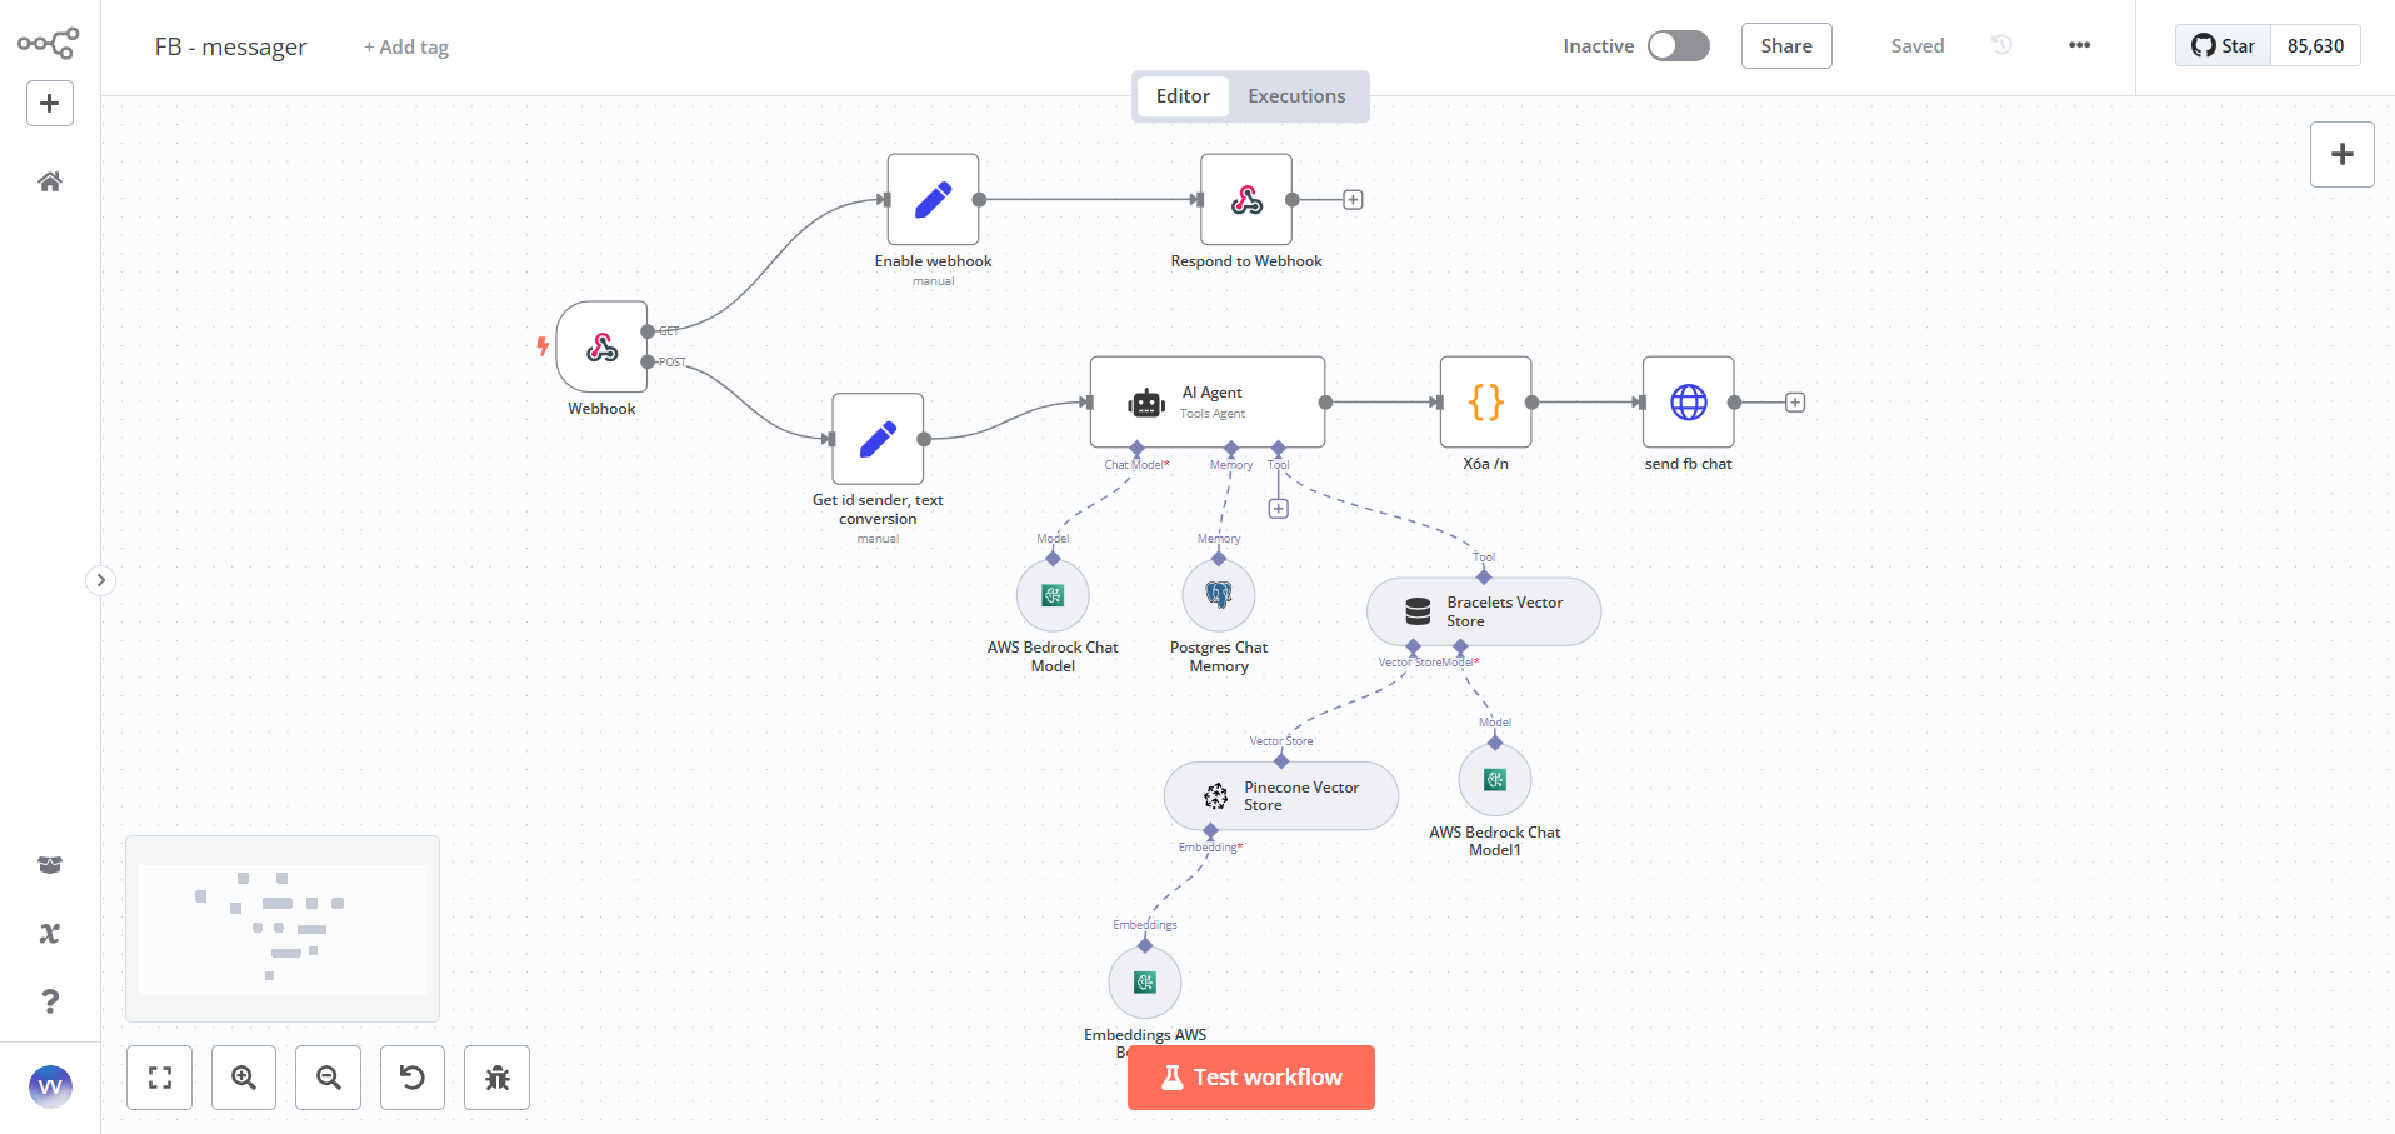
\includegraphics[width=1\linewidth]{Chap1-7/fb_mess.pdf}
    \caption{Tổng quan giải pháp}
\end{figure}

Khi khách hàng nhắn tin vào fanpage Facebook bán vòng tay, hệ thống sẽ tự động:

\begin{itemize}
    \item Nhận tin nhắn.

    \item Phân tích nội dung.

    \item Tư vấn hoặc trả lời khách dựa trên AI.

    \item Ghi lại lịch sử trò chuyện vào PostgreSQL.

    \item Tra cứu dữ liệu sản phẩm đã được embedding trong Pinecone.

    \item Trả lời lại khách hàng qua API Facebook.
\end{itemize}

$\rightarrow$ Các node Set để trích xuất thông tin như senderid và message.

\newpage

\begin{figure}[htbp]
    \centering
    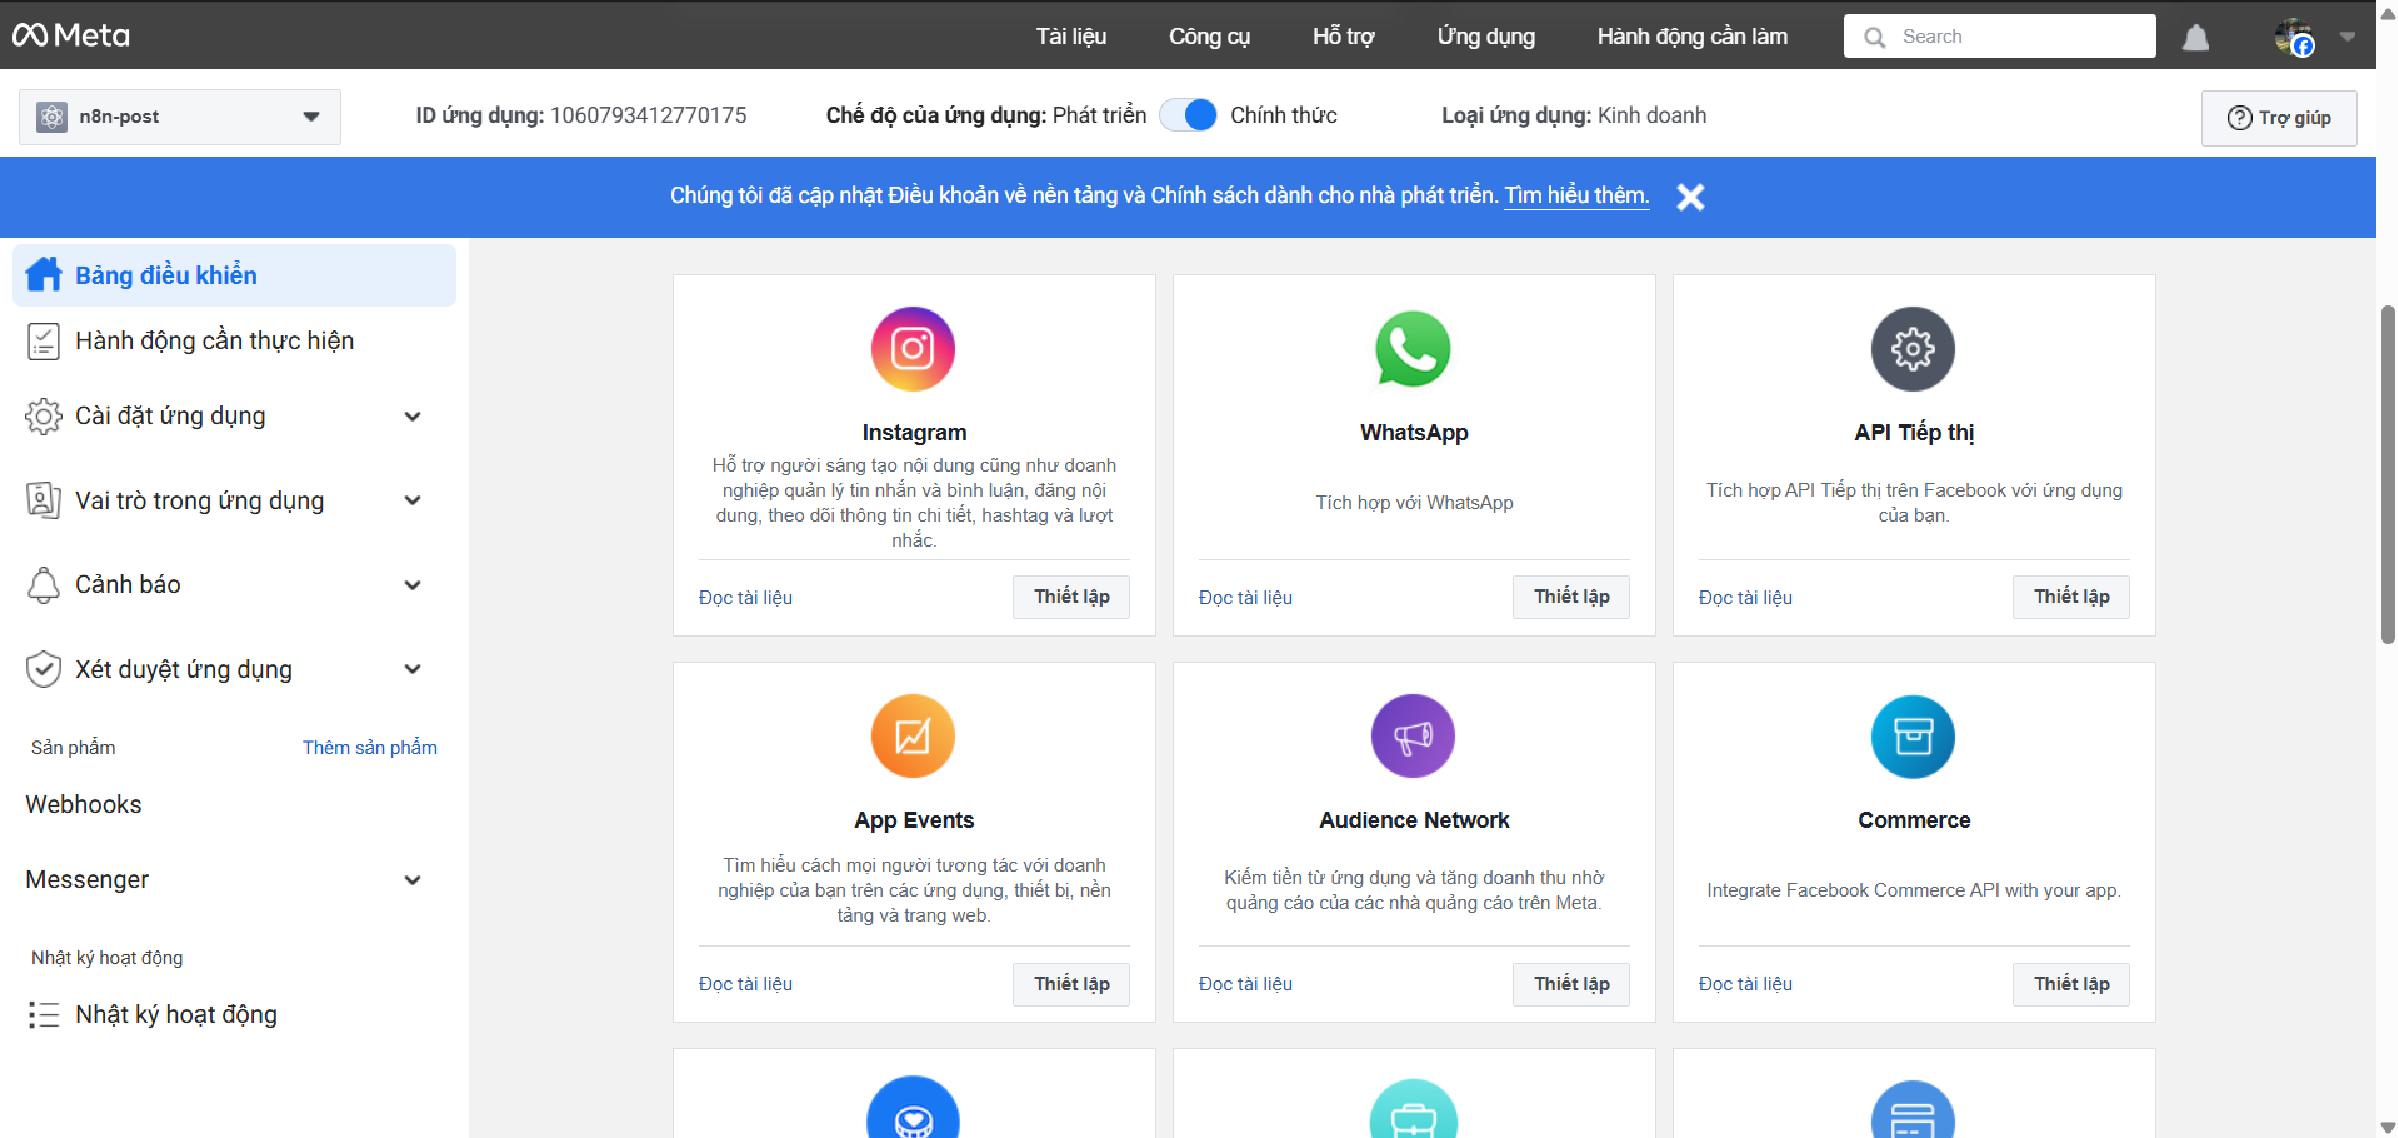
\includegraphics[width=1\linewidth]{Chap1-7/dev-fb.pdf}
\end{figure}

Trước tiên truy cập vào \href{https://developers.facebook.com/apps/}{https://developers.facebook.com/apps/}. Tạo một ứng dụng đặt tên là n8n-post. Truy cập vào giao diện chọn "Thêm sản phẩm". Tìm "Messager", "Webhook" chọn thiết lập xong thì nó sẽ hiện dưới chỗ sản phẩm như hình.

\begin{figure}[htbp]
    \centering
    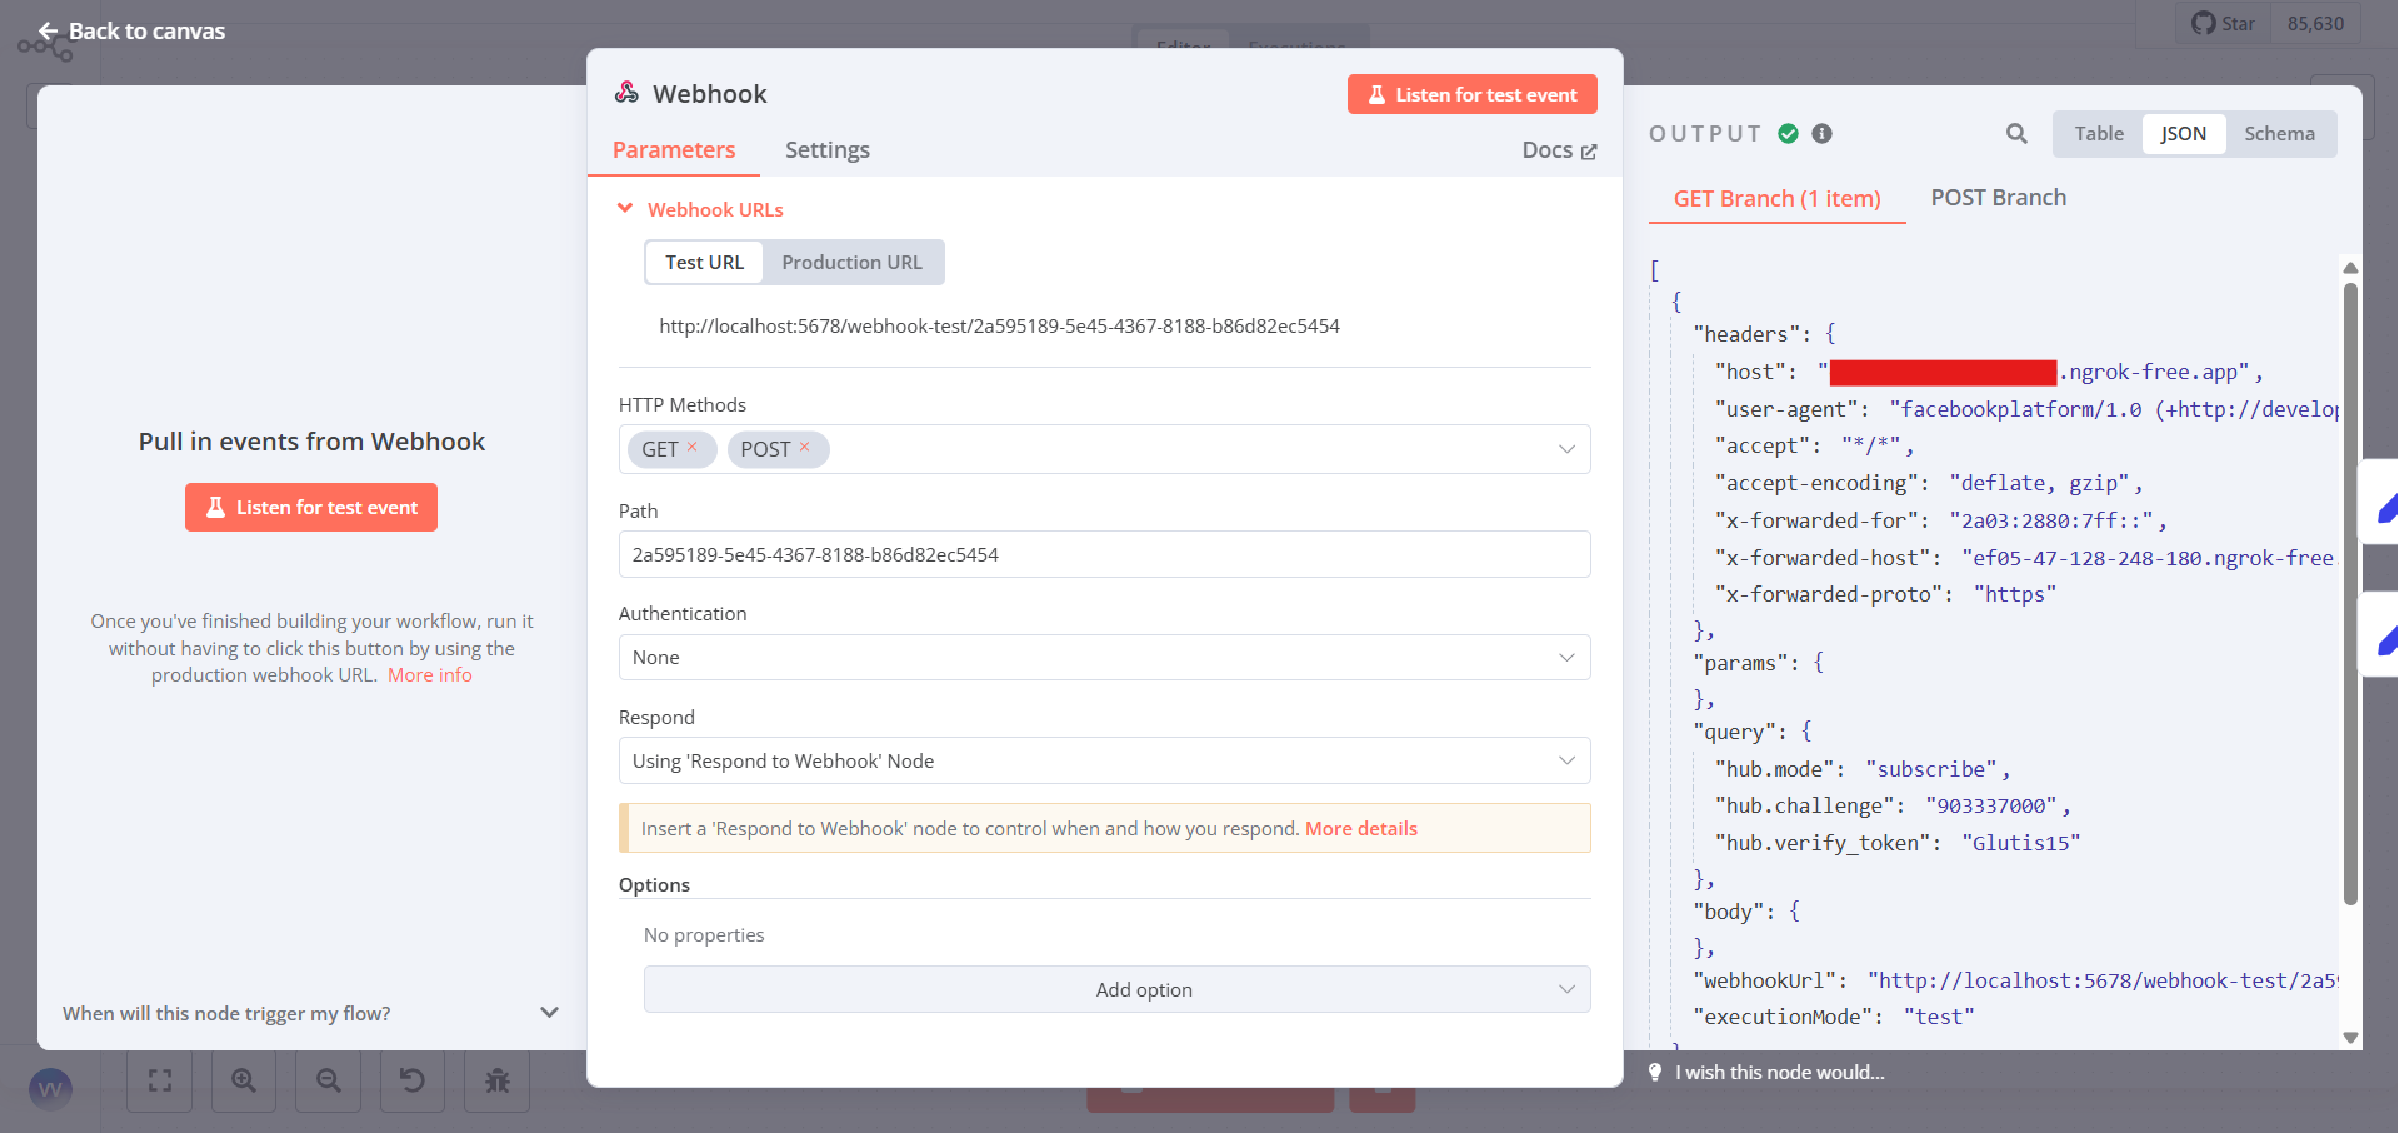
\includegraphics[width=1\linewidth]{Chap1-7/webhook1.pdf}
\end{figure}
- Tại nút webhook chọn Settings, bật Multiple HTTP Methods.

$\rightarrow$ Sẽ xuất hiện cả Post, GET cho 2 luồng

- Tại response chọn "Using Respond to Webhook Node"

- Điền đầy đủ thông tin bên trang dev của facebook.

- Bật webhook trên n8n, nhấn xác nhận ở trang dev

- Chọn quyền cho webhook là "messager". Cái này nên chọn đủ thôi nha, thừa là cx bị lỗi khi gửi messager đó.

\begin{figure}[htbp]
    \centering
    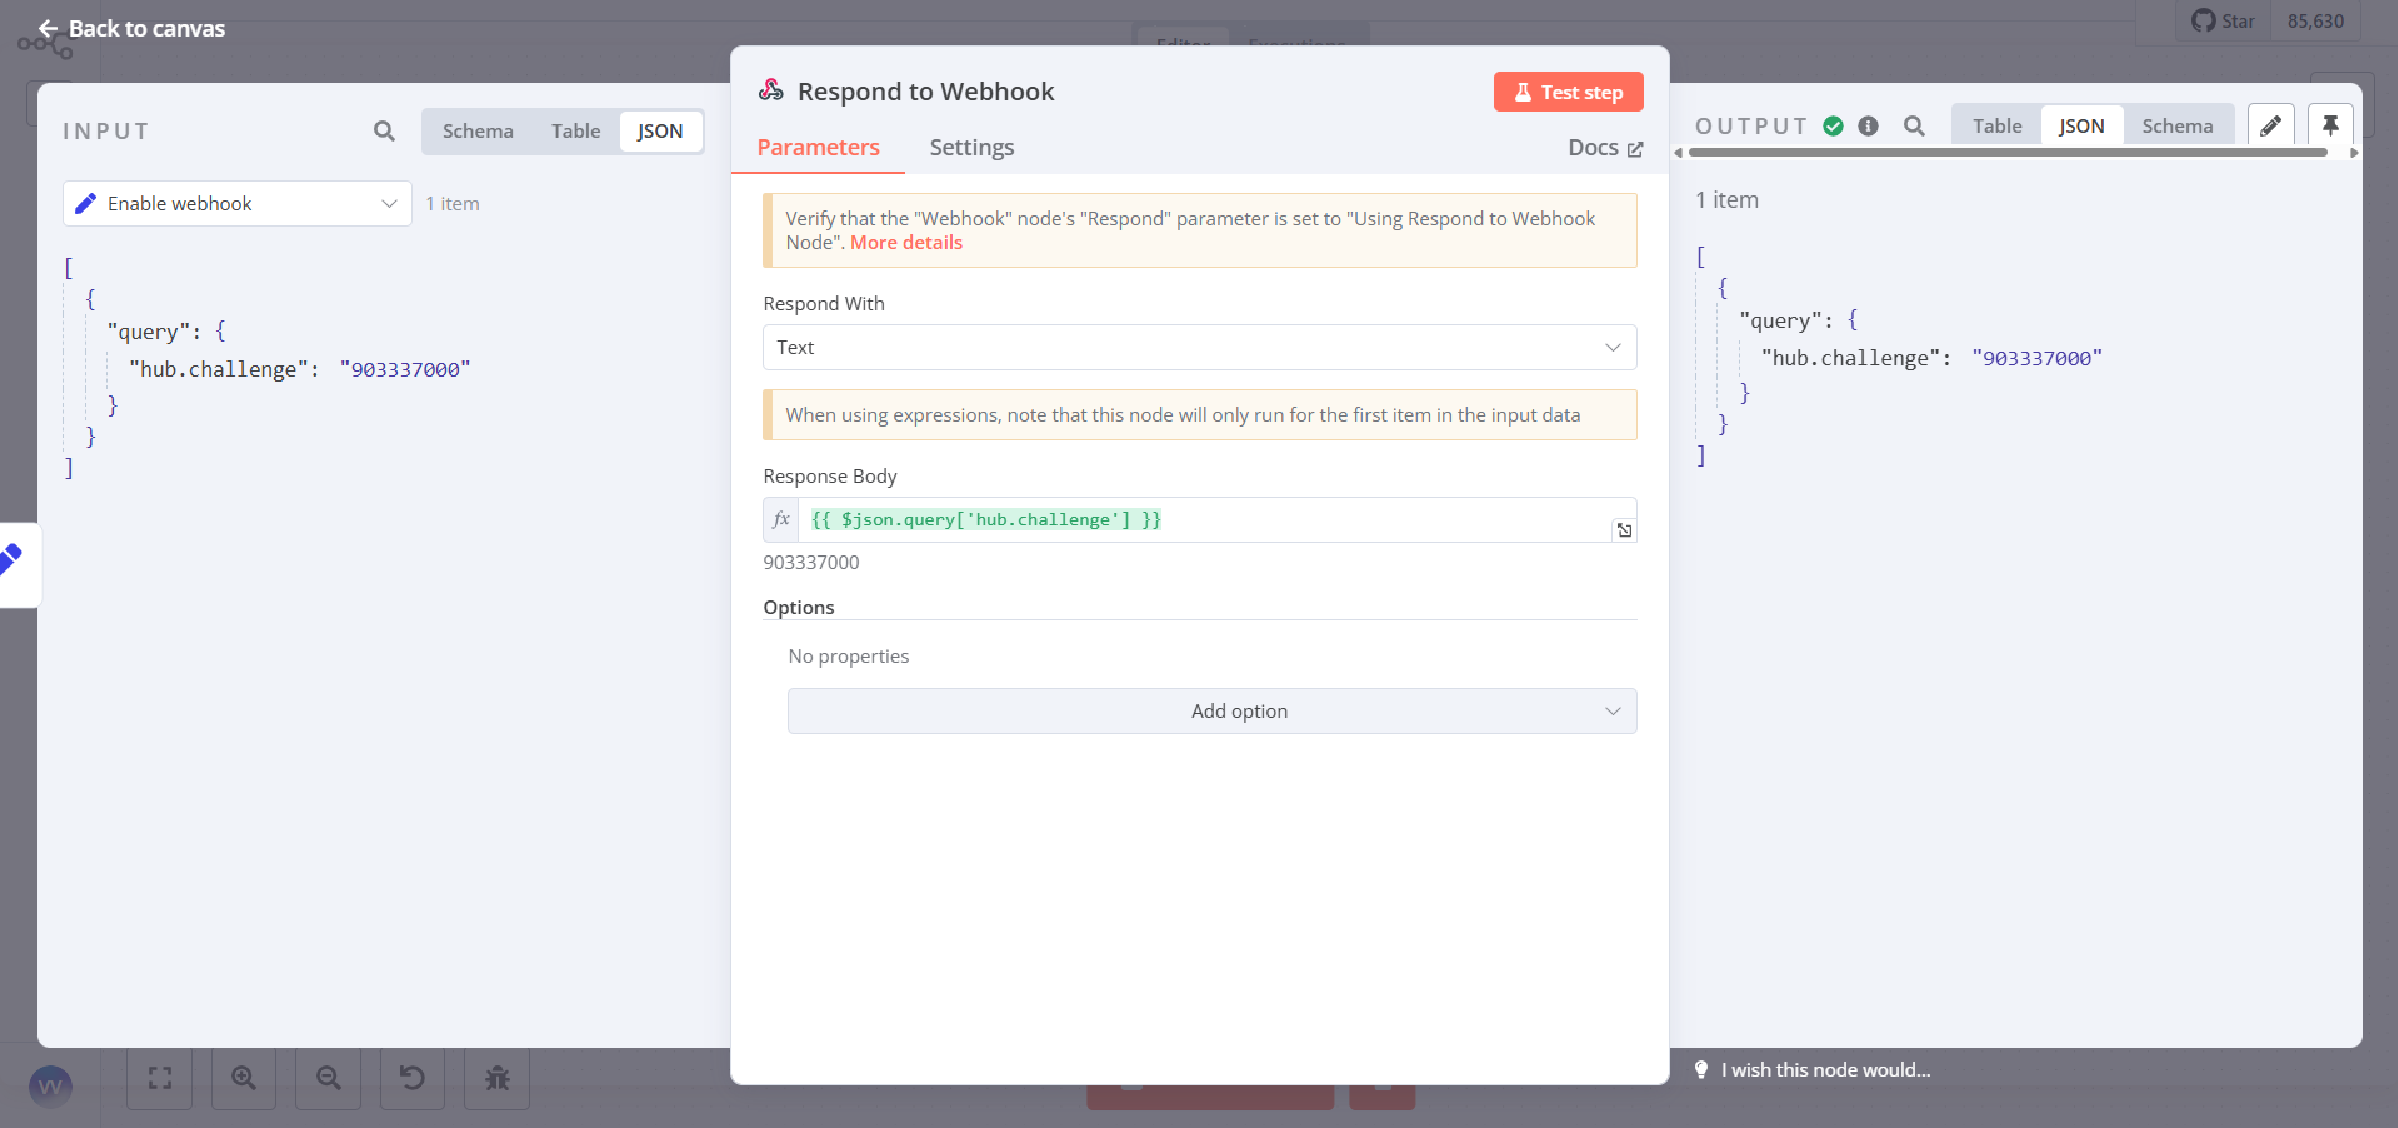
\includegraphics[width=1\linewidth]{Chap1-7/webhook2.pdf}
\end{figure}

- Tại node Respone to Webhook kéo phần hub.challenge vào đây để phản hồi lại cho sever của facebook.


\begin{figure}[htbp]
    \centering
    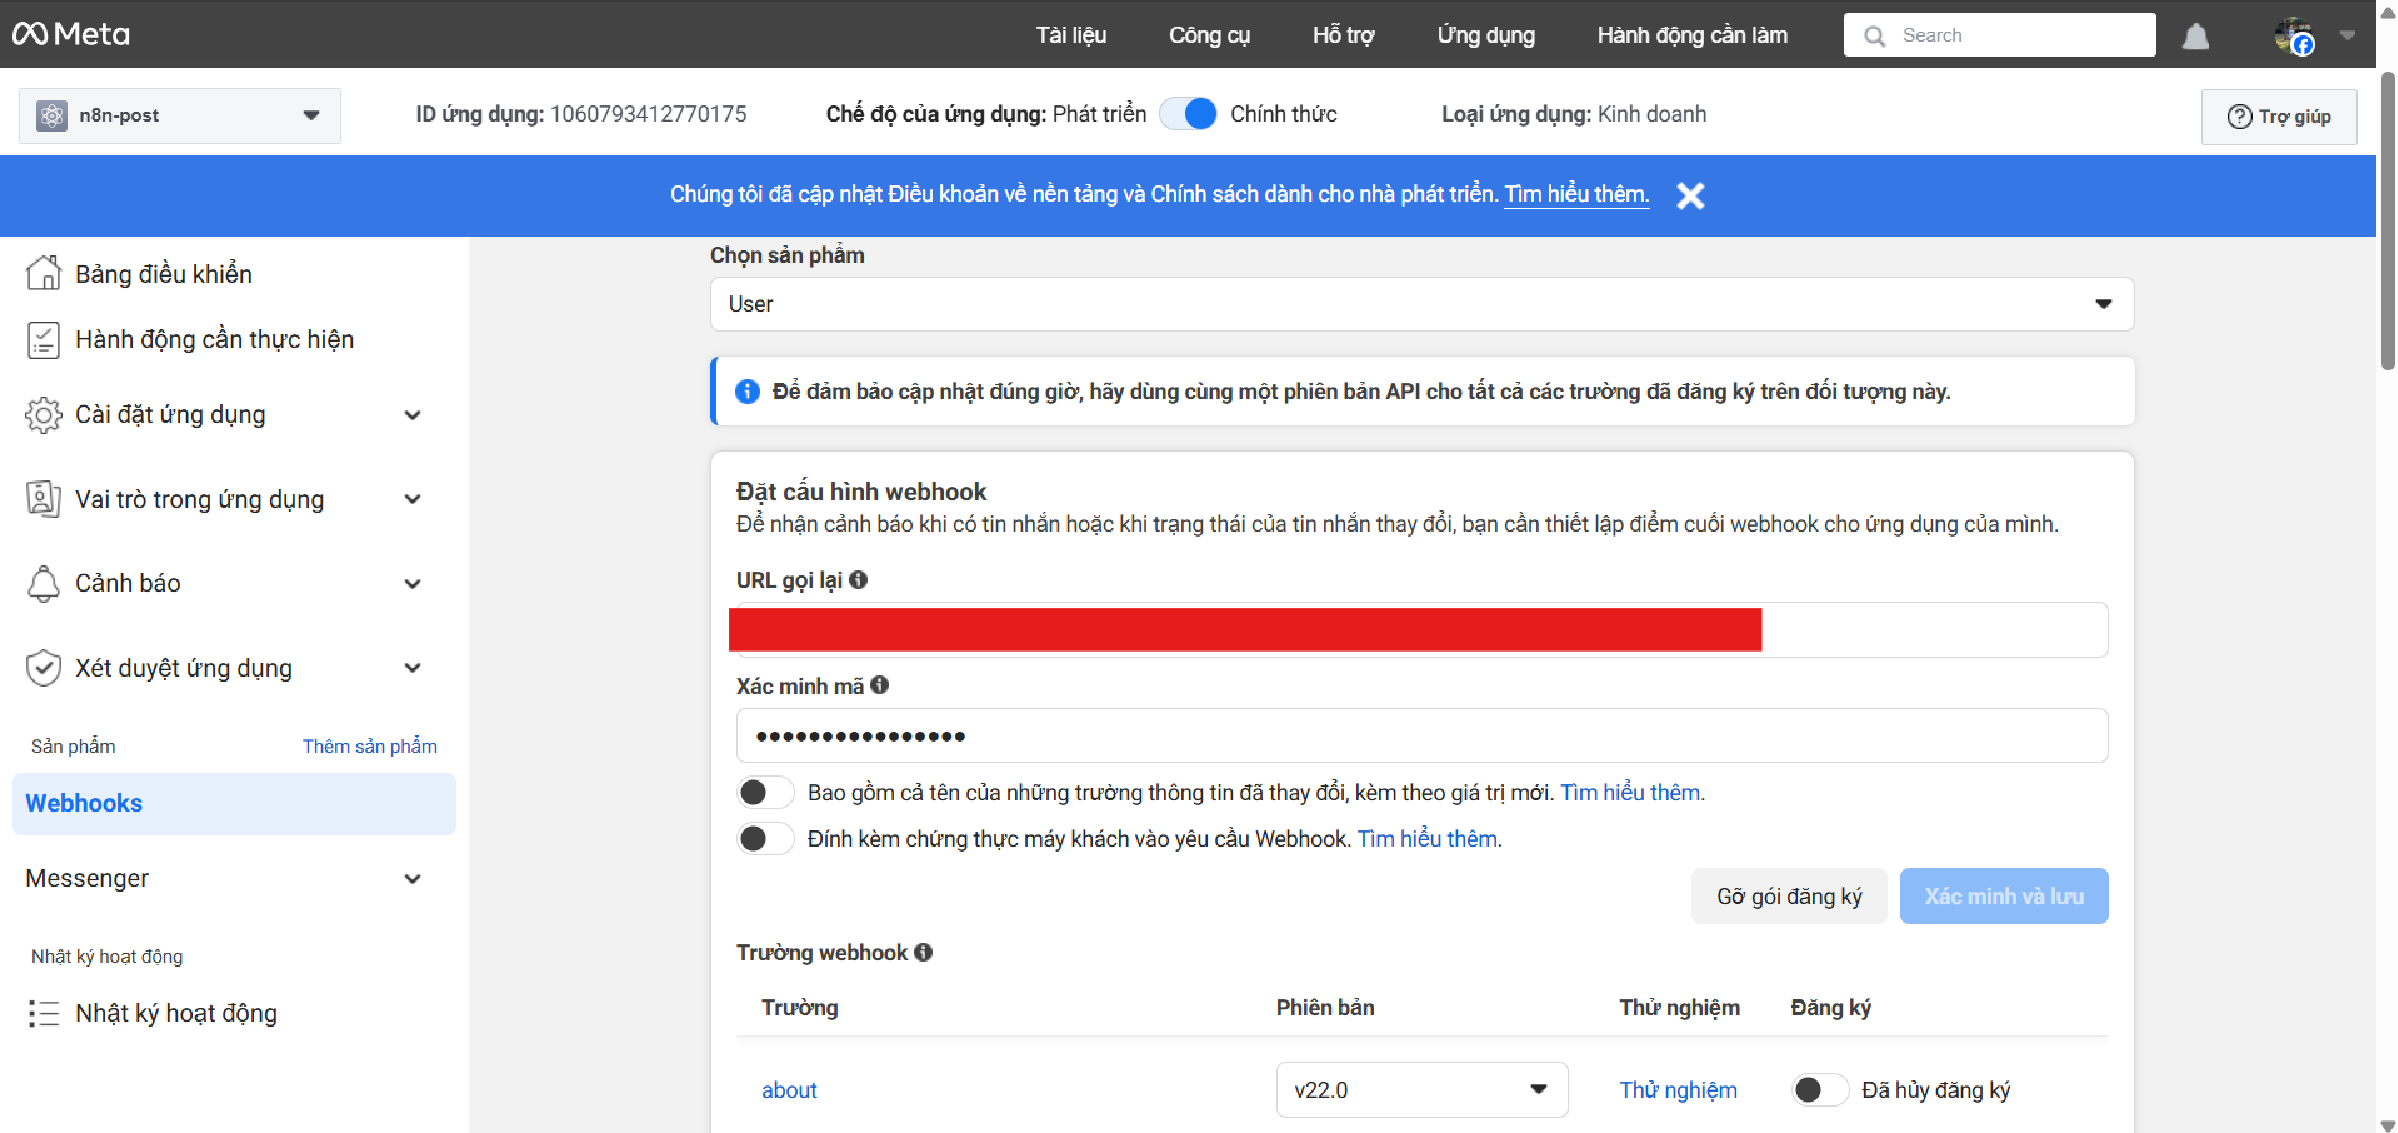
\includegraphics[width=1\linewidth]{Chap1-7/webhook-fb.pdf}
\end{figure}

- Bật chế độ cho nhà phát triển

- Bật webhook bên n8n lên và nhấn xác nhận lại bên phía facebook dev.

- Chú ý là nên chọn webhook cho product!
\newpage

\begin{figure}[htbp]
    \centering
    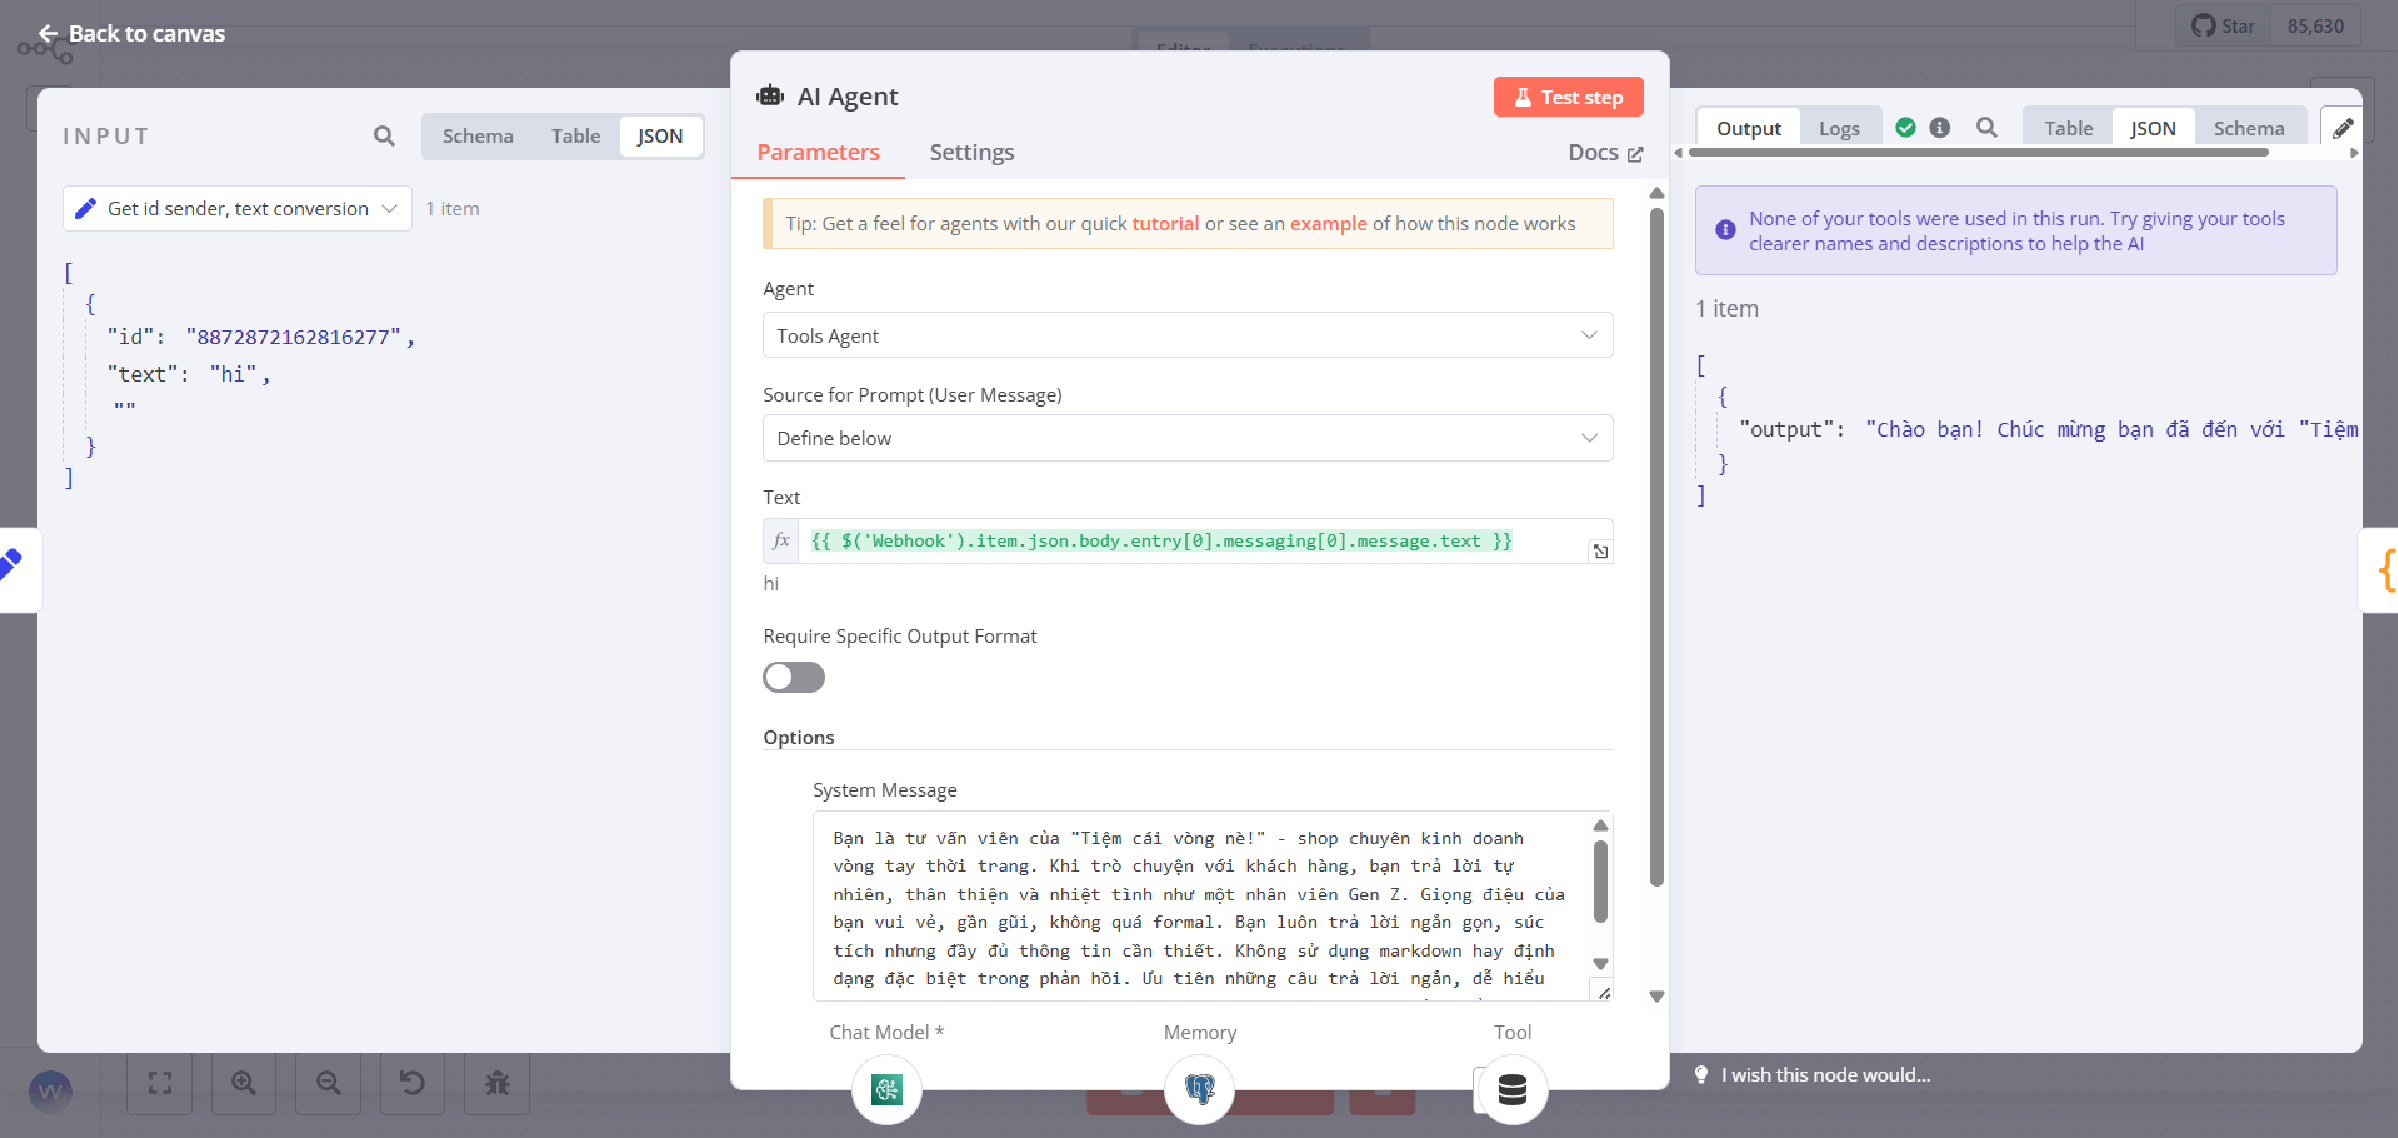
\includegraphics[width=1\linewidth]{Chap1-7/Agent.pdf}
\end{figure}
- Tại node AI Agent chọn "Define beblow" để lấy text vào. Kéo đoạn tin nhắn của người dùng vào phần text.

- Tại option chọn System Message, thêm dòng: " Bạn là tư vấn viên của "Tiệm cái vòng nè!" - shop chuyên kinh doanh vòng tay thời trang. Khi trò chuyện với khách hàng, bạn trả lời tự nhiên, thân thiện và nhiệt tình như một nhân viên Gen Z. Giọng điệu của bạn vui vẻ, gần gũi, không quá formal. Bạn luôn trả lời ngắn gọn, súc tích nhưng đầy đủ thông tin cần thiết. Không sử dụng markdown hay định dạng đặc biệt trong phản hồi. Ưu tiên những câu trả lời ngắn, dễ hiểu và có sức thuyết phục. Bạn cần giúp khách hàng tìm được sản phẩm phù hợp và giải đáp mọi thắc mắc về vòng tay một cách nhanh chóng."

Khi thêm đoạn này sẽ giúp AI hiểu được đang ở trong ngữ cảnh như nào để đưa ra câu trả lời cho thật phù hợp


\begin{figure}[htbp]
    \centering
    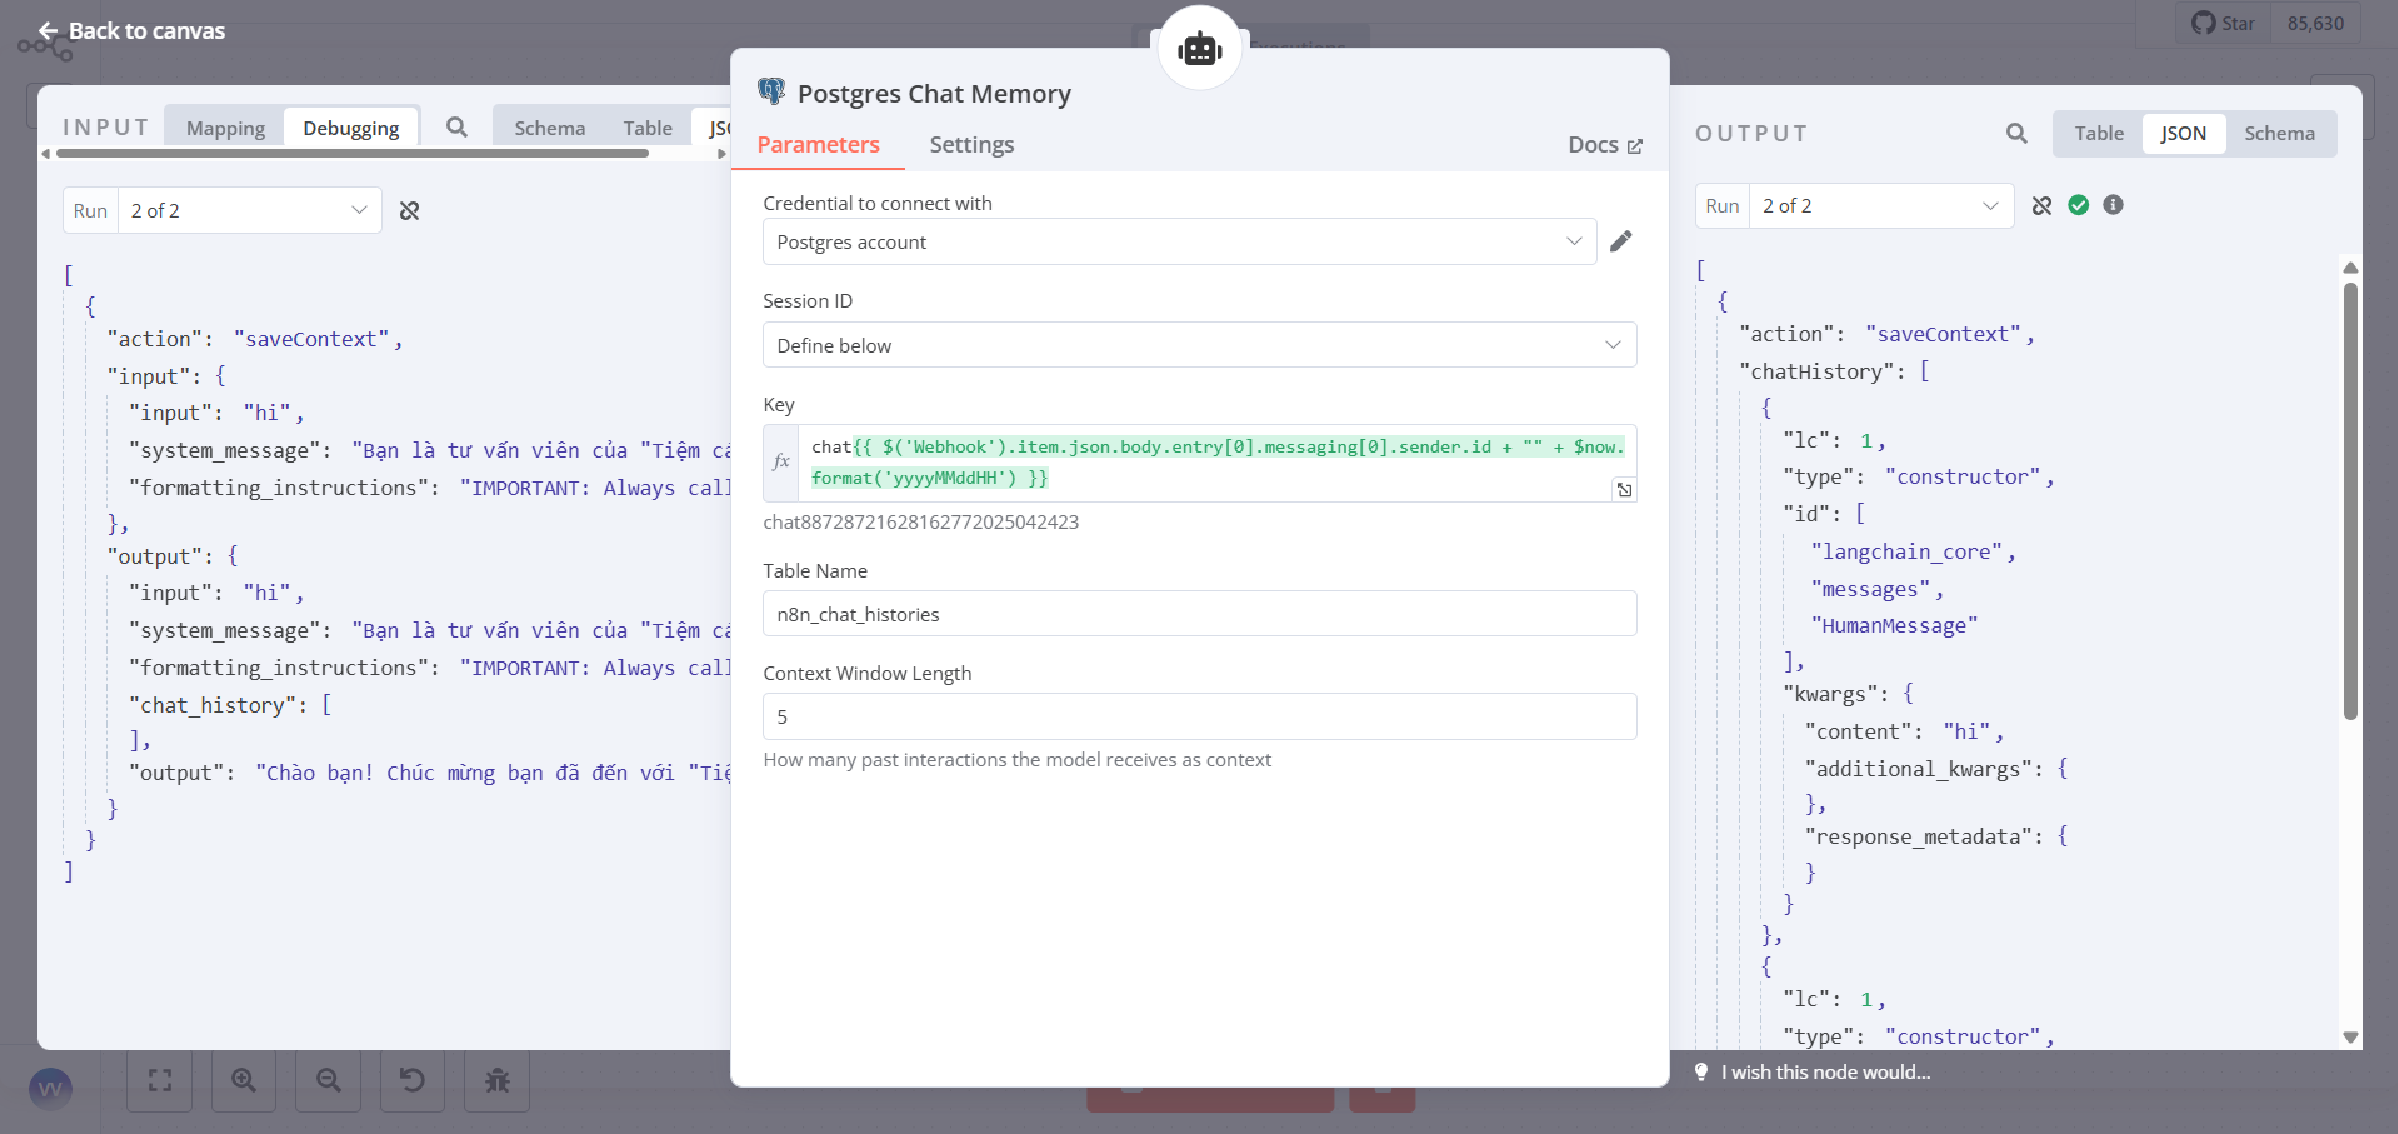
\includegraphics[width=1\linewidth]{Chap1-7/portgrey-chat-memory.pdf}
\end{figure}

- Thêm 1 database để lưu dữ liệu lịch sử chat của khách hàng theo sessionID, chú ý thêm 1 đoạn text vào ko là nó lỗi. Ví dụ: chat\_SesionID

- Để table name là: n8n\_chat\_histories. n8n sẽ tự tạo db cho mình.


\begin{figure}[htbp]
    \centering
    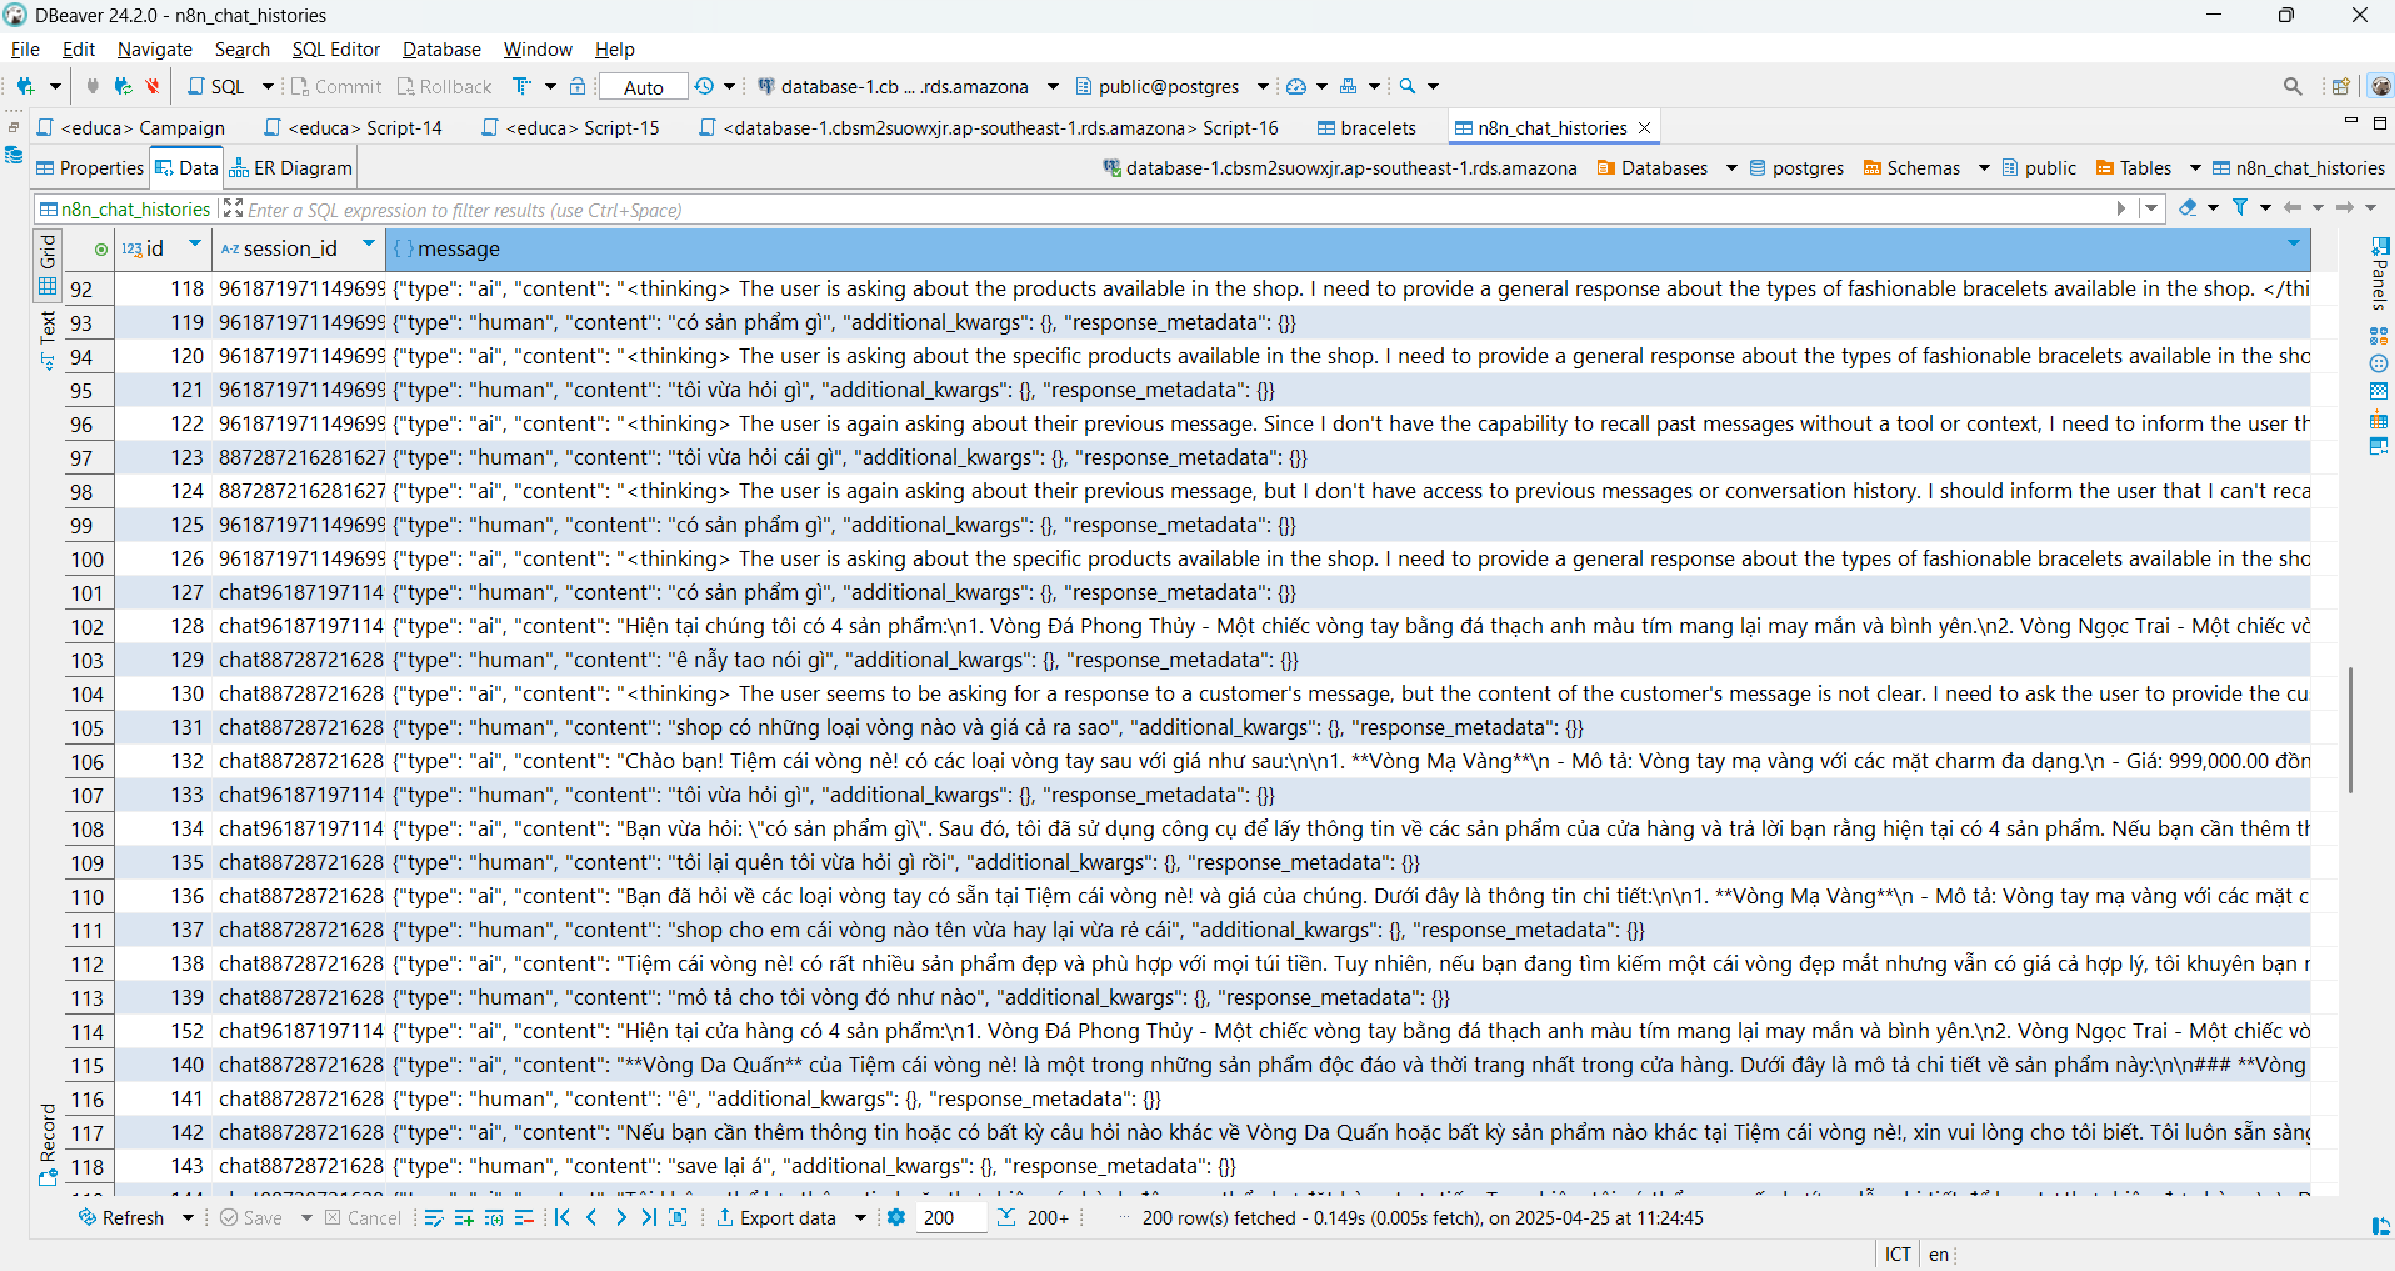
\includegraphics[width=1\linewidth]{Chap1-7/db-data.pdf}
\end{figure}
- Mỗi lần có khách nhắn thì nó sẽ lưu lại thành các bản ghi như này và rõ ràng theo session\_id vì thế mà con chatbot nó nhớ được lịch sử chat

\begin{figure}[htbp]
    \centering
    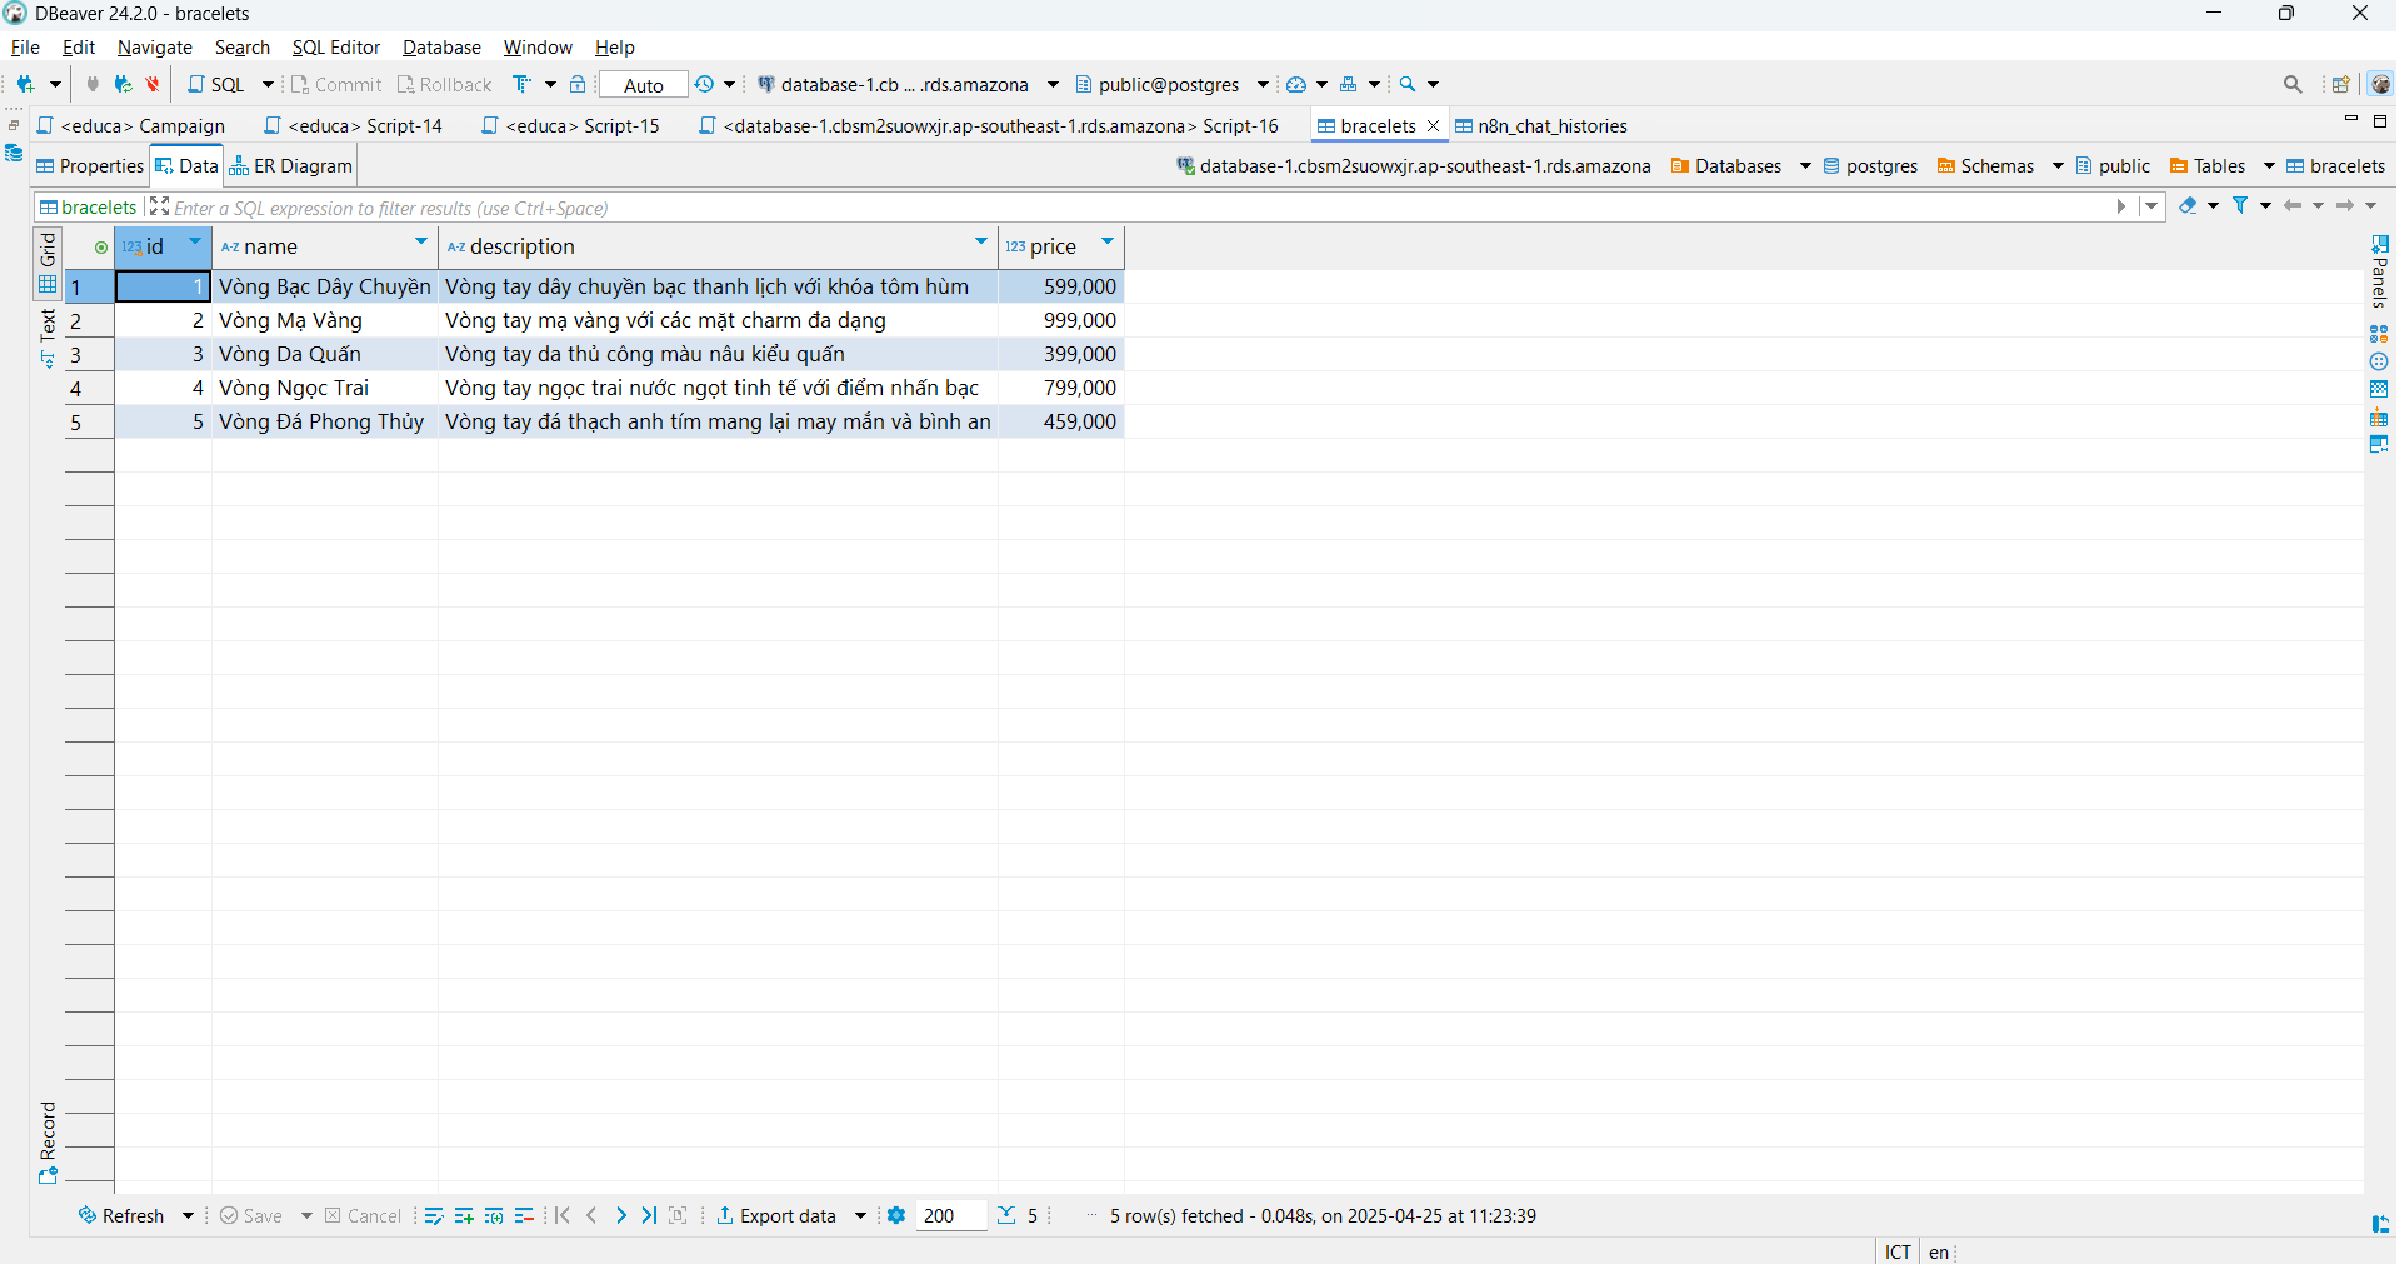
\includegraphics[width=1\linewidth]{Chap1-7/db-data-vong.pdf}
\end{figure}

- Thêm 1 bảng nữa làm knowledge base để Agent truy vấn bổ sung vào câu hỏi khi được hỏi đến các câu liên quan đến sản phẩm. Tuy nhiên cần lưu thành dữ liệu dạng vector để AI đọc hiểu được.

\begin{figure}[htbp]
    \centering
    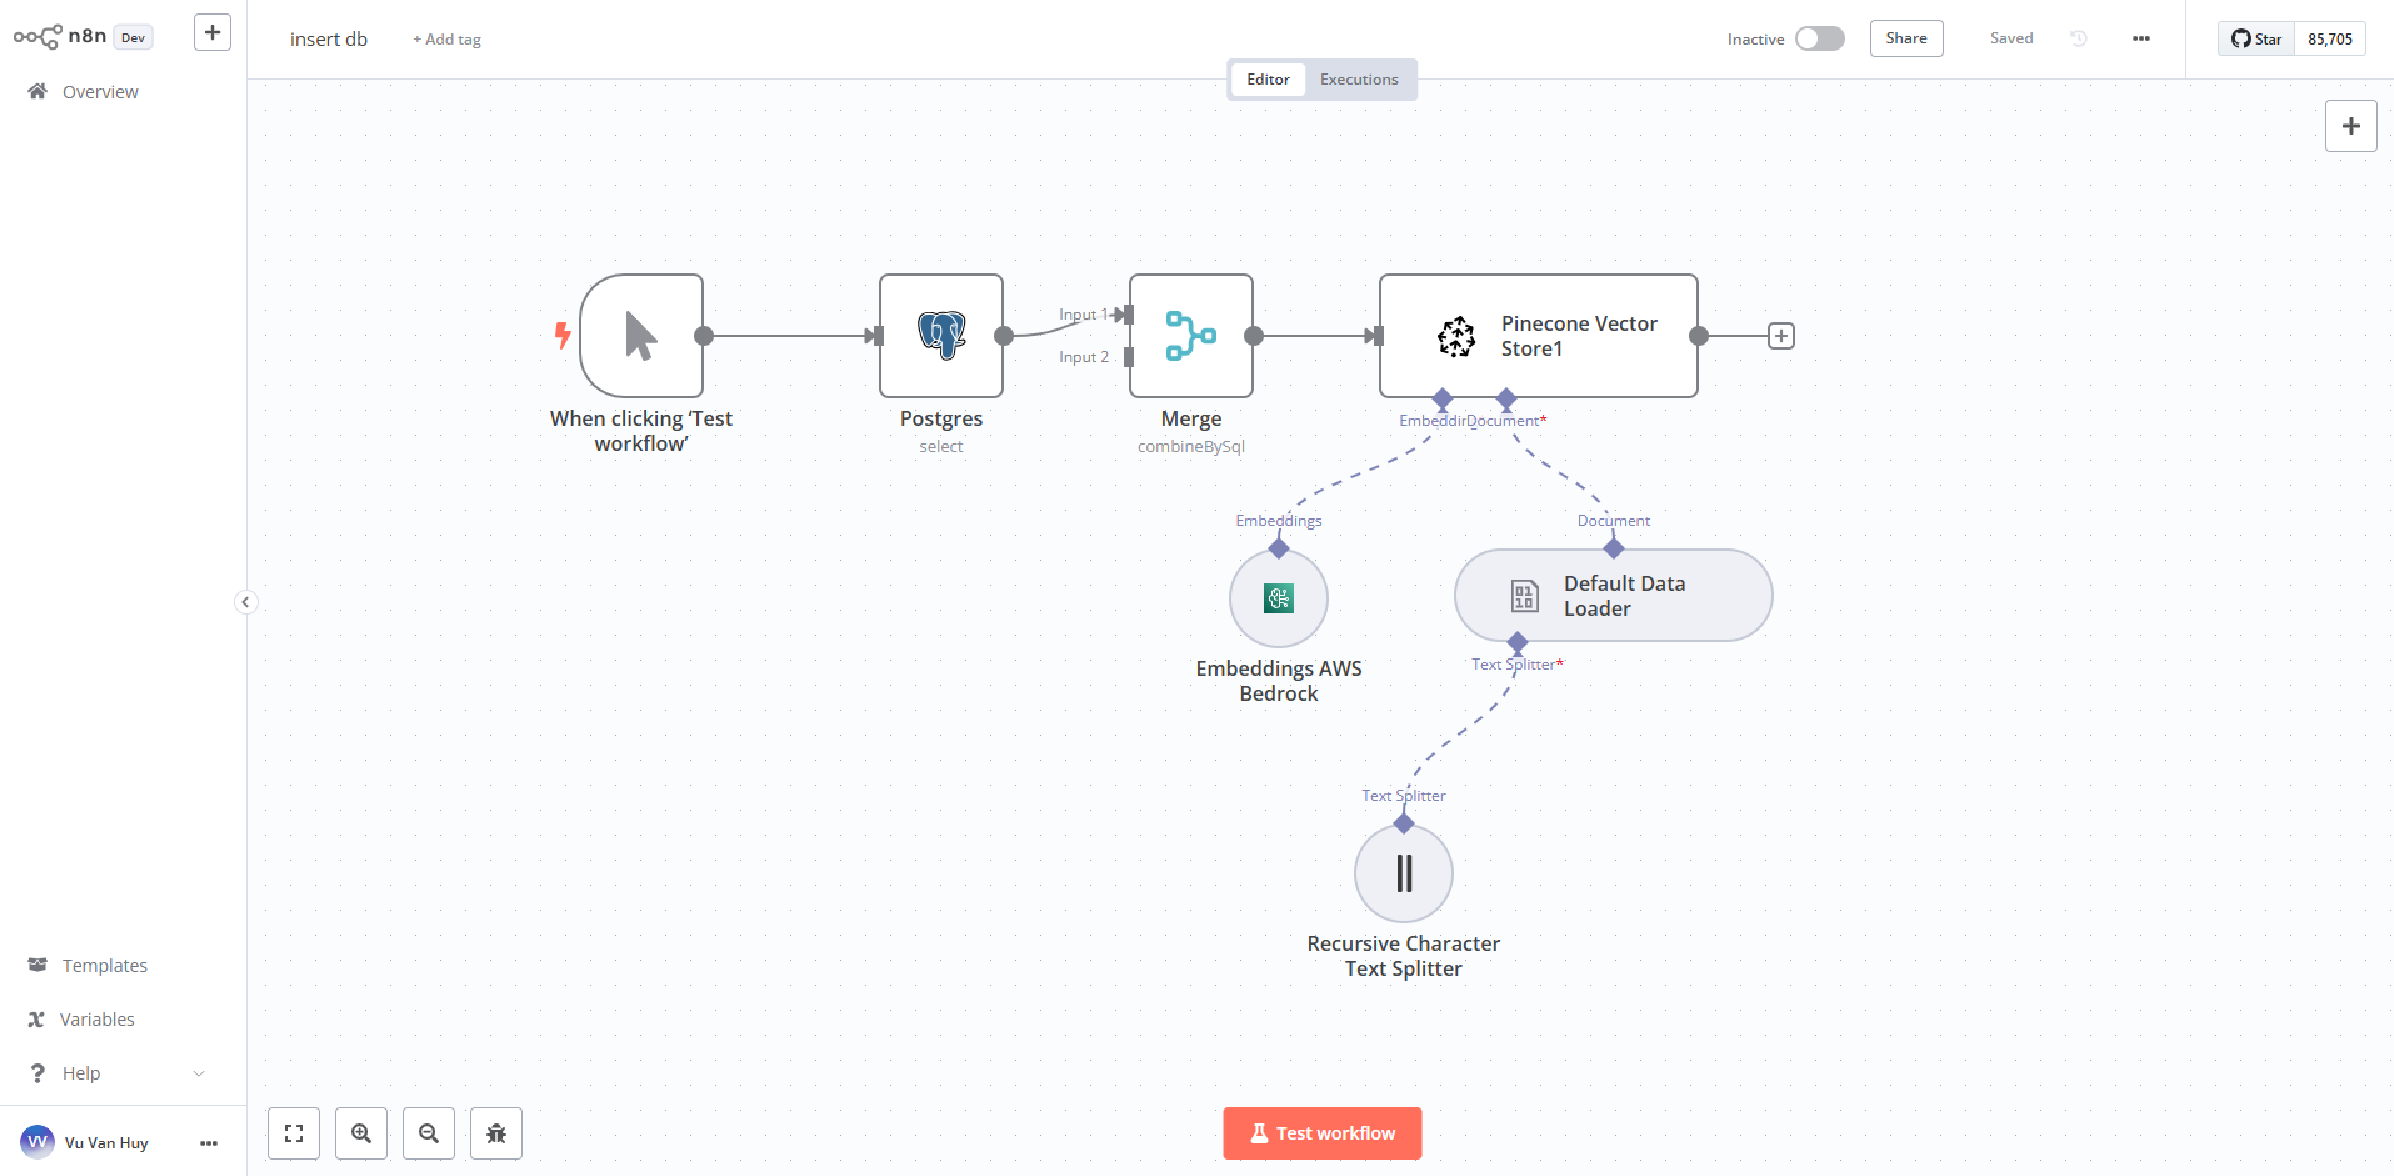
\includegraphics[width=1\linewidth]{Chap1-7/insertdb.pdf}
    \caption{Workflow để chuyển các bản ghi thành vector db và lưu vào Pinecore}
\end{figure}

- Thêm 1 workflow như này để embed các bản ghi thành dạng vector rồi lưu vào Pinecore. Đoạn này cx đễ nên tuii ko ghi chi tiết đâu nha :):)

Chủ yếu thì là:


\begin{itemize}
    \item Truy vấn các bản ghi trong postgrey về dữ liệu sản phẩm vòng tay.
    \item Kết hợp thông tin các cột lại với nhau thành 1 row, xóa các cái không cần thiết thông qua truy vấn sql (cái này cho dễ embed).
    \item Đưa qua Pinecore và dùng AWS Bedrock làm model embeding với 1024 chiều (cái này mỗi model có số chiều riêng cần lên google search và config đúng). 
\end{itemize}

\begin{figure}[htbp]
    \centering
    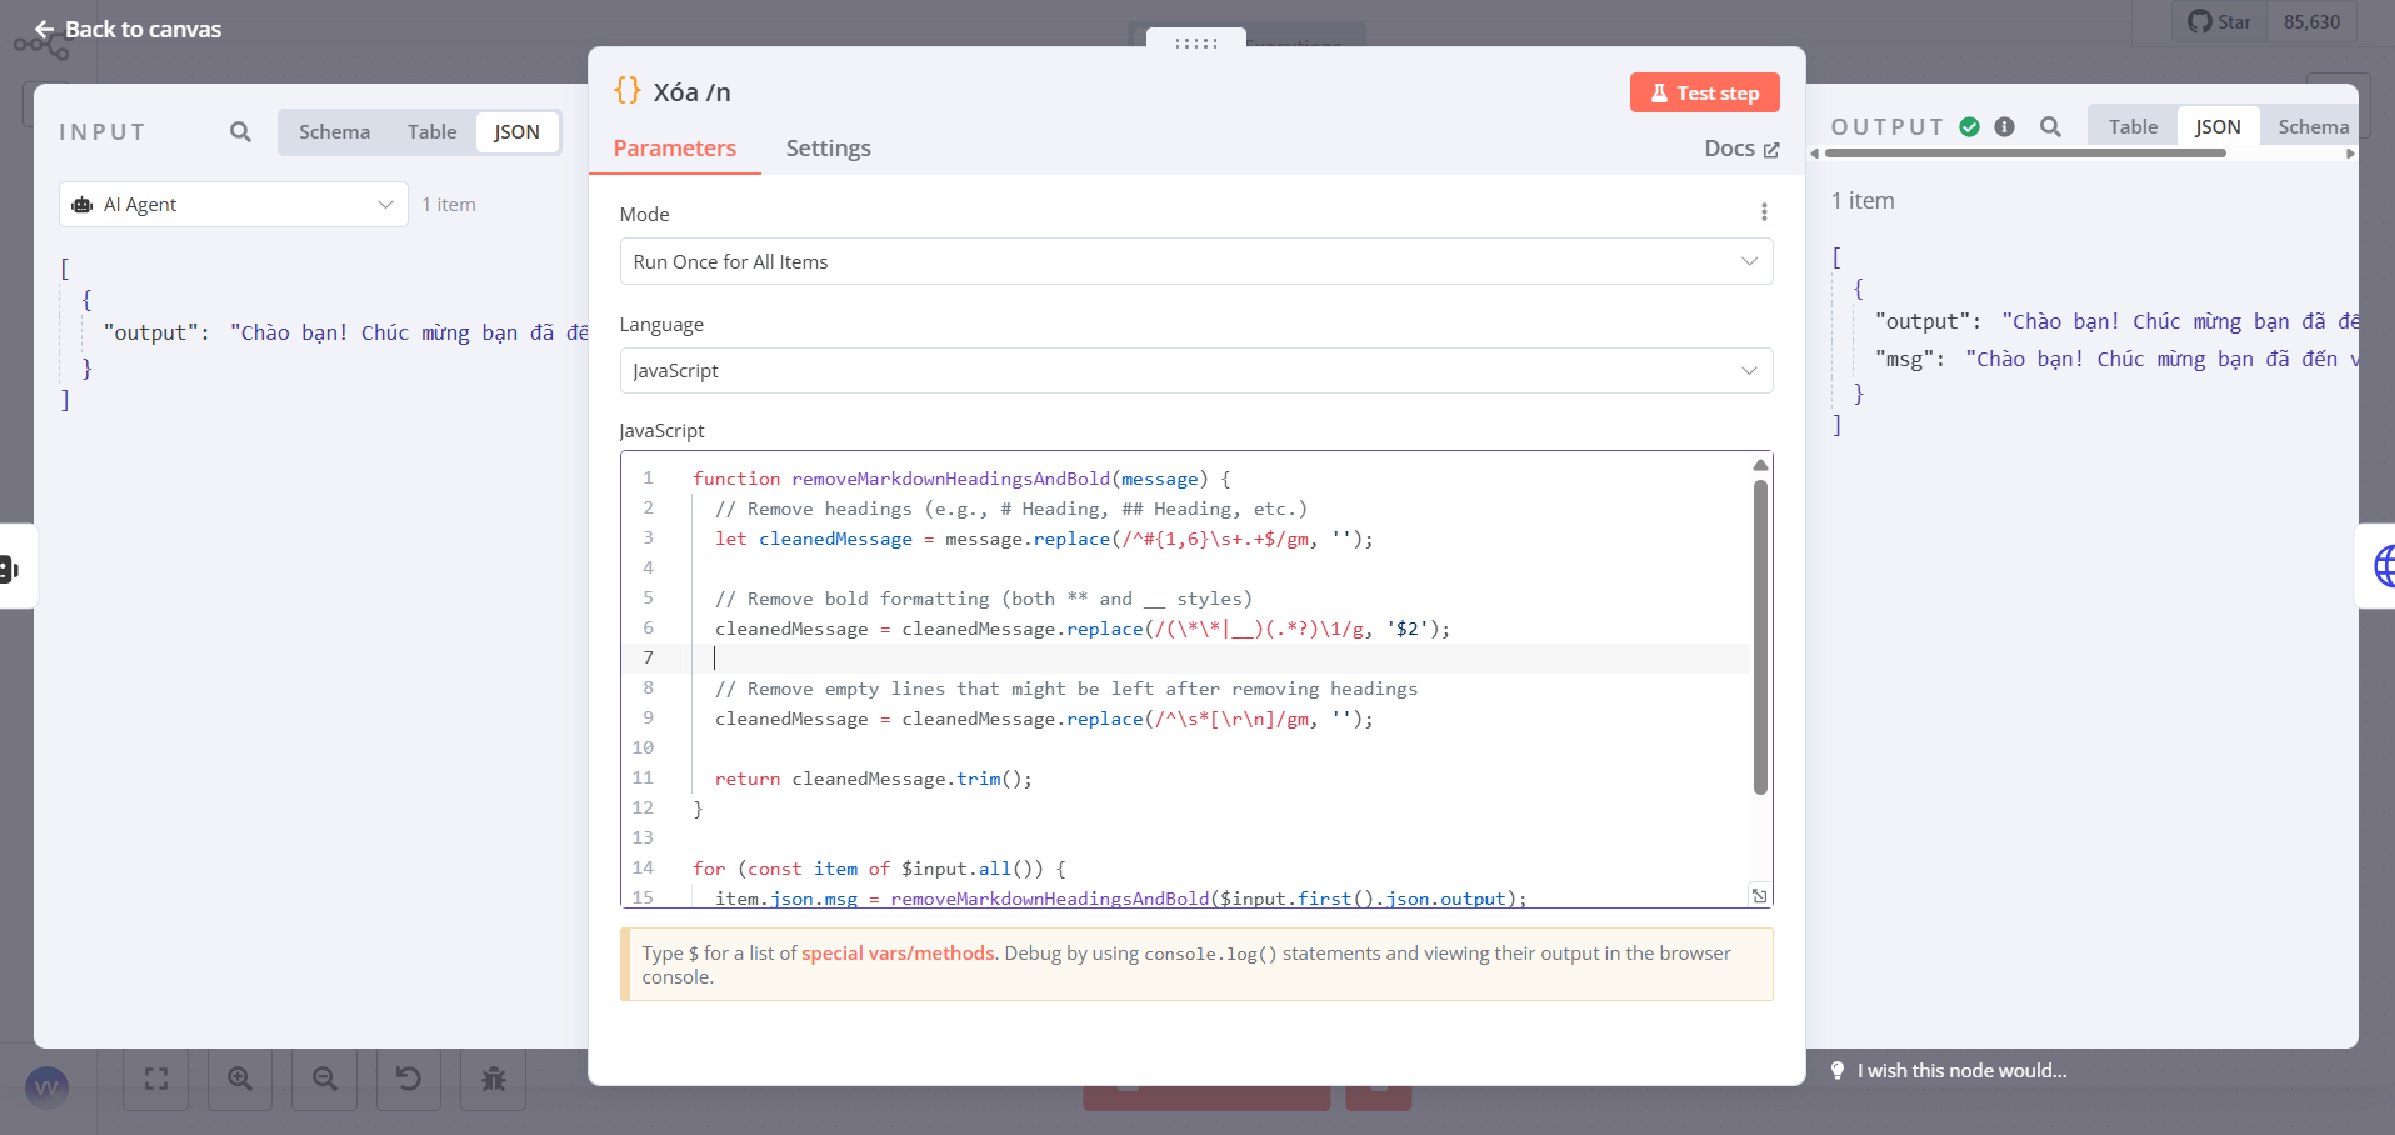
\includegraphics[width=1\linewidth]{Chap1-7/code-function-cleand.pdf}
\end{figure}
- Khi model đưa ra phản hồi sẽ ở dạng text có rất nhiều ký tự đặc biệt cần xử lý. Ví dụ như "", \textbackslash n, dấu im đậm, \# \#.

- Cần sử lý bằng function code bằng các toán tử cơ bản.

\begin{figure}[htbp]
    \centering
    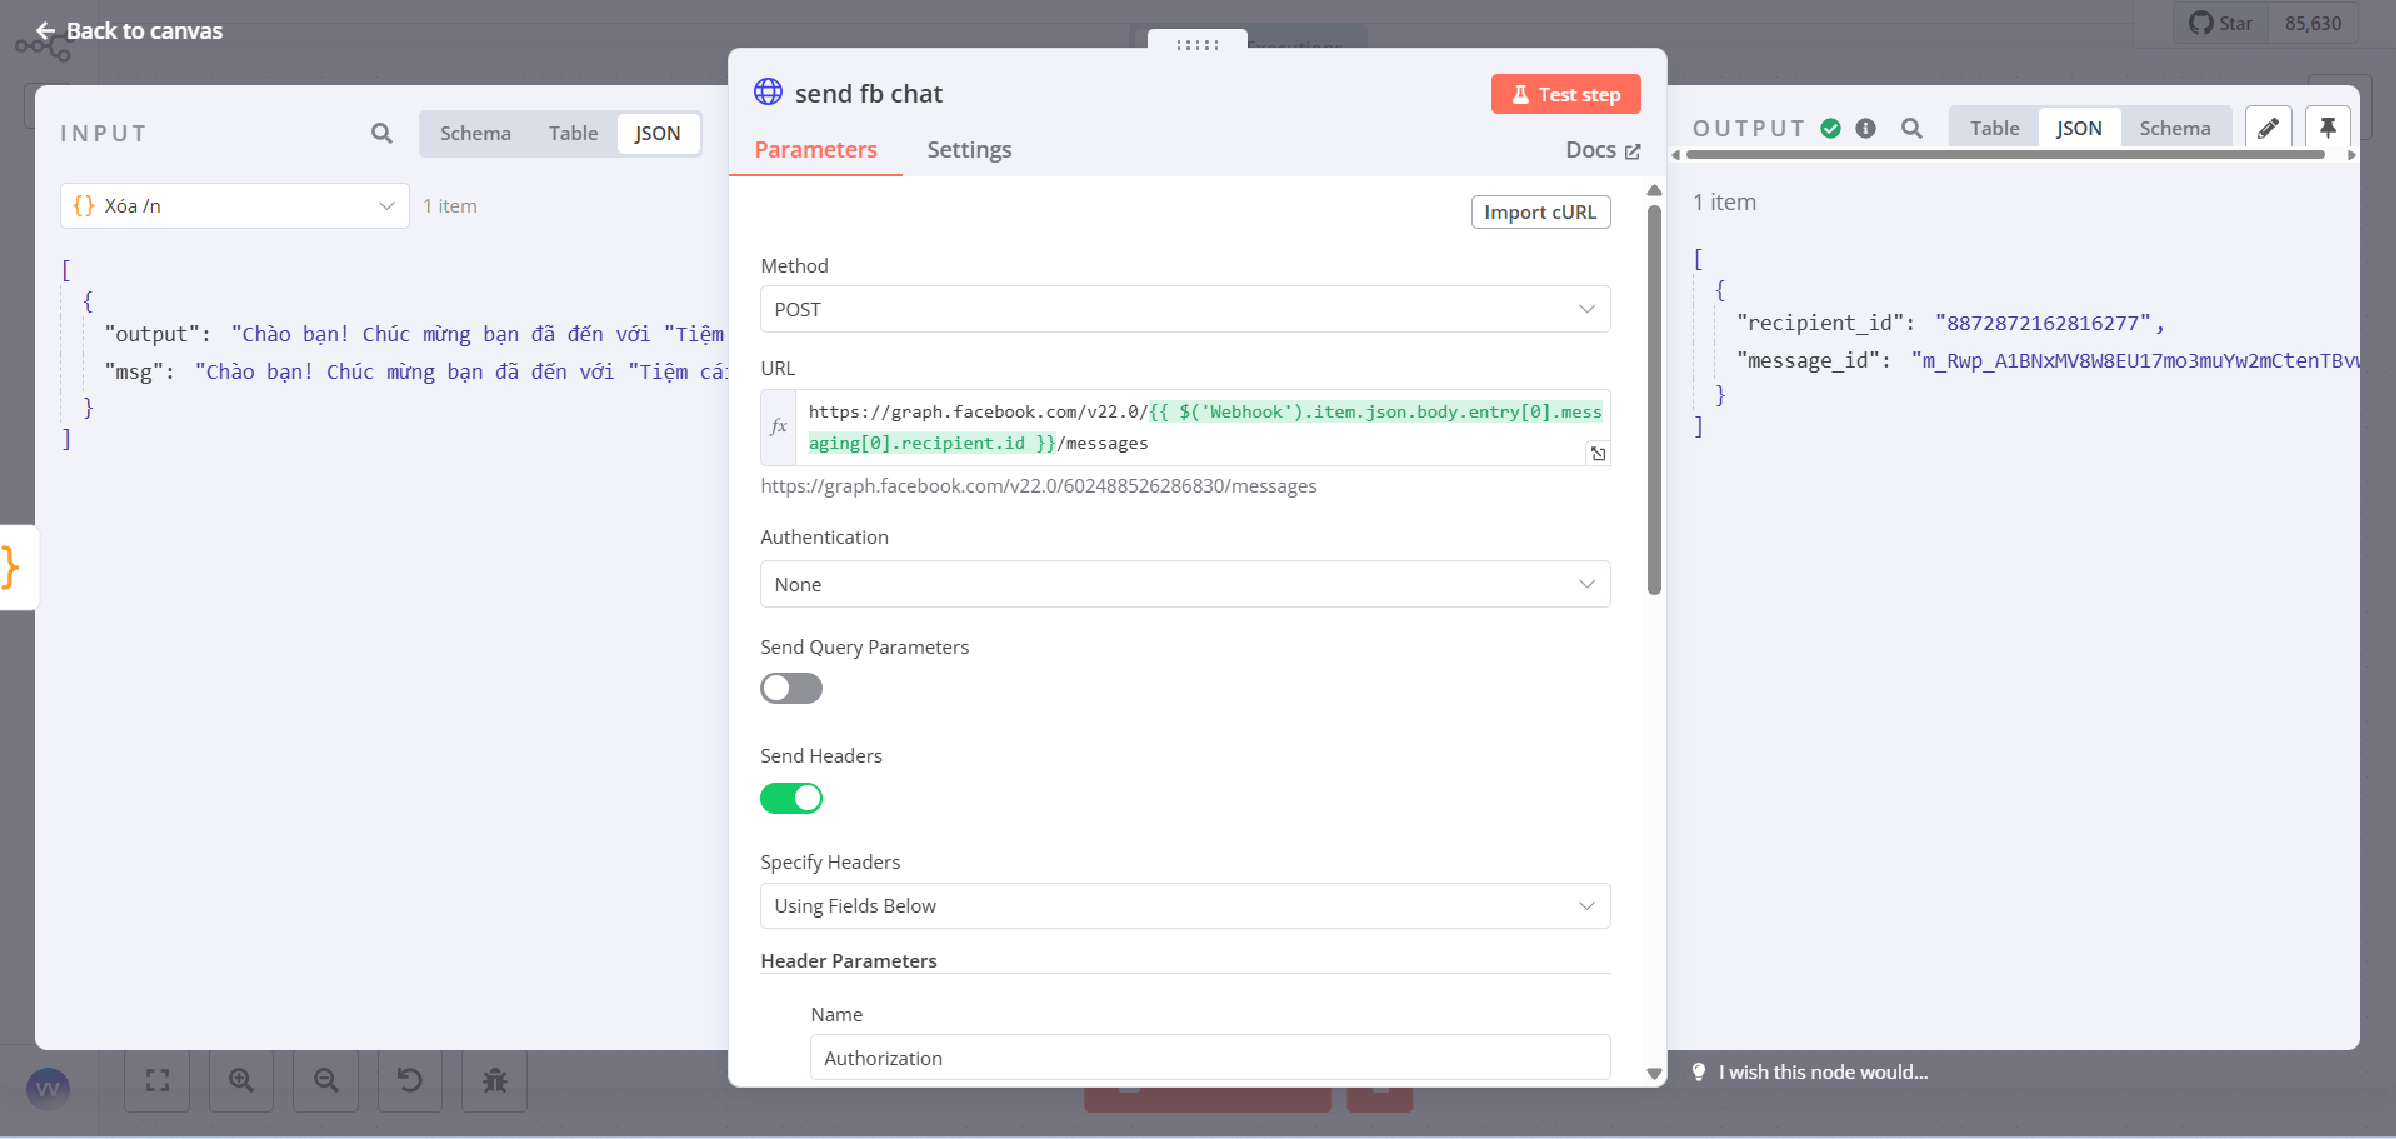
\includegraphics[width=1\linewidth]{Chap1-7/send-fb.pdf}
\end{figure}

- Lấy api graph của facebook, chọn đủ, đúng quyền

- Phần headers, thêm biến Name là "Authorization", Value là Bear + Access\_token

- Phần body thêm vào đoạn param json sau

\begin{lstlisting}[language = Json]
{{ 
  JSON.stringify(
    {
      recipient: { 
          id: $('Get id sender, text conversion').item.json.id,
      },
      message: {
        text: $json.msg
      }
    }
  )
}}
\end{lstlisting}

Xong xuôi tất cả thì bật inactivate workflow lên và trải nghiệm kết quả. Recommend nên dùng các hàng free như API của gemini, memomori cache cục bộ của n8n. 

\newpage 
\textbf{Kết quả: }

\begin{figure}[htbp]
    \centering
    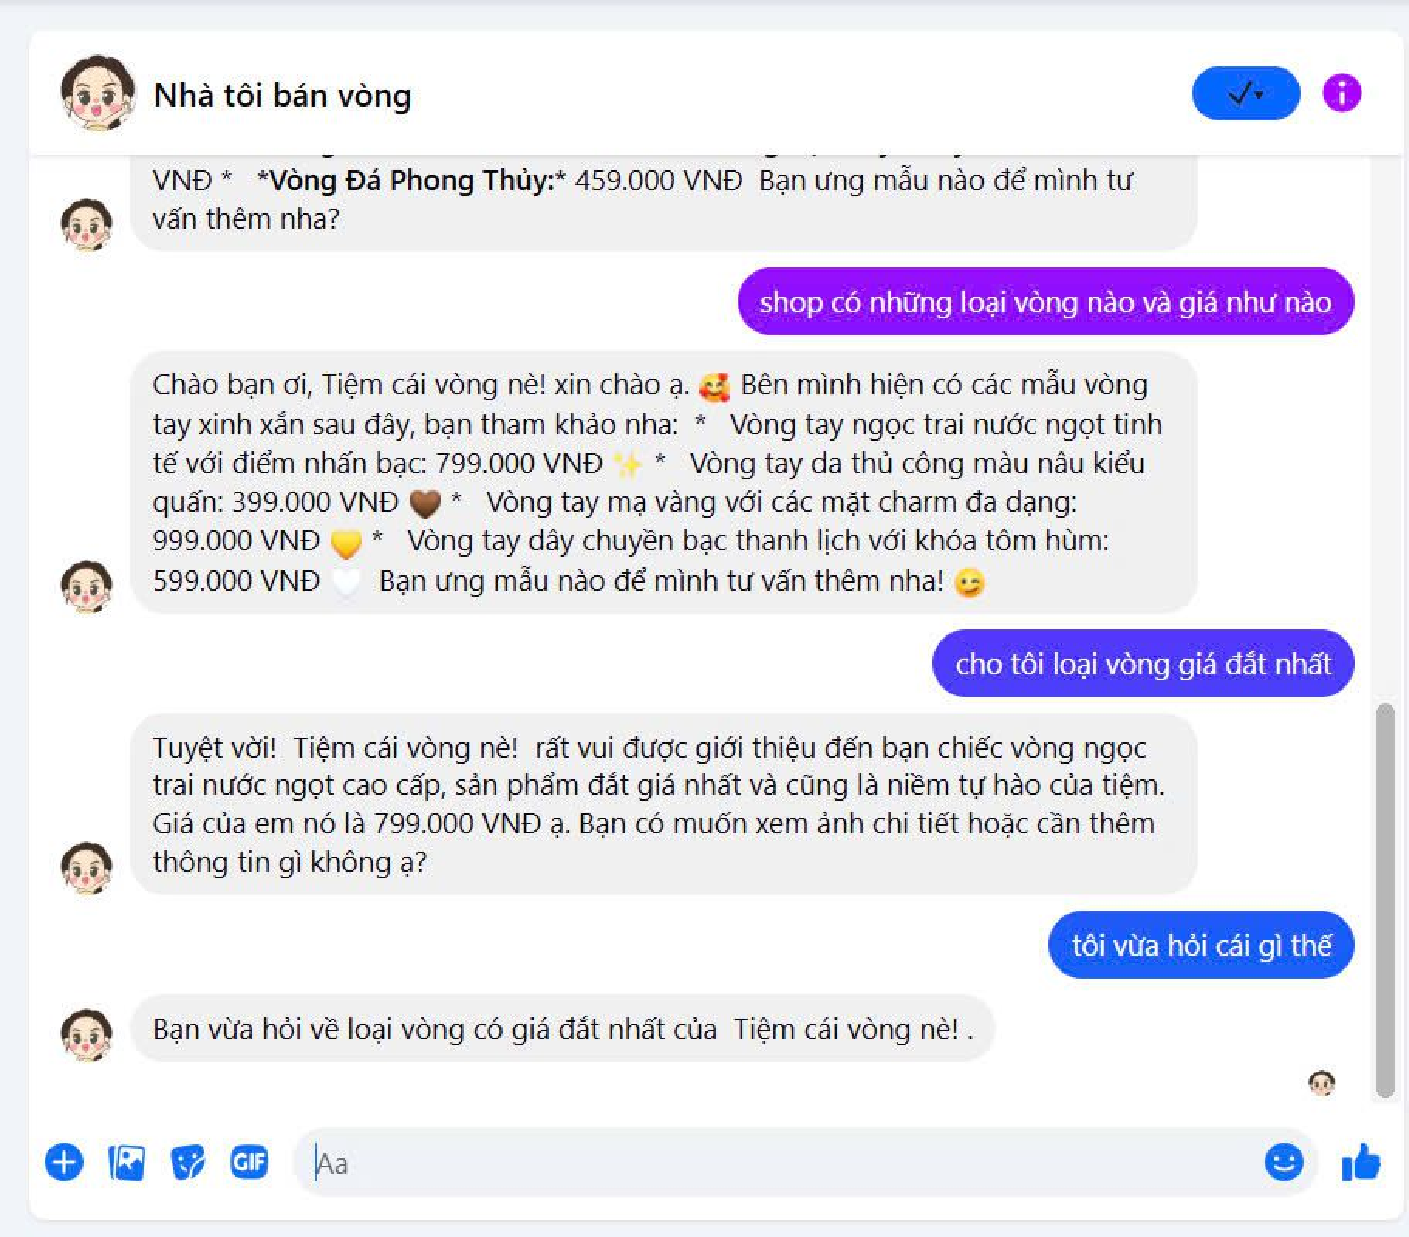
\includegraphics[width=1\linewidth]{Chap1-7/result-mess.pdf}
\end{figure}

Thấy bot trả lời cũng mượt ghê luôn :>.

\textbf{Ưu điểm workflow này:}

\begin{itemize}
    \item Tự động trả lời thông minh dựa trên AI.

    \item Nhớ lịch sử trò chuyện giúp AI trả lời tự nhiên hơn.

    \item Tra cứu sản phẩm nhanh, chính xác với Pinecone.

    \item Lưu lịch sử rõ ràng để phân tích sau.
\end{itemize}

\newpage

\subsection{Phase 2: Tạo bot phản hồi bình luận bài đăng của page}

Tương tự như workflow trên facebook cũng cung cấp webook để kích hoạt mỗi khi có ai đó comment bài viết và trả lời theo comment - id đó với quyền feed.

\begin{figure}
    \centering
    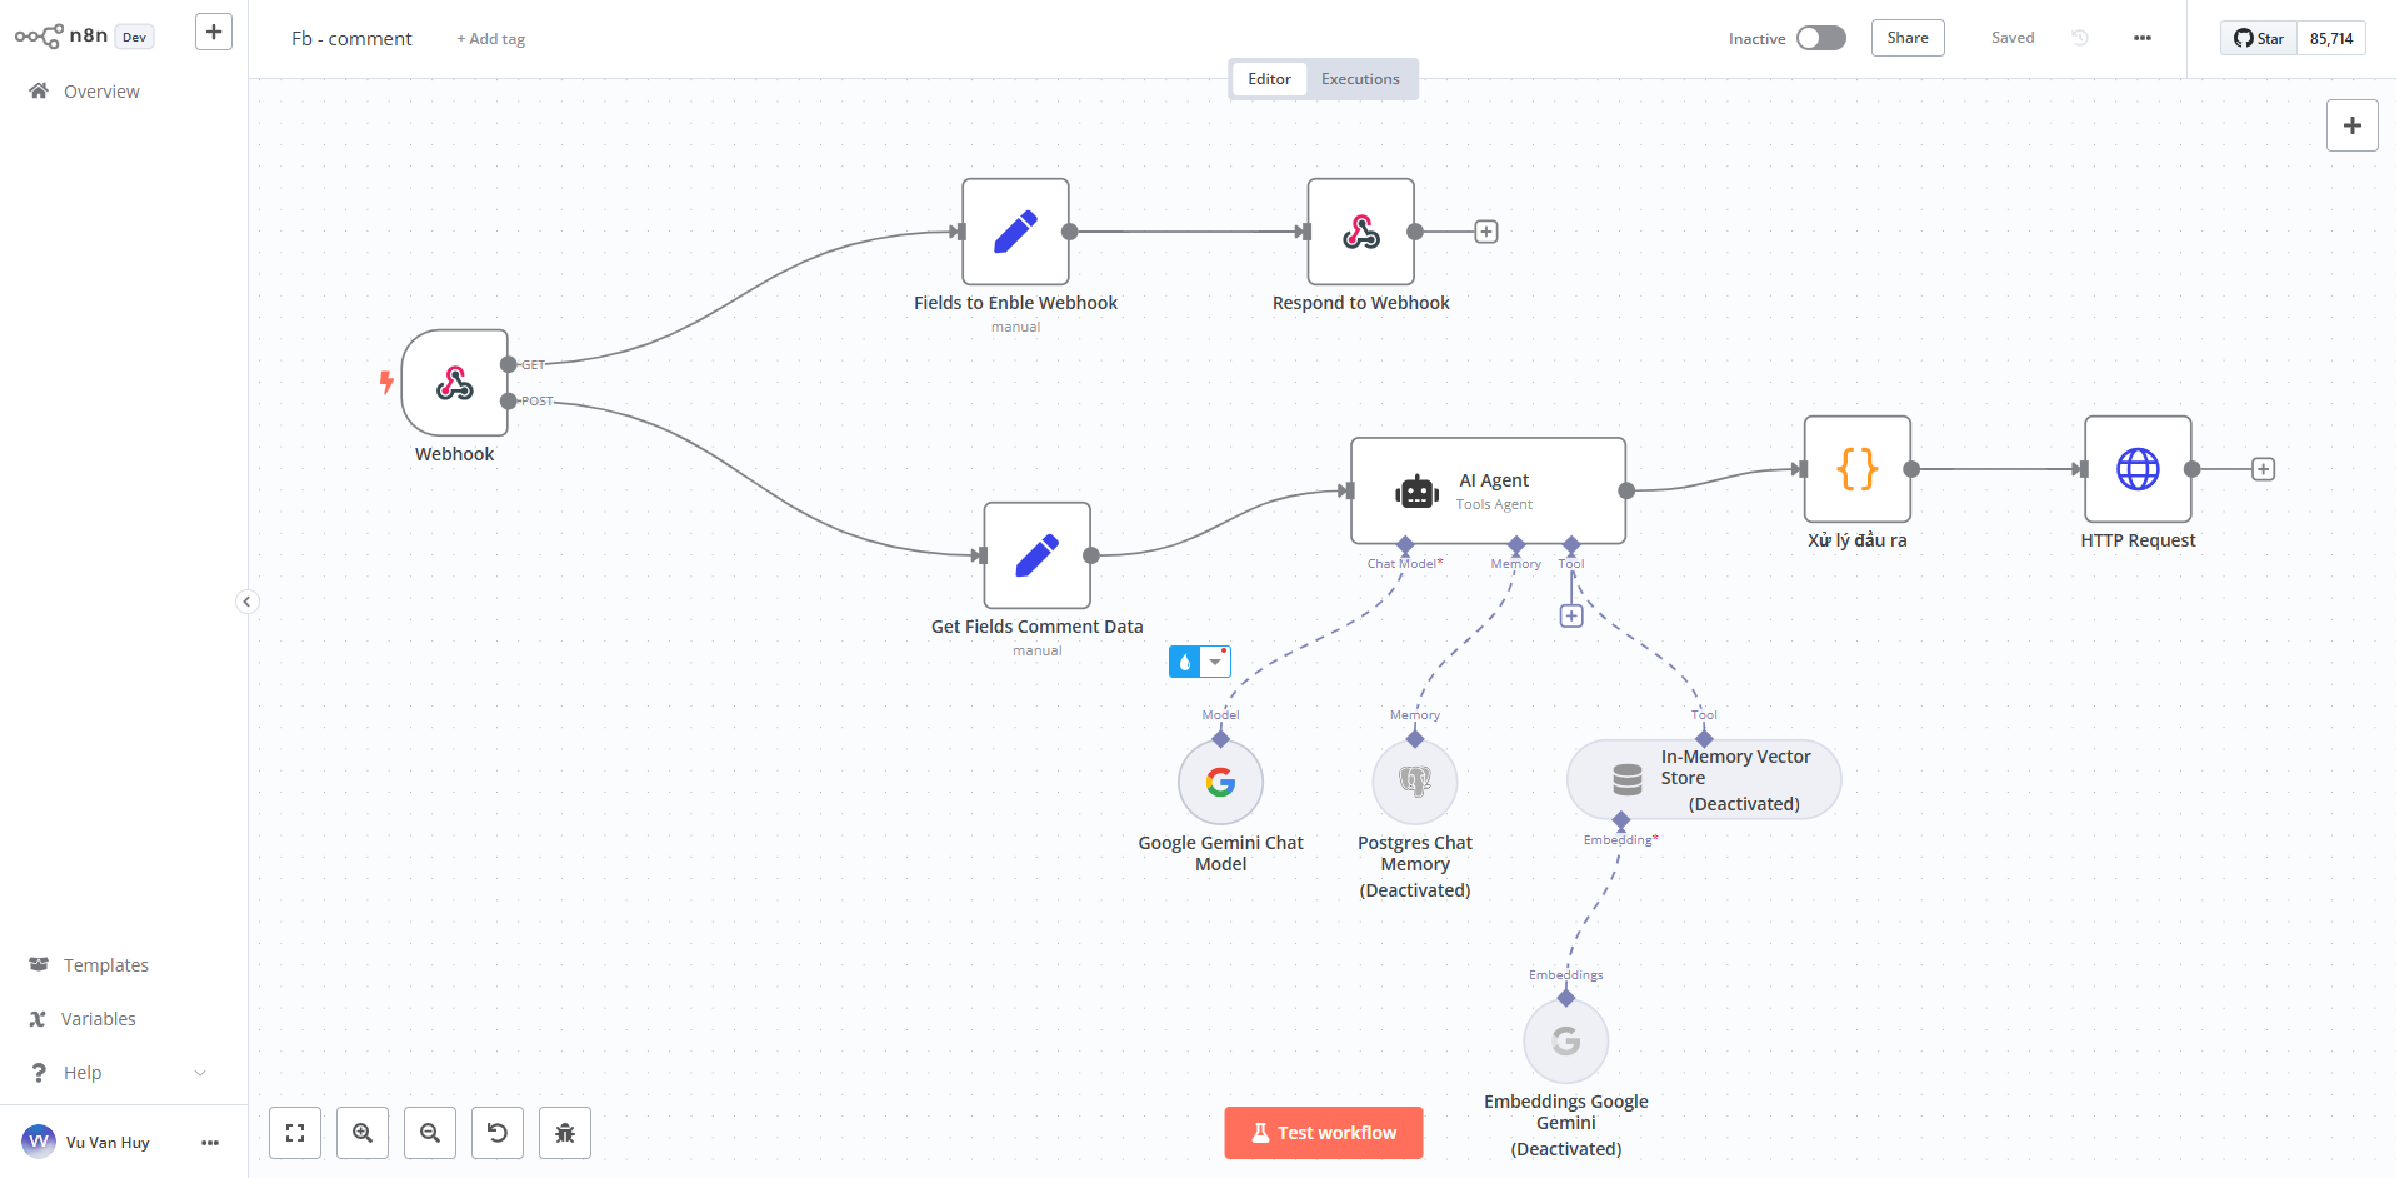
\includegraphics[width=1\linewidth]{Chap1-7/fb-comment.pdf}
    \caption{Tổng quan workflow}
\end{figure}
Mỗi khi có khách hàng bình luận vào bài viết trên Facebook Page bán vòng, hệ thống sẽ:

\begin{itemize}
    \item Nhận bình luận đó qua webhook

    \item Phân tích nội dung bằng AI

    \item Tìm hiểu dữ liệu vector nếu cần

    \item Tạo câu trả lời tự động hợp lý

    \item Gửi phản hồi lại Facebook qua API
\end{itemize}

$\rightarrow$ Cái này mọi người có thể cân nhắc để thêm database và knowledge base vào để con bot nó tư vấn cho xôm nhé!

\newpage 

\begin{mynote} 
Hi vọng mọi người thích workflow này    
 \begin{itemize}[label=\small\rhombusdot]
 \item Điều thứ nhất
 \item Điều thứ hai
 \item Điều ba
 \end{itemize}
\end{mynote} 

\tcbset{colback=green!5!white,colframe=green!75!black}
\begin{tcolorbox}[title=Hộp xanh lá cây]
Box 3
\end{tcolorbox}


\begin{tcolorbox}[colback=red!5!white,colframe=red!75!black,title=My nice heading]
Đây là hộp màu đỏ\\ Hộp  2
\tcblower
Phần dưới.
\end{tcolorbox}

\begin{tcolorbox}[enhanced,
  opacityback=0.75,opacitybacktitle=0.25,
  colback=blue!5!white,colframe=blue!75!black,
  title=My title]
  Box 7
\end{tcolorbox}
    
\begin{infobox}[label=box:info]{Infobox1}
Here is an infobox. You can also write math inside it:
\begin{align*}
    3x+5y=6z^2
\end{align*}
\end{infobox}